\section{Resultados}


\subsection{Simulação}

    \begin{frame}

        \centering
        \href{https://github.com/HeckRodSav/TG/blob/main/documentation/pictures/POLY_3/simul_POLY_3_R_50.gif}{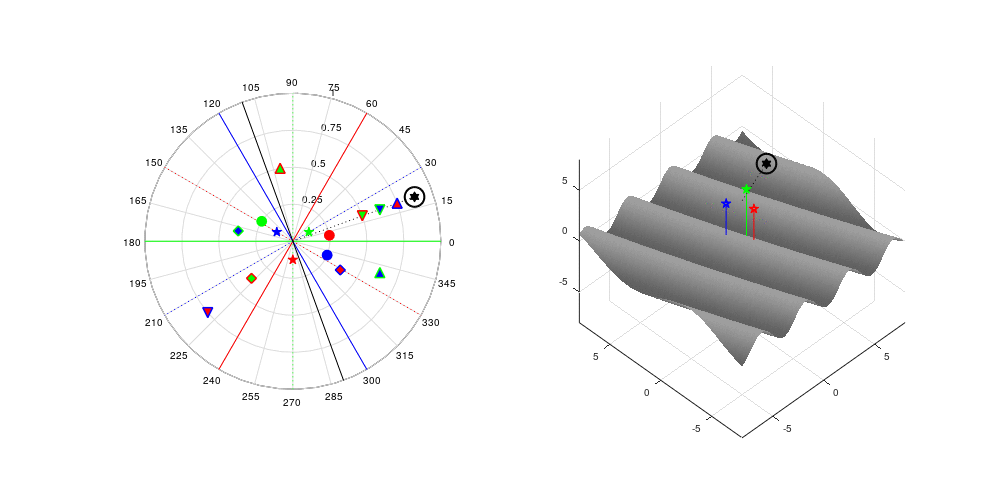
\includegraphics[width=\textwidth]{../pictures/simul_POLY_3_R_50.png}}

    \end{frame}

\subsection{Três antenas}
	\begin{frame}{R\textsuperscript{2} para três antenas}
		\begin{table}
			\centering
			\begin{tabular}{@{}
				S[table-format = 3.1]
				S[table-format = 3.2, table-model-setup = \bfseries]
				S[table-format = 3.2, table-model-setup = \bfseries]
				@{}}
				\toprule
				{SNR (\unit{\deci\bel})} & {R\textsuperscript{2} sem ATT (\unit{\percent})} & {R\textsuperscript{2} com ATT (\unit{\percent})}
				\\\midrule
				\infinity & \bfseries 100.00 & 100.00\\
				20 & 88.06 & 90.45\\
				17 & 88.18 & 87.98\\
				14 & 99.99 & 84.49\\
				7 & 90.12 & 83.50\\
				0 & \bfseries 76.32 & \bfseries 78.73\\
				\bottomrule
			\end{tabular}
			\caption*{\tiny Fonte: Autor, saídas das simulações disponíveis em \href{https://github.com/HeckRodSav/TG/tree/main/documentation/data/POLY_3}{\underline{GitHub}}.}
		\end{table}
	\end{frame}

	\begin{frame}
		\begin{figure}
			\centering
			\caption*{Caso ideal ($\text{SNR} \rightarrow \qty{\infinity}{\deci\bel}$).}
			% \begin{tikzpicture}
    % \pgfsetfillopacity{0.5}

    \def\fileName{simul_POLY_3_R_50}
    \def\fileAddress{../../code/simul/Output/POLY_3/\fileName.dat}
    % \def\fileAddress{../data/\fileName.dat}

    \def\height{.225\linewidth}
    \def\width{0.75\linewidth}
    \def\distance{0.25cm}
    \def\xmin{-1}
    \def\xmax{101}

    \begin{axis} %configuração do eixo Y esquerdo e eixo X
    [
        name=plot1,
        reverse legend, % inverte a ordem que os items aparecem na legenda
    	% legend style={
        % 	at=(current bounding box.north),
        % 	anchor=south,
        % 	legend columns=6,
        % 	transpose legend,
        % 	draw=none,
        % 	/tikz/every even column/.append style={column sep=0.5cm}
    	% }, % onde exibir
        % axis x line=center,
        % axis y line=center,
        height=\height, % altura da região do gráfico
        width=\width, % largura da região do gráfico
        scale only axis, %
        minor grid style={densely dotted}, % estilo da grade secundária
        major grid style={densely dashed}, % estilo da grade principal
        grid style={lightgray, thin}, % cor das grades
        % axis on top, % forçar grade para ficar por cima do gráfico
        %
        %
        % axis y line*=left, % define gráfico para usar eixo esquerdo sem exibir direito
        y tick label style={
            /pgf/number format/.cd,
            fixed,
            % fixed zerofill,
            precision=1, % quantidade de casas depois da virgula
            /tikz/.cd
        },
        % y filter/.expression={y==0 ? NaN : y},
        scaled y ticks = false,
        ylabel={$\alpha_{k}\pm \beta_{k}$ (\si{\radian})}, % titulo eixo vertical
        % yticklabel={\pgfmathparse{\tick-50}\pgfmathprintnumber{\pgfmathresult}}, % fator multiplicativo para valores do eixo
        y tick label style={/pgf/number format/1000 sep=}, % Altera marcação de milhar
        % yticklabel style={rotate=90},
		ytick={-3.1415, -1.5708, 0, 1.5708, 3.1415},
		yticklabels={$-\pi$,$-\dfrac{\pi}{2}$,$0$,$\dfrac{\pi}{2}$,$\pi$},
        % ytick={0,1,2,3,4,5}, % lista de valores a serem utilizados no eixo
        % ymin=-1,  ymax=4,  % intervalo de valores no eixo y -> na dúvida, deixe comentado
        %
        ymajorgrids=true, % exibir grade principal y
        yminorgrids=true, % exibir grade secundária y
        minor y tick num=4, % contagem de linhas na grade secundária y
        % ybar,
        %
        %
        xlabel={$\theta_{DoA}$ (\si{\radian})}, % título eixo horizontal
        % xticklabel={\pgfmathparse{\tick-50}\pgfmathprintnumber{\pgfmathresult}}, % fator multiplicativo para valores do eixo
        % xticklabels={}, % fator multiplicativo para valores do eixo
		% xtick={0, 12.5, 25, 37.5, 50, 62.6, 75, 87.5, 100},
		% xticklabels={$-2~\pi$,$-\dfrac{3~\pi}{2}$,$-\pi$,$-\dfrac{\pi}{2}$,$0$,$-\dfrac{\pi}{2}$,$\pi$,$-\dfrac{3~\pi}{2}$,$2~\pi$},
		xtick={0, 25, 50, 75, 100},
		xticklabels={$-2 \pi$,$-\pi$,$0$,$\pi$,$2 \pi$},
        % xmode=log,
        % log ticks with fixed point,
        % x filter/.code=\pgfmathparse{#1 + 6.90775527898214},
        x tick label style={
            /pgf/number format/.cd,
            fixed,
            % fixed zerofill,
            precision=1,
            /tikz/.cd,
            /pgf/number format/use comma
        },
        xmin=\xmin, xmax=\xmax, % intervalo de valores no eixo x -> na dúvida, deixe comentado
        scaled x ticks = false,
        %
        xmajorgrids=true, % exibir grade principal x
        xminorgrids=true, % exibir grade secundária x
        minor x tick num=7, % contagem de linhas na grade secundária x
        %
        %
        %
        % unbounded coords=jump,
        % jump threshold/.initial=0.25
    ]

	\addplot[
        cmyk_G,
        mark=triangle*,
		opacity=0.5,
        only marks,
        % smooth
    ] table [
        % col sep=comma,
        x=percent, % cabeçalho da coluna de dados X no arquivo
        y=delta_1_x_3, % cabeçalho da coluna de dados Y no arquivo
    ]
    {\fileAddress};	\label{\fileName.1.1}

    \addplot[
        cmyk_G,
        mark=triangle*,
		opacity=0.5,
		mark options={rotate=180},
        only marks,
        % smooth
    ] table [
        % col sep=comma,
        x=percent, % cabeçalho da coluna de dados X no arquivo
        y=delta_3_x_1, % cabeçalho da coluna de dados Y no arquivo
    ]
    {\fileAddress};	\label{\fileName.1.2}

	\addplot[
        cmyk_B,
        mark=triangle*,
		opacity=0.5,
        only marks,
        % smooth
    ] table [
        % col sep=comma,
        x=percent, % cabeçalho da coluna de dados X no arquivo
        y=delta_2_x_1, % cabeçalho da coluna de dados Y no arquivo
    ]
    {\fileAddress};	\label{\fileName.1.3}

    \addplot[
        cmyk_B,
        mark=triangle*,
		opacity=0.5,
		mark options={rotate=180},
        only marks,
        % smooth
    ] table [
        % col sep=comma,
        x=percent, % cabeçalho da coluna de dados X no arquivo
        y=delta_1_x_2, % cabeçalho da coluna de dados Y no arquivo
    ]
    {\fileAddress};	\label{\fileName.1.4}

	\addplot[
        cmyk_R,
        mark=triangle*,
		opacity=0.5,
        only marks,
        % smooth
    ] table [
        % col sep=comma,
        x=percent, % cabeçalho da coluna de dados X no arquivo
        y=delta_3_x_2, % cabeçalho da coluna de dados Y no arquivo
    ]
    {\fileAddress};	\label{\fileName.1.5}

    \addplot[
        cmyk_R,
        mark=triangle*,
		opacity=0.5,
		mark options={rotate=180},
        only marks,
        % smooth
    ] table [
        % col sep=comma,
        x=percent, % cabeçalho da coluna de dados X no arquivo
        y=delta_2_x_3, % cabeçalho da coluna de dados Y no arquivo
    ]
    {\fileAddress};	\label{\fileName.1.6}

    \end{axis}

    % \begin{axis} %configuração do eixo Y direito e legenda
    % [
    %     legend cell align=left, % alinhamento de texto na legenda
    %     % legend pos={outer north east}, % onde exibir caixa de legenda
    %     % reverse legend, % inverte a ordem que os items aparecem na legenda
    % 	legend style={
    %     	at=(current bounding box.north),
    %     	anchor=south,
    %     	legend columns=2,
    %     % 	transpose legend,
    %     	draw=none
    % 	}, % onde exibir
    %     % axis x line=center,
    %     % axis y line=center,
    %     height=\height, % altura da região do gráfico
    %     width=\width, % largura da região do gráfico
    %     scale only axis, %
    %     minor grid style={densely dotted}, % estilo da grade secundária
    %     major grid style={densely dashed}, % estilo da grade principal
    %     grid style={lightgray, thin}, % cor das grades
    %     % axis on top, % forçar grade para ficar por cima do gráfico
    %     %
    %     %
    %     axis y line*=right, % define gráfico para usar eixo direito sem exibir esquerdo
    %     ylabel={$V_{out}$ (\si{\milli\volt})}, % titulo eixo vertical
    %     y tick label style={
    %         /pgf/number format/.cd,
    %         fixed,
    %         % fixed zerofill,
    %         precision=3, % quantidade de casas depois da virgula
    %         /tikz/.cd,
    %         /pgf/number format/use comma
    %     },
    %     % y filter/.expression={y==0 ? NaN : y},
    %     scaled y ticks = false,
    %     % yticklabel={\pgfmathparse{\tick*10^3}\pgfmathprintnumber{\pgfmathresult}}, % fator multiplicativo para valores do eixo
    %     y tick label style={/pgf/number format/1000 sep=}, % Altera marcação de milhar
    %     % yticklabel style={rotate=90},
    %     % ytick={-12,-6,0,6,12}, % lista de valores a serem utilizados no eixo
    %     % ymin=0.76503, ymax=0.76509,  % intervalo de valores no eixo y -> na dúvida, deixe comentado
    %     %
    %     ymajorgrids=false, % exibir grade principal y
    %     yminorgrids=false, % exibir grade secundária y
    %     minor y tick num=4, % contagem de linhas na grade secundária y
    %     % ybar,
    %     %
    %     %
    %     axis x line=none, %oculta eixo inferior quando o gráfico anterior já exibe
    %     % xlabel={Frequência (\si{\hertz})}, % título eixo horizontal
    %     % xticklabel={\pgfmathparse{\tick*10^3}\pgfmathprintnumber{\pgfmathresult}}, % fator multiplicativo para valores do eixo
    %     % xmode=log,
    %     % log ticks with fixed point,
    %     % x filter/.code=\pgfmathparse{#1 + 6.90775527898214},
    %     % x tick label style={
    %     %     /pgf/number format/.cd,
    %     %     fixed,
    %     %     % fixed zerofill,
    %     %     precision=0,
    %     %     /tikz/.cd,
    %     %     /pgf/number format/use comma
    %     % },
    %     xmin=\xmin, xmax=\xmax, % intervalo de valores no eixo x -> na dúvida, deixe comentado
    %     % scaled x ticks = true,
    %     %
    %     % xmajorgrids=true, % exibir grade principal x
    %     % xminorgrids=true, % exibir grade secundária x
    %     % minor x tick num=7, % contagem de linhas na grade secundária x
    %     %
    %     %
    %     %
    % ]



    % \addplot[mark=none,red, thick]
    % table [
    %     x=time, % cabeçalho da coluna de dados X no arquivo
    %     y=vout % cabeçalho da coluna de dados Y no arquivo
    % ]
    % {graficos/dados/booster.dat};  \label{\fileName.1.2}

    % % \addlegendimage{/pgfplots/refstyle=_1_2}

    % % \addplot[ForestGreen, densely dashdotted, thick]
    % % coordinates
    % % {
    % %     (\pgfkeysvalueof{/pgfplots/xmin},12)
    % %     (\pgfkeysvalueof{/pgfplots/xmax},12)
    % % };
    % % % \addlegendentry{$V_{out}=\pm\SI{12}{\volt}$}

    % % \addplot[ForestGreen, densely dashdotted, thick]
    % % coordinates
    % % {
    % %     (\pgfkeysvalueof{/pgfplots/xmin},-12)
    % %     (\pgfkeysvalueof{/pgfplots/xmax},-12)
    % % };

    % \end{axis}

    \begin{axis} %configuração do eixo Y esquerdo e eixo X
    [
        at={($(plot1.north)+(0,\distance)$)},
        anchor=south,
        % reverse legend, % inverte a ordem que os items aparecem na legenda
		legend style={
        	at=(current bounding box.north),
        	anchor=south,
        	legend columns=2,
        	transpose legend,
        	draw=none,
        	/tikz/every even column/.append style={column sep=0.5cm}
    	}, % onde exibir
        samples=505,
        domain=0:100,
        % axis x line=center,
        % axis y line=center,
        height=\height, % altura da região do gráfico
        width=\width, % largura da região do gráfico
        scale only axis, %
        minor grid style={densely dotted}, % estilo da grade secundária
        major grid style={densely dashed}, % estilo da grade principal
        grid style={lightgray, thin}, % cor das grades
        % axis on top, % forçar grade para ficar por cima do gráfico
        %
        %
        % axis y line*=left, % define gráfico para usar eixo esquerdo sem exibir direito
        y tick label style={
            /pgf/number format/.cd,
            fixed,
            % fixed zerofill,
            precision=1, % quantidade de casas depois da virgula
            /tikz/.cd
        },
        % y filter/.expression={y==0 ? NaN : y},
        scaled y ticks = false,
        ylabel={$\theta$ (\si{\radian})}, % titulo eixo vertical
        % yticklabel={\pgfmathparse{\tick*10^3}\pgfmathprintnumber{\pgfmathresult}}, % fator multiplicativo para valores do eixo
        y tick label style={/pgf/number format/1000 sep=}, % Altera marcação de milhar
        % yticklabel style={rotate=90},
		ytick={-3.1415, -1.5708, 0, 1.5708, 3.1415},
		yticklabels={$-\pi$,$-\dfrac{\pi}{2}$,$0$,$\dfrac{\pi}{2}$,$\pi$},
        % ytick={0,1,2,3,4,5}, % lista de valores a serem utilizados no eixo
        % ymin=-1,  ymax=4,  % intervalo de valores no eixo y -> na dúvida, deixe comentado
        %
        ymajorgrids=true, % exibir grade principal y
        yminorgrids=true, % exibir grade secundária y
        minor y tick num=4, % contagem de linhas na grade secundária y
        % ybar,
        %
        %
        % xlabel={Tempo (\si{\milli\second})}, % título eixo horizontal
        % xticklabel={\pgfmathparse{\tick*10^3}\pgfmathprintnumber{\pgfmathresult}}, % fator multiplicativo para valores do eixo
		xtick={0, 25, 50, 75, 100},
        xticklabels={}, % fator multiplicativo para valores do eixo
        % xmode=log,
        % log ticks with fixed point,
        % x filter/.code=\pgfmathparse{#1 + 6.90775527898214},
        x tick label style={
            /pgf/number format/.cd,
            fixed,
            % fixed zerofill,
            precision=1,
            /tikz/.cd,
            /pgf/number format/use comma
        },
        xmin=\xmin, xmax=\xmax, % intervalo de valores no eixo x -> na dúvida, deixe comentado
        scaled x ticks = false,
        %
        xmajorgrids=true, % exibir grade principal x
        xminorgrids=true, % exibir grade secundária x
        minor x tick num=7, % contagem de linhas na grade secundária x
        %
        %
        %
        unbounded coords=jump,
		jump threshold/.initial=0.01
    ]


    \addplot[
        Black,
        mark=*,
		mark size=0.5pt,
        only marks,
        % smooth
    ] table [
        % col sep=comma,
        x=percent, % cabeçalho da coluna de dados X no arquivo
        y=choose_angle, % cabeçalho da coluna de dados Y no arquivo
	]
	{\fileAddress};	\addlegendentry{$\theta_{AoA}$}

	% \addplot[
	% 	Black,
	% 	mark=o,
	% 	mark size=1.5pt,
	% 	only marks,
	% 	opacity=0.5,
    %     thick,
	% 	% smooth
	% ] table [
	% 	% col sep=comma,
	% 	x=percent, % cabeçalho da coluna de dados X no arquivo
	% 	y=ang_W, % cabeçalho da coluna de dados Y no arquivo
	% ]
	% {\fileAddress};
    \addplot [
        Black,
        opacity=0.5,
        mark=none,
        mark size=5pt,
        very thick,
        % only marks,
        % smooth
    ] {((x==25)||(x==75)?nan:pi*(mod(x+25,50)-25)/25)};
    \addlegendentry{$\theta_{DoA}$}


	\addlegendimage{/pgfplots/refstyle=\fileName.1.1}\addlegendentry{$\theta_{+1}$}
	\addlegendimage{/pgfplots/refstyle=\fileName.1.2}\addlegendentry{$\theta_{-1}$}

	\addlegendimage{/pgfplots/refstyle=\fileName.1.3}\addlegendentry{$\theta_{+2}$}
	\addlegendimage{/pgfplots/refstyle=\fileName.1.4}\addlegendentry{$\theta_{-2}$}

    \addlegendimage{/pgfplots/refstyle=\fileName.1.5}\addlegendentry{$\theta_{+3}$}
	\addlegendimage{/pgfplots/refstyle=\fileName.1.6}\addlegendentry{$\theta_{-3}$}


    \end{axis}

    % \begin{axis} %configuração do eixo Y direito e legenda
    % [
    %     at={($(plot1.north)+(0,\distance)$)},
    %     anchor=south,
    %     legend cell align=left, % alinhamento de texto na legenda
    %     % legend pos={outer north east}, % onde exibir caixa de legenda
    %     % reverse legend, % inverte a ordem que os items aparecem na legenda
    % 	legend style={
    %     	at=(current bounding box.north),
    %     	anchor=south,
    %     	legend columns=3,
    %     % 	transpose legend,
    %     	draw=none,
    %     	/tikz/every even column/.append style={column sep=0.5cm}
    % 	}, % onde exibir
    %     % axis x line=center,
    %     % axis y line=center,
    %     height=\height, % altura da região do gráfico
    %     width=\width, % largura da região do gráfico
    %     scale only axis, %
    %     minor grid style={densely dotted}, % estilo da grade secundária
    %     major grid style={densely dashed}, % estilo da grade principal
    %     grid style={lightgray, thin}, % cor das grades
    %     % axis on top, % forçar grade para ficar por cima do gráfico
    %     %
    %     %
    %     axis y line*=right, % define gráfico para usar eixo direito sem exibir esquerdo
    %     ylabel={$V_{out}$ (\si{\volt})}, % titulo eixo vertical
    %     y tick label style={
    %         /pgf/number format/.cd,
    %         fixed,
    %         % fixed zerofill,
    %         precision=3, % quantidade de casas depois da virgula
    %         /tikz/.cd,
    %         /pgf/number format/use comma
    %     },
    %     % y filter/.expression={y==0 ? NaN : y},
    %     scaled y ticks = false,
    %     % yticklabel={\pgfmathparse{\tick*10^3}\pgfmathprintnumber{\pgfmathresult}}, % fator multiplicativo para valores do eixo
    %     y tick label style={/pgf/number format/1000 sep=}, % Altera marcação de milhar
    %     % yticklabel style={rotate=90},
    %     % ytick={-12,-6,0,6,12}, % lista de valores a serem utilizados no eixo
    %     % ymin=0.76503, ymax=0.76509,  % intervalo de valores no eixo y -> na dúvida, deixe comentado
    %     %
    %     ymajorgrids=false, % exibir grade principal y
    %     yminorgrids=false, % exibir grade secundária y
    %     minor y tick num=4, % contagem de linhas na grade secundária y
    %     % ybar,
    %     %
    %     %
    %     axis x line=none, %oculta eixo inferior quando o gráfico anterior já exibe
    %     % xlabel={Frequência (\si{\hertz})}, % título eixo horizontal
    %     % xticklabel={\pgfmathparse{\tick*10^3}\pgfmathprintnumber{\pgfmathresult}}, % fator multiplicativo para valores do eixo
    %     % xmode=log,
    %     % log ticks with fixed point,
    %     % x filter/.code=\pgfmathparse{#1 + 6.90775527898214},
    %     % x tick label style={
    %     %     /pgf/number format/.cd,
    %     %     fixed,
    %     %     % fixed zerofill,
    %     %     precision=0,
    %     %     /tikz/.cd,
    %     %     /pgf/number format/use comma
    %     % },
    %     xmin=\xmin, xmax=\xmax, % intervalo de valores no eixo x -> na dúvida, deixe comentado
    %     % scaled x ticks = true,
    %     %
    %     % xmajorgrids=true, % exibir grade principal x
    %     % xminorgrids=true, % exibir grade secundária x
    %     % minor x tick num=10, % contagem de linhas na grade secundária x
    %     %
    %     %
    %     %
    % ]


    % \addlegendimage{/pgfplots/refstyle=_2_1}\addlegendentry{$V_{in}$}
    % \addlegendimage{/pgfplots/refstyle=_2_2}\addlegendentry{$V_{in}$}
    % % \addplot[mark=none,red, thick]
    % % table [
    % %     x=time, % cabeçalho da coluna de dados X no arquivo
    % %     y=vout % cabeçalho da coluna de dados Y no arquivo
    % % ]
    % % {graficos/dados/booster.dat}; % \label{\fileName.1.2}
    % % \addlegendentry{$V_{out}$}

    % \addlegendimage{/pgfplots/refstyle=_1_1}\addlegendentry{$I_{out}$}
    % \addlegendimage{/pgfplots/refstyle=_1_2}\addlegendentry{$I_{out}$}

    % % \addlegendimage{/pgfplots/refstyle=_1_2}

    % % \addplot[ForestGreen, densely dashdotted, thick]
    % % coordinates
    % % {
    % %     (\pgfkeysvalueof{/pgfplots/xmin},12)
    % %     (\pgfkeysvalueof{/pgfplots/xmax},12)
    % % };
    % % % \addlegendentry{$V_{out}=\pm\SI{12}{\volt}$}

    % % \addplot[ForestGreen, densely dashdotted, thick]
    % % coordinates
    % % {
    % %     (\pgfkeysvalueof{/pgfplots/xmin},-12)
    % %     (\pgfkeysvalueof{/pgfplots/xmax},-12)
    % % };

    % \end{axis}



\end{tikzpicture}

			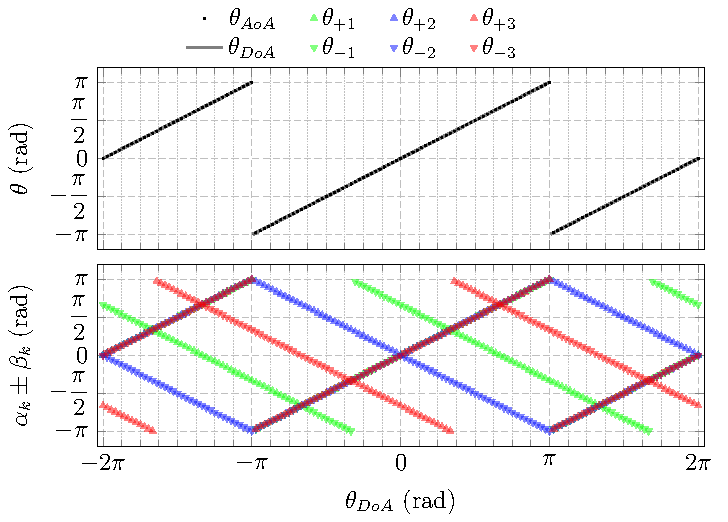
\includegraphics[height=0.785\textheight]{../pictures/simul_POLY_3_R_50.pdf}
			\caption*{\tiny Fonte: Autor, saída gráfica disponível em \href{https://github.com/HeckRodSav/TG/blob/main/documentation/pictures/POLY_3/simul_POLY_3_R_50.gif}{\underline{GitHub}}.}
		\end{figure}
	\end{frame}
	\begin{frame}
		\begin{figure}
			\centering
			\caption*{Caso $\text{SNR} = \SI{0}{\deci\bel}$, sem atenuação.}
			% \begin{tikzpicture}
    % \pgfsetfillopacity{0.5}

    \def\fileName{simul_POLY_3_R_50_SNR_1}
    \def\fileAddress{../../code/simul/Output/POLY_3/\fileName.dat}
	% \def\fileAddress{../data/\fileName.dat}

    \def\height{.25\linewidth}
    \def\width{0.75\linewidth}
    \def\distance{0.25cm}
    \def\xmin{-1}
    \def\xmax{101}

    \begin{axis} %configuração do eixo Y esquerdo e eixo X
    [
        name=plot1,
        reverse legend, % inverte a ordem que os items aparecem na legenda
    	% legend style={
        % 	at=(current bounding box.north),
        % 	anchor=south,
        % 	legend columns=6,
        % 	transpose legend,
        % 	draw=none,
        % 	/tikz/every even column/.append style={column sep=0.5cm}
    	% }, % onde exibir
        % axis x line=center,
        % axis y line=center,
        height=\height, % altura da região do gráfico
        width=\width, % largura da região do gráfico
        scale only axis, %
        minor grid style={densely dotted}, % estilo da grade secundária
        major grid style={densely dashed}, % estilo da grade principal
        grid style={lightgray, thin}, % cor das grades
        % axis on top, % forçar grade para ficar por cima do gráfico
        %
        %
        % axis y line*=left, % define gráfico para usar eixo esquerdo sem exibir direito
        y tick label style={
            /pgf/number format/.cd,
            fixed,
            % fixed zerofill,
            precision=1, % quantidade de casas depois da virgula
            /tikz/.cd
        },
        % y filter/.expression={y==0 ? NaN : y},
        scaled y ticks = false,
        ylabel={$\alpha_{k}\pm \beta_{k}$ (\si{\radian})}, % titulo eixo vertical
        % yticklabel={\pgfmathparse{\tick-50}\pgfmathprintnumber{\pgfmathresult}}, % fator multiplicativo para valores do eixo
        y tick label style={/pgf/number format/1000 sep=}, % Altera marcação de milhar
        % yticklabel style={rotate=90},
		ytick={-3.1415, -1.5708, 0, 1.5708, 3.1415},
		yticklabels={$-\pi$,$-\dfrac{\pi}{2}$,$0$,$\dfrac{\pi}{2}$,$\pi$},
        % ytick={0,1,2,3,4,5}, % lista de valores a serem utilizados no eixo
        % ymin=-1,  ymax=4,  % intervalo de valores no eixo y -> na dúvida, deixe comentado
        %
        ymajorgrids=true, % exibir grade principal y
        yminorgrids=true, % exibir grade secundária y
        minor y tick num=4, % contagem de linhas na grade secundária y
        % ybar,
        %
        %
        xlabel={$\theta_{DoA}$ (\si{\radian})}, % título eixo horizontal
        % xticklabel={\pgfmathparse{\tick-50}\pgfmathprintnumber{\pgfmathresult}}, % fator multiplicativo para valores do eixo
        % xticklabels={}, % fator multiplicativo para valores do eixo
		% xtick={0, 12.5, 25, 37.5, 50, 62.6, 75, 87.5, 100},
		% xticklabels={$-2~\pi$,$-\dfrac{3~\pi}{2}$,$-\pi$,$-\dfrac{\pi}{2}$,$0$,$-\dfrac{\pi}{2}$,$\pi$,$-\dfrac{3~\pi}{2}$,$2~\pi$},
		xtick={0, 25, 50, 75, 100},
		xticklabels={$-2 \pi$,$-\pi$,$0$,$\pi$,$2 \pi$},
        % xmode=log,
        % log ticks with fixed point,
        % x filter/.code=\pgfmathparse{#1 + 6.90775527898214},
        x tick label style={
            /pgf/number format/.cd,
            fixed,
            % fixed zerofill,
            precision=1,
            /tikz/.cd,
            /pgf/number format/use comma
        },
        xmin=\xmin, xmax=\xmax, % intervalo de valores no eixo x -> na dúvida, deixe comentado
        scaled x ticks = false,
        %
        xmajorgrids=true, % exibir grade principal x
        xminorgrids=true, % exibir grade secundária x
        minor x tick num=7, % contagem de linhas na grade secundária x
        %
        %
        %
        % unbounded coords=jump,
        % jump threshold/.initial=0.25
    ]

	\addplot[
        cmyk_G,
        mark=triangle*,
		opacity=0.5,
        only marks,
        % smooth
    ] table [
        % col sep=comma,
        x=percent, % cabeçalho da coluna de dados X no arquivo
        y=delta_1_x_3, % cabeçalho da coluna de dados Y no arquivo
    ]
    {\fileAddress};	\label{\fileName.1.1}

    \addplot[
        cmyk_G,
        mark=triangle*,
		opacity=0.5,
		mark options={rotate=180},
        only marks,
        % smooth
    ] table [
        % col sep=comma,
        x=percent, % cabeçalho da coluna de dados X no arquivo
        y=delta_3_x_1, % cabeçalho da coluna de dados Y no arquivo
    ]
    {\fileAddress};	\label{\fileName.1.2}

	\addplot[
        cmyk_B,
        mark=triangle*,
		opacity=0.5,
        only marks,
        % smooth
    ] table [
        % col sep=comma,
        x=percent, % cabeçalho da coluna de dados X no arquivo
        y=delta_2_x_1, % cabeçalho da coluna de dados Y no arquivo
    ]
    {\fileAddress};	\label{\fileName.1.3}

    \addplot[
        cmyk_B,
        mark=triangle*,
		opacity=0.5,
		mark options={rotate=180},
        only marks,
        % smooth
    ] table [
        % col sep=comma,
        x=percent, % cabeçalho da coluna de dados X no arquivo
        y=delta_1_x_2, % cabeçalho da coluna de dados Y no arquivo
    ]
    {\fileAddress};	\label{\fileName.1.4}

	\addplot[
        cmyk_R,
        mark=triangle*,
		opacity=0.5,
        only marks,
        % smooth
    ] table [
        % col sep=comma,
        x=percent, % cabeçalho da coluna de dados X no arquivo
        y=delta_3_x_2, % cabeçalho da coluna de dados Y no arquivo
    ]
    {\fileAddress};	\label{\fileName.1.5}

    \addplot[
        cmyk_R,
        mark=triangle*,
		opacity=0.5,
		mark options={rotate=180},
        only marks,
        % smooth
    ] table [
        % col sep=comma,
        x=percent, % cabeçalho da coluna de dados X no arquivo
        y=delta_2_x_3, % cabeçalho da coluna de dados Y no arquivo
    ]
    {\fileAddress};	\label{\fileName.1.6}

    \end{axis}

    % \begin{axis} %configuração do eixo Y direito e legenda
    % [
    %     legend cell align=left, % alinhamento de texto na legenda
    %     % legend pos={outer north east}, % onde exibir caixa de legenda
    %     % reverse legend, % inverte a ordem que os items aparecem na legenda
    % 	legend style={
    %     	at=(current bounding box.north),
    %     	anchor=south,
    %     	legend columns=2,
    %     % 	transpose legend,
    %     	draw=none
    % 	}, % onde exibir
    %     % axis x line=center,
    %     % axis y line=center,
    %     height=\height, % altura da região do gráfico
    %     width=\width, % largura da região do gráfico
    %     scale only axis, %
    %     minor grid style={densely dotted}, % estilo da grade secundária
    %     major grid style={densely dashed}, % estilo da grade principal
    %     grid style={lightgray, thin}, % cor das grades
    %     % axis on top, % forçar grade para ficar por cima do gráfico
    %     %
    %     %
    %     axis y line*=right, % define gráfico para usar eixo direito sem exibir esquerdo
    %     ylabel={$V_{out}$ (\si{\milli\volt})}, % titulo eixo vertical
    %     y tick label style={
    %         /pgf/number format/.cd,
    %         fixed,
    %         % fixed zerofill,
    %         precision=3, % quantidade de casas depois da virgula
    %         /tikz/.cd,
    %         /pgf/number format/use comma
    %     },
    %     % y filter/.expression={y==0 ? NaN : y},
    %     scaled y ticks = false,
    %     % yticklabel={\pgfmathparse{\tick*10^3}\pgfmathprintnumber{\pgfmathresult}}, % fator multiplicativo para valores do eixo
    %     y tick label style={/pgf/number format/1000 sep=}, % Altera marcação de milhar
    %     % yticklabel style={rotate=90},
    %     % ytick={-12,-6,0,6,12}, % lista de valores a serem utilizados no eixo
    %     % ymin=0.76503, ymax=0.76509,  % intervalo de valores no eixo y -> na dúvida, deixe comentado
    %     %
    %     ymajorgrids=false, % exibir grade principal y
    %     yminorgrids=false, % exibir grade secundária y
    %     minor y tick num=4, % contagem de linhas na grade secundária y
    %     % ybar,
    %     %
    %     %
    %     axis x line=none, %oculta eixo inferior quando o gráfico anterior já exibe
    %     % xlabel={Frequência (\si{\hertz})}, % título eixo horizontal
    %     % xticklabel={\pgfmathparse{\tick*10^3}\pgfmathprintnumber{\pgfmathresult}}, % fator multiplicativo para valores do eixo
    %     % xmode=log,
    %     % log ticks with fixed point,
    %     % x filter/.code=\pgfmathparse{#1 + 6.90775527898214},
    %     % x tick label style={
    %     %     /pgf/number format/.cd,
    %     %     fixed,
    %     %     % fixed zerofill,
    %     %     precision=0,
    %     %     /tikz/.cd,
    %     %     /pgf/number format/use comma
    %     % },
    %     xmin=\xmin, xmax=\xmax, % intervalo de valores no eixo x -> na dúvida, deixe comentado
    %     % scaled x ticks = true,
    %     %
    %     % xmajorgrids=true, % exibir grade principal x
    %     % xminorgrids=true, % exibir grade secundária x
    %     % minor x tick num=7, % contagem de linhas na grade secundária x
    %     %
    %     %
    %     %
    % ]



    % \addplot[mark=none,red, thick]
    % table [
    %     x=time, % cabeçalho da coluna de dados X no arquivo
    %     y=vout % cabeçalho da coluna de dados Y no arquivo
    % ]
    % {graficos/dados/booster.dat};  \label{\fileName.1.2}

    % % \addlegendimage{/pgfplots/refstyle=_1_2}

    % % \addplot[ForestGreen, densely dashdotted, thick]
    % % coordinates
    % % {
    % %     (\pgfkeysvalueof{/pgfplots/xmin},12)
    % %     (\pgfkeysvalueof{/pgfplots/xmax},12)
    % % };
    % % % \addlegendentry{$V_{out}=\pm\SI{12}{\volt}$}

    % % \addplot[ForestGreen, densely dashdotted, thick]
    % % coordinates
    % % {
    % %     (\pgfkeysvalueof{/pgfplots/xmin},-12)
    % %     (\pgfkeysvalueof{/pgfplots/xmax},-12)
    % % };

    % \end{axis}

    \begin{axis} %configuração do eixo Y esquerdo e eixo X
    [
        at={($(plot1.north)+(0,\distance)$)},
        anchor=south,
        % reverse legend, % inverte a ordem que os items aparecem na legenda
		legend style={
        	at=(current bounding box.north),
        	anchor=south,
        	legend columns=2,
        	transpose legend,
        	draw=none,
        	/tikz/every even column/.append style={column sep=0.5cm}
    	}, % onde exibir
        samples=505,
        domain=0:100,
        % axis x line=center,
        % axis y line=center,
        height=\height, % altura da região do gráfico
        width=\width, % largura da região do gráfico
        scale only axis, %
        minor grid style={densely dotted}, % estilo da grade secundária
        major grid style={densely dashed}, % estilo da grade principal
        grid style={lightgray, thin}, % cor das grades
        % axis on top, % forçar grade para ficar por cima do gráfico
        %
        %
        % axis y line*=left, % define gráfico para usar eixo esquerdo sem exibir direito
        y tick label style={
            /pgf/number format/.cd,
            fixed,
            % fixed zerofill,
            precision=1, % quantidade de casas depois da virgula
            /tikz/.cd
        },
        % y filter/.expression={y==0 ? NaN : y},
        scaled y ticks = false,
        ylabel={$\theta$ (\si{\radian})}, % titulo eixo vertical
        % yticklabel={\pgfmathparse{\tick*10^3}\pgfmathprintnumber{\pgfmathresult}}, % fator multiplicativo para valores do eixo
        y tick label style={/pgf/number format/1000 sep=}, % Altera marcação de milhar
        % yticklabel style={rotate=90},
		ytick={-3.1415, -1.5708, 0, 1.5708, 3.1415},
		yticklabels={$-\pi$,$-\dfrac{\pi}{2}$,$0$,$\dfrac{\pi}{2}$,$\pi$},
        % ytick={0,1,2,3,4,5}, % lista de valores a serem utilizados no eixo
        % ymin=-1,  ymax=4,  % intervalo de valores no eixo y -> na dúvida, deixe comentado
        %
        ymajorgrids=true, % exibir grade principal y
        yminorgrids=true, % exibir grade secundária y
        minor y tick num=4, % contagem de linhas na grade secundária y
        % ybar,
        %
        %
        % xlabel={Tempo (\si{\milli\second})}, % título eixo horizontal
        % xticklabel={\pgfmathparse{\tick*10^3}\pgfmathprintnumber{\pgfmathresult}}, % fator multiplicativo para valores do eixo
		xtick={0, 25, 50, 75, 100},
        xticklabels={}, % fator multiplicativo para valores do eixo
        % xmode=log,
        % log ticks with fixed point,
        % x filter/.code=\pgfmathparse{#1 + 6.90775527898214},
        x tick label style={
            /pgf/number format/.cd,
            fixed,
            % fixed zerofill,
            precision=1,
            /tikz/.cd,
            /pgf/number format/use comma
        },
        xmin=\xmin, xmax=\xmax, % intervalo de valores no eixo x -> na dúvida, deixe comentado
        scaled x ticks = false,
        %
        xmajorgrids=true, % exibir grade principal x
        xminorgrids=true, % exibir grade secundária x
        minor x tick num=7, % contagem de linhas na grade secundária x
        %
        %
        %
        unbounded coords=jump,
		jump threshold/.initial=0.01
    ]


    \addplot[
        Black,
        mark=*,
		mark size=0.5pt,
        only marks,
        % smooth
    ] table [
        % col sep=comma,
        x=percent, % cabeçalho da coluna de dados X no arquivo
        y=choose_angle, % cabeçalho da coluna de dados Y no arquivo
	]
	{\fileAddress};	\addlegendentry{$\theta_{AoA}$}

	% \addplot[
	% 	Black,
	% 	mark=o,
	% 	mark size=1.5pt,
	% 	only marks,
	% 	opacity=0.5,
    %     thick,
	% 	% smooth
	% ] table [
	% 	% col sep=comma,
	% 	x=percent, % cabeçalho da coluna de dados X no arquivo
	% 	y=ang_W, % cabeçalho da coluna de dados Y no arquivo
	% ]
	% {\fileAddress};
    \addplot [
        Black,
        opacity=0.5,
        mark=none,
        mark size=5pt,
        very thick,
        % only marks,
        % smooth
    ] {((x==25)||(x==75)?nan:pi*(mod(x+25,50)-25)/25)};
    \addlegendentry{$\theta_{DoA}$}


	\addlegendimage{/pgfplots/refstyle=\fileName.1.1}\addlegendentry{$\theta_{+1}$}
	\addlegendimage{/pgfplots/refstyle=\fileName.1.2}\addlegendentry{$\theta_{-1}$}

	\addlegendimage{/pgfplots/refstyle=\fileName.1.3}\addlegendentry{$\theta_{+2}$}
	\addlegendimage{/pgfplots/refstyle=\fileName.1.4}\addlegendentry{$\theta_{-2}$}

    \addlegendimage{/pgfplots/refstyle=\fileName.1.5}\addlegendentry{$\theta_{+3}$}
	\addlegendimage{/pgfplots/refstyle=\fileName.1.6}\addlegendentry{$\theta_{-3}$}

    \end{axis}

    % \begin{axis} %configuração do eixo Y direito e legenda
    % [
    %     at={($(plot1.north)+(0,\distance)$)},
    %     anchor=south,
    %     legend cell align=left, % alinhamento de texto na legenda
    %     % legend pos={outer north east}, % onde exibir caixa de legenda
    %     % reverse legend, % inverte a ordem que os items aparecem na legenda
    % 	legend style={
    %     	at=(current bounding box.north),
    %     	anchor=south,
    %     	legend columns=3,
    %     % 	transpose legend,
    %     	draw=none,
    %     	/tikz/every even column/.append style={column sep=0.5cm}
    % 	}, % onde exibir
    %     % axis x line=center,
    %     % axis y line=center,
    %     height=\height, % altura da região do gráfico
    %     width=\width, % largura da região do gráfico
    %     scale only axis, %
    %     minor grid style={densely dotted}, % estilo da grade secundária
    %     major grid style={densely dashed}, % estilo da grade principal
    %     grid style={lightgray, thin}, % cor das grades
    %     % axis on top, % forçar grade para ficar por cima do gráfico
    %     %
    %     %
    %     axis y line*=right, % define gráfico para usar eixo direito sem exibir esquerdo
    %     ylabel={$V_{out}$ (\si{\volt})}, % titulo eixo vertical
    %     y tick label style={
    %         /pgf/number format/.cd,
    %         fixed,
    %         % fixed zerofill,
    %         precision=3, % quantidade de casas depois da virgula
    %         /tikz/.cd,
    %         /pgf/number format/use comma
    %     },
    %     % y filter/.expression={y==0 ? NaN : y},
    %     scaled y ticks = false,
    %     % yticklabel={\pgfmathparse{\tick*10^3}\pgfmathprintnumber{\pgfmathresult}}, % fator multiplicativo para valores do eixo
    %     y tick label style={/pgf/number format/1000 sep=}, % Altera marcação de milhar
    %     % yticklabel style={rotate=90},
    %     % ytick={-12,-6,0,6,12}, % lista de valores a serem utilizados no eixo
    %     % ymin=0.76503, ymax=0.76509,  % intervalo de valores no eixo y -> na dúvida, deixe comentado
    %     %
    %     ymajorgrids=false, % exibir grade principal y
    %     yminorgrids=false, % exibir grade secundária y
    %     minor y tick num=4, % contagem de linhas na grade secundária y
    %     % ybar,
    %     %
    %     %
    %     axis x line=none, %oculta eixo inferior quando o gráfico anterior já exibe
    %     % xlabel={Frequência (\si{\hertz})}, % título eixo horizontal
    %     % xticklabel={\pgfmathparse{\tick*10^3}\pgfmathprintnumber{\pgfmathresult}}, % fator multiplicativo para valores do eixo
    %     % xmode=log,
    %     % log ticks with fixed point,
    %     % x filter/.code=\pgfmathparse{#1 + 6.90775527898214},
    %     % x tick label style={
    %     %     /pgf/number format/.cd,
    %     %     fixed,
    %     %     % fixed zerofill,
    %     %     precision=0,
    %     %     /tikz/.cd,
    %     %     /pgf/number format/use comma
    %     % },
    %     xmin=\xmin, xmax=\xmax, % intervalo de valores no eixo x -> na dúvida, deixe comentado
    %     % scaled x ticks = true,
    %     %
    %     % xmajorgrids=true, % exibir grade principal x
    %     % xminorgrids=true, % exibir grade secundária x
    %     % minor x tick num=10, % contagem de linhas na grade secundária x
    %     %
    %     %
    %     %
    % ]


    % \addlegendimage{/pgfplots/refstyle=_2_1}\addlegendentry{$V_{in}$}
    % \addlegendimage{/pgfplots/refstyle=_2_2}\addlegendentry{$V_{in}$}
    % % \addplot[mark=none,red, thick]
    % % table [
    % %     x=time, % cabeçalho da coluna de dados X no arquivo
    % %     y=vout % cabeçalho da coluna de dados Y no arquivo
    % % ]
    % % {graficos/dados/booster.dat}; % \label{\fileName.1.2}
    % % \addlegendentry{$V_{out}$}

    % \addlegendimage{/pgfplots/refstyle=_1_1}\addlegendentry{$I_{out}$}
    % \addlegendimage{/pgfplots/refstyle=_1_2}\addlegendentry{$I_{out}$}

    % % \addlegendimage{/pgfplots/refstyle=_1_2}

    % % \addplot[ForestGreen, densely dashdotted, thick]
    % % coordinates
    % % {
    % %     (\pgfkeysvalueof{/pgfplots/xmin},12)
    % %     (\pgfkeysvalueof{/pgfplots/xmax},12)
    % % };
    % % % \addlegendentry{$V_{out}=\pm\SI{12}{\volt}$}

    % % \addplot[ForestGreen, densely dashdotted, thick]
    % % coordinates
    % % {
    % %     (\pgfkeysvalueof{/pgfplots/xmin},-12)
    % %     (\pgfkeysvalueof{/pgfplots/xmax},-12)
    % % };

    % \end{axis}



\end{tikzpicture}

			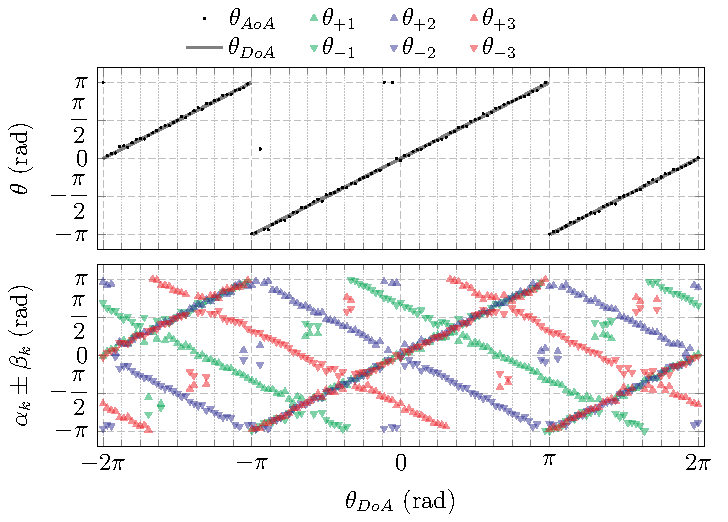
\includegraphics[height=0.785\textheight]{../pictures/simul_POLY_3_R_50_SNR_1.pdf}
			\caption*{\tiny Fonte: Autor, saída gráfica disponível em \href{https://github.com/HeckRodSav/TG/blob/main/documentation/pictures/POLY_3/simul_POLY_3_R_50_SNR_1.gif}{\underline{GitHub}}.}
		\end{figure}
	\end{frame}
	\begin{frame}
		\begin{figure}
			\centering
			\caption*{Caso $\text{SNR} = \SI{0}{\deci\bel}$, com atenuação.}
			% \begin{tikzpicture}
    % \pgfsetfillopacity{0.5}

    \def\fileName{simul_POLY_3_R_50_SNR_1_ATT}
    % \def\fileAddress{../../code/simul/Output/POLY_3/\fileName.dat}
    \def\fileAddress{../data/POLY_3/\fileName.dat}
    % \def\fileAddress{../data/\fileName.dat}

    \def\height{.225\linewidth}
    \def\width{0.75\linewidth}
    \def\distance{0.25cm}
    \def\xmin{-1}
    \def\xmax{101}

    \begin{axis} %configuração do eixo Y esquerdo e eixo X
    [
        name=plot1,
        reverse legend, % inverte a ordem que os items aparecem na legenda
    	% legend style={
        % 	at=(current bounding box.north),
        % 	anchor=south,
        % 	legend columns=6,
        % 	transpose legend,
        % 	draw=none,
        % 	/tikz/every even column/.append style={column sep=0.5cm}
    	% }, % onde exibir
        % axis x line=center,
        % axis y line=center,
        height=\height, % altura da região do gráfico
        width=\width, % largura da região do gráfico
        scale only axis, %
        minor grid style={densely dotted}, % estilo da grade secundária
        major grid style={densely dashed}, % estilo da grade principal
        grid style={lightgray, thin}, % cor das grades
        % axis on top, % forçar grade para ficar por cima do gráfico
        %
        %
        % axis y line*=left, % define gráfico para usar eixo esquerdo sem exibir direito
        y tick label style={
            /pgf/number format/.cd,
            fixed,
            % fixed zerofill,
            precision=1, % quantidade de casas depois da virgula
            /tikz/.cd
        },
        % y filter/.expression={y==0 ? NaN : y},
        scaled y ticks = false,
        ylabel={$\alpha_{k}\pm \beta_{k}$ (\si{\radian})}, % titulo eixo vertical
        % yticklabel={\pgfmathparse{\tick-50}\pgfmathprintnumber{\pgfmathresult}}, % fator multiplicativo para valores do eixo
        y tick label style={/pgf/number format/1000 sep=}, % Altera marcação de milhar
        % yticklabel style={rotate=90},
		ytick={-3.1415, -1.5708, 0, 1.5708, 3.1415},
		yticklabels={$-\pi$,$-\dfrac{\pi}{2}$,$0$,$\dfrac{\pi}{2}$,$\pi$},
        % ytick={0,1,2,3,4,5}, % lista de valores a serem utilizados no eixo
        % ymin=-1,  ymax=4,  % intervalo de valores no eixo y -> na dúvida, deixe comentado
        %
        ymajorgrids=true, % exibir grade principal y
        yminorgrids=true, % exibir grade secundária y
        minor y tick num=4, % contagem de linhas na grade secundária y
        % ybar,
        %
        %
        xlabel={$\theta_{DoA}$ (\si{\radian})}, % título eixo horizontal
        % xticklabel={\pgfmathparse{\tick-50}\pgfmathprintnumber{\pgfmathresult}}, % fator multiplicativo para valores do eixo
        % xticklabels={}, % fator multiplicativo para valores do eixo
		% xtick={0, 12.5, 25, 37.5, 50, 62.6, 75, 87.5, 100},
		% xticklabels={$-2~\pi$,$-\dfrac{3~\pi}{2}$,$-\pi$,$-\dfrac{\pi}{2}$,$0$,$-\dfrac{\pi}{2}$,$\pi$,$-\dfrac{3~\pi}{2}$,$2~\pi$},
		xtick={0, 25, 50, 75, 100},
		xticklabels={$-2 \pi$,$-\pi$,$0$,$\pi$,$2 \pi$},
        % xmode=log,
        % log ticks with fixed point,
        % x filter/.code=\pgfmathparse{#1 + 6.90775527898214},
        x tick label style={
            /pgf/number format/.cd,
            fixed,
            % fixed zerofill,
            precision=1,
            /tikz/.cd,
            /pgf/number format/use comma
        },
        xmin=\xmin, xmax=\xmax, % intervalo de valores no eixo x -> na dúvida, deixe comentado
        scaled x ticks = false,
        %
        xmajorgrids=true, % exibir grade principal x
        xminorgrids=true, % exibir grade secundária x
        minor x tick num=7, % contagem de linhas na grade secundária x
        %
        %
        %
        % unbounded coords=jump,
        % jump threshold/.initial=0.25
    ]

	\addplot[
        antena_3_1,
        mark=triangle*,
		opacity=0.5,
        only marks,
        % smooth
    ] table [
        % col sep=comma,
        x=percent, % cabeçalho da coluna de dados X no arquivo
        y=delta_1_x_3, % cabeçalho da coluna de dados Y no arquivo
    ]
    {\fileAddress};	\label{\fileName.1.1}

    \addplot[
        antena_3_1,
        mark=triangle*,
		opacity=0.5,
		mark options={rotate=180},
        only marks,
        % smooth
    ] table [
        % col sep=comma,
        x=percent, % cabeçalho da coluna de dados X no arquivo
        y=delta_3_x_1, % cabeçalho da coluna de dados Y no arquivo
    ]
    {\fileAddress};	\label{\fileName.1.2}

	\addplot[
        antena_3_2,
        mark=triangle*,
		opacity=0.5,
        only marks,
        % smooth
    ] table [
        % col sep=comma,
        x=percent, % cabeçalho da coluna de dados X no arquivo
        y=delta_2_x_1, % cabeçalho da coluna de dados Y no arquivo
    ]
    {\fileAddress};	\label{\fileName.1.3}

    \addplot[
        antena_3_2,
        mark=triangle*,
		opacity=0.5,
		mark options={rotate=180},
        only marks,
        % smooth
    ] table [
        % col sep=comma,
        x=percent, % cabeçalho da coluna de dados X no arquivo
        y=delta_1_x_2, % cabeçalho da coluna de dados Y no arquivo
    ]
    {\fileAddress};	\label{\fileName.1.4}

	\addplot[
        antena_3_3,
        mark=triangle*,
		opacity=0.5,
        only marks,
        % smooth
    ] table [
        % col sep=comma,
        x=percent, % cabeçalho da coluna de dados X no arquivo
        y=delta_3_x_2, % cabeçalho da coluna de dados Y no arquivo
    ]
    {\fileAddress};	\label{\fileName.1.5}

    \addplot[
        antena_3_3,
        mark=triangle*,
		opacity=0.5,
		mark options={rotate=180},
        only marks,
        % smooth
    ] table [
        % col sep=comma,
        x=percent, % cabeçalho da coluna de dados X no arquivo
        y=delta_2_x_3, % cabeçalho da coluna de dados Y no arquivo
    ]
    {\fileAddress};	\label{\fileName.1.6}

    \end{axis}

    % \begin{axis} %configuração do eixo Y direito e legenda
    % [
    %     legend cell align=left, % alinhamento de texto na legenda
    %     % legend pos={outer north east}, % onde exibir caixa de legenda
    %     % reverse legend, % inverte a ordem que os items aparecem na legenda
    % 	legend style={
    %     	at=(current bounding box.north),
    %     	anchor=south,
    %     	legend columns=2,
    %     % 	transpose legend,
    %     	draw=none
    % 	}, % onde exibir
    %     % axis x line=center,
    %     % axis y line=center,
    %     height=\height, % altura da região do gráfico
    %     width=\width, % largura da região do gráfico
    %     scale only axis, %
    %     minor grid style={densely dotted}, % estilo da grade secundária
    %     major grid style={densely dashed}, % estilo da grade principal
    %     grid style={lightgray, thin}, % cor das grades
    %     % axis on top, % forçar grade para ficar por cima do gráfico
    %     %
    %     %
    %     axis y line*=right, % define gráfico para usar eixo direito sem exibir esquerdo
    %     ylabel={$V_{out}$ (\si{\milli\volt})}, % titulo eixo vertical
    %     y tick label style={
    %         /pgf/number format/.cd,
    %         fixed,
    %         % fixed zerofill,
    %         precision=3, % quantidade de casas depois da virgula
    %         /tikz/.cd,
    %         /pgf/number format/use comma
    %     },
    %     % y filter/.expression={y==0 ? NaN : y},
    %     scaled y ticks = false,
    %     % yticklabel={\pgfmathparse{\tick*10^3}\pgfmathprintnumber{\pgfmathresult}}, % fator multiplicativo para valores do eixo
    %     y tick label style={/pgf/number format/1000 sep=}, % Altera marcação de milhar
    %     % yticklabel style={rotate=90},
    %     % ytick={-12,-6,0,6,12}, % lista de valores a serem utilizados no eixo
    %     % ymin=0.76503, ymax=0.76509,  % intervalo de valores no eixo y -> na dúvida, deixe comentado
    %     %
    %     ymajorgrids=false, % exibir grade principal y
    %     yminorgrids=false, % exibir grade secundária y
    %     minor y tick num=4, % contagem de linhas na grade secundária y
    %     % ybar,
    %     %
    %     %
    %     axis x line=none, %oculta eixo inferior quando o gráfico anterior já exibe
    %     % xlabel={Frequência (\si{\hertz})}, % título eixo horizontal
    %     % xticklabel={\pgfmathparse{\tick*10^3}\pgfmathprintnumber{\pgfmathresult}}, % fator multiplicativo para valores do eixo
    %     % xmode=log,
    %     % log ticks with fixed point,
    %     % x filter/.code=\pgfmathparse{#1 + 6.90775527898214},
    %     % x tick label style={
    %     %     /pgf/number format/.cd,
    %     %     fixed,
    %     %     % fixed zerofill,
    %     %     precision=0,
    %     %     /tikz/.cd,
    %     %     /pgf/number format/use comma
    %     % },
    %     xmin=\xmin, xmax=\xmax, % intervalo de valores no eixo x -> na dúvida, deixe comentado
    %     % scaled x ticks = true,
    %     %
    %     % xmajorgrids=true, % exibir grade principal x
    %     % xminorgrids=true, % exibir grade secundária x
    %     % minor x tick num=7, % contagem de linhas na grade secundária x
    %     %
    %     %
    %     %
    % ]



    % \addplot[mark=none,red, thick]
    % table [
    %     x=time, % cabeçalho da coluna de dados X no arquivo
    %     y=vout % cabeçalho da coluna de dados Y no arquivo
    % ]
    % {graficos/dados/booster.dat};  \label{\fileName.1.2}

    % % \addlegendimage{/pgfplots/refstyle=_1_2}

    % % \addplot[ForestGreen, densely dashdotted, thick]
    % % coordinates
    % % {
    % %     (\pgfkeysvalueof{/pgfplots/xmin},12)
    % %     (\pgfkeysvalueof{/pgfplots/xmax},12)
    % % };
    % % % \addlegendentry{$V_{out}=\pm\SI{12}{\volt}$}

    % % \addplot[ForestGreen, densely dashdotted, thick]
    % % coordinates
    % % {
    % %     (\pgfkeysvalueof{/pgfplots/xmin},-12)
    % %     (\pgfkeysvalueof{/pgfplots/xmax},-12)
    % % };

    % \end{axis}

    \begin{axis} %configuração do eixo Y esquerdo e eixo X
    [
        at={($(plot1.north)+(0,\distance)$)},
        anchor=south,
        % reverse legend, % inverte a ordem que os items aparecem na legenda
		legend style={
        	at=(current bounding box.north),
        	anchor=south,
        	legend columns=2,
        	transpose legend,
        	draw=none,
        	/tikz/every even column/.append style={column sep=0.5cm}
    	}, % onde exibir
        samples=505,
        domain=0:100,
        % axis x line=center,
        % axis y line=center,
        height=\height, % altura da região do gráfico
        width=\width, % largura da região do gráfico
        scale only axis, %
        minor grid style={densely dotted}, % estilo da grade secundária
        major grid style={densely dashed}, % estilo da grade principal
        grid style={lightgray, thin}, % cor das grades
        % axis on top, % forçar grade para ficar por cima do gráfico
        %
        %
        % axis y line*=left, % define gráfico para usar eixo esquerdo sem exibir direito
        y tick label style={
            /pgf/number format/.cd,
            fixed,
            % fixed zerofill,
            precision=1, % quantidade de casas depois da virgula
            /tikz/.cd
        },
        % y filter/.expression={y==0 ? NaN : y},
        scaled y ticks = false,
        ylabel={$\theta$ (\si{\radian})}, % titulo eixo vertical
        % yticklabel={\pgfmathparse{\tick*10^3}\pgfmathprintnumber{\pgfmathresult}}, % fator multiplicativo para valores do eixo
        y tick label style={/pgf/number format/1000 sep=}, % Altera marcação de milhar
        % yticklabel style={rotate=90},
		ytick={-3.1415, -1.5708, 0, 1.5708, 3.1415},
		yticklabels={$-\pi$,$-\dfrac{\pi}{2}$,$0$,$\dfrac{\pi}{2}$,$\pi$},
        % ytick={0,1,2,3,4,5}, % lista de valores a serem utilizados no eixo
        % ymin=-1,  ymax=4,  % intervalo de valores no eixo y -> na dúvida, deixe comentado
        %
        ymajorgrids=true, % exibir grade principal y
        yminorgrids=true, % exibir grade secundária y
        minor y tick num=4, % contagem de linhas na grade secundária y
        % ybar,
        %
        %
        % xlabel={Tempo (\si{\milli\second})}, % título eixo horizontal
        % xticklabel={\pgfmathparse{\tick*10^3}\pgfmathprintnumber{\pgfmathresult}}, % fator multiplicativo para valores do eixo
		xtick={0, 25, 50, 75, 100},
        xticklabels={}, % fator multiplicativo para valores do eixo
        % xmode=log,
        % log ticks with fixed point,
        % x filter/.code=\pgfmathparse{#1 + 6.90775527898214},
        x tick label style={
            /pgf/number format/.cd,
            fixed,
            % fixed zerofill,
            precision=1,
            /tikz/.cd,
            /pgf/number format/use comma
        },
        xmin=\xmin, xmax=\xmax, % intervalo de valores no eixo x -> na dúvida, deixe comentado
        scaled x ticks = false,
        %
        xmajorgrids=true, % exibir grade principal x
        xminorgrids=true, % exibir grade secundária x
        minor x tick num=7, % contagem de linhas na grade secundária x
        %
        %
        %
        unbounded coords=jump,
		jump threshold/.initial=0.01
    ]


    \addplot[
        Black,
        mark=*,
		mark size=0.5pt,
        only marks,
        % smooth
    ] table [
        % col sep=comma,
        x=percent, % cabeçalho da coluna de dados X no arquivo
        y=choose_angle, % cabeçalho da coluna de dados Y no arquivo
	]
	{\fileAddress};	\addlegendentry{$\theta_{AoA}$}

	% \addplot[
	% 	Black,
	% 	mark=o,
	% 	mark size=1.5pt,
	% 	only marks,
	% 	opacity=0.5,
    %     thick,
	% 	% smooth
	% ] table [
	% 	% col sep=comma,
	% 	x=percent, % cabeçalho da coluna de dados X no arquivo
	% 	y=ang_W, % cabeçalho da coluna de dados Y no arquivo
	% ]
	% {\fileAddress};
    \addplot [
        Black,
        opacity=0.5,
        mark=none,
        mark size=5pt,
        very thick,
        % only marks,
        % smooth
    ] {((x==25)||(x==75)?nan:pi*(mod(x+25,50)-25)/25)};
    \addlegendentry{$\theta_{DoA}$}


	\addlegendimage{/pgfplots/refstyle=\fileName.1.1}\addlegendentry{$\theta_{+1}$}
	\addlegendimage{/pgfplots/refstyle=\fileName.1.2}\addlegendentry{$\theta_{-1}$}

	\addlegendimage{/pgfplots/refstyle=\fileName.1.3}\addlegendentry{$\theta_{+2}$}
	\addlegendimage{/pgfplots/refstyle=\fileName.1.4}\addlegendentry{$\theta_{-2}$}

    \addlegendimage{/pgfplots/refstyle=\fileName.1.5}\addlegendentry{$\theta_{+3}$}
	\addlegendimage{/pgfplots/refstyle=\fileName.1.6}\addlegendentry{$\theta_{-3}$}

    \end{axis}

    % \begin{axis} %configuração do eixo Y direito e legenda
    % [
    %     at={($(plot1.north)+(0,\distance)$)},
    %     anchor=south,
    %     legend cell align=left, % alinhamento de texto na legenda
    %     % legend pos={outer north east}, % onde exibir caixa de legenda
    %     % reverse legend, % inverte a ordem que os items aparecem na legenda
    % 	legend style={
    %     	at=(current bounding box.north),
    %     	anchor=south,
    %     	legend columns=3,
    %     % 	transpose legend,
    %     	draw=none,
    %     	/tikz/every even column/.append style={column sep=0.5cm}
    % 	}, % onde exibir
    %     % axis x line=center,
    %     % axis y line=center,
    %     height=\height, % altura da região do gráfico
    %     width=\width, % largura da região do gráfico
    %     scale only axis, %
    %     minor grid style={densely dotted}, % estilo da grade secundária
    %     major grid style={densely dashed}, % estilo da grade principal
    %     grid style={lightgray, thin}, % cor das grades
    %     % axis on top, % forçar grade para ficar por cima do gráfico
    %     %
    %     %
    %     axis y line*=right, % define gráfico para usar eixo direito sem exibir esquerdo
    %     ylabel={$V_{out}$ (\si{\volt})}, % titulo eixo vertical
    %     y tick label style={
    %         /pgf/number format/.cd,
    %         fixed,
    %         % fixed zerofill,
    %         precision=3, % quantidade de casas depois da virgula
    %         /tikz/.cd,
    %         /pgf/number format/use comma
    %     },
    %     % y filter/.expression={y==0 ? NaN : y},
    %     scaled y ticks = false,
    %     % yticklabel={\pgfmathparse{\tick*10^3}\pgfmathprintnumber{\pgfmathresult}}, % fator multiplicativo para valores do eixo
    %     y tick label style={/pgf/number format/1000 sep=}, % Altera marcação de milhar
    %     % yticklabel style={rotate=90},
    %     % ytick={-12,-6,0,6,12}, % lista de valores a serem utilizados no eixo
    %     % ymin=0.76503, ymax=0.76509,  % intervalo de valores no eixo y -> na dúvida, deixe comentado
    %     %
    %     ymajorgrids=false, % exibir grade principal y
    %     yminorgrids=false, % exibir grade secundária y
    %     minor y tick num=4, % contagem de linhas na grade secundária y
    %     % ybar,
    %     %
    %     %
    %     axis x line=none, %oculta eixo inferior quando o gráfico anterior já exibe
    %     % xlabel={Frequência (\si{\hertz})}, % título eixo horizontal
    %     % xticklabel={\pgfmathparse{\tick*10^3}\pgfmathprintnumber{\pgfmathresult}}, % fator multiplicativo para valores do eixo
    %     % xmode=log,
    %     % log ticks with fixed point,
    %     % x filter/.code=\pgfmathparse{#1 + 6.90775527898214},
    %     % x tick label style={
    %     %     /pgf/number format/.cd,
    %     %     fixed,
    %     %     % fixed zerofill,
    %     %     precision=0,
    %     %     /tikz/.cd,
    %     %     /pgf/number format/use comma
    %     % },
    %     xmin=\xmin, xmax=\xmax, % intervalo de valores no eixo x -> na dúvida, deixe comentado
    %     % scaled x ticks = true,
    %     %
    %     % xmajorgrids=true, % exibir grade principal x
    %     % xminorgrids=true, % exibir grade secundária x
    %     % minor x tick num=10, % contagem de linhas na grade secundária x
    %     %
    %     %
    %     %
    % ]


    % \addlegendimage{/pgfplots/refstyle=_2_1}\addlegendentry{$V_{in}$}
    % \addlegendimage{/pgfplots/refstyle=_2_2}\addlegendentry{$V_{in}$}
    % % \addplot[mark=none,red, thick]
    % % table [
    % %     x=time, % cabeçalho da coluna de dados X no arquivo
    % %     y=vout % cabeçalho da coluna de dados Y no arquivo
    % % ]
    % % {graficos/dados/booster.dat}; % \label{\fileName.1.2}
    % % \addlegendentry{$V_{out}$}

    % \addlegendimage{/pgfplots/refstyle=_1_1}\addlegendentry{$I_{out}$}
    % \addlegendimage{/pgfplots/refstyle=_1_2}\addlegendentry{$I_{out}$}

    % % \addlegendimage{/pgfplots/refstyle=_1_2}

    % % \addplot[ForestGreen, densely dashdotted, thick]
    % % coordinates
    % % {
    % %     (\pgfkeysvalueof{/pgfplots/xmin},12)
    % %     (\pgfkeysvalueof{/pgfplots/xmax},12)
    % % };
    % % % \addlegendentry{$V_{out}=\pm\SI{12}{\volt}$}

    % % \addplot[ForestGreen, densely dashdotted, thick]
    % % coordinates
    % % {
    % %     (\pgfkeysvalueof{/pgfplots/xmin},-12)
    % %     (\pgfkeysvalueof{/pgfplots/xmax},-12)
    % % };

    % \end{axis}



\end{tikzpicture}

			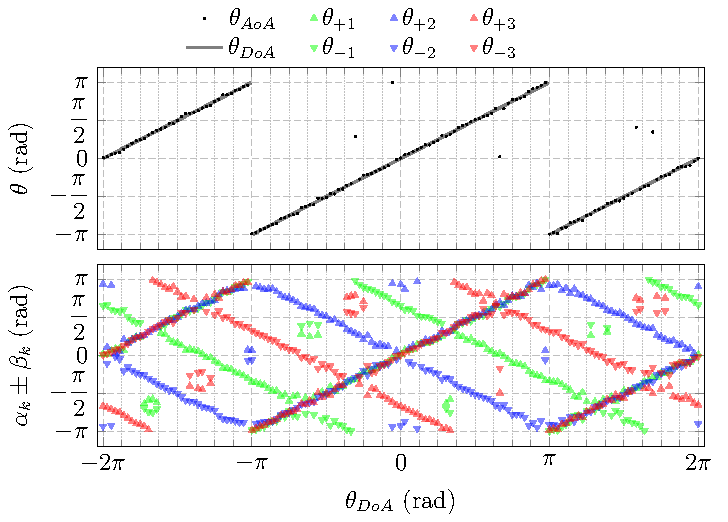
\includegraphics[height=0.785\textheight]{../pictures/simul_POLY_3_R_50_SNR_1_ATT.pdf}
			\caption*{\tiny Fonte: Autor, saída gráfica disponível em \href{https://github.com/HeckRodSav/TG/blob/main/documentation/pictures/POLY_3/simul_POLY_3_R_50_SNR_1_ATT.gif}{\underline{GitHub}}.}
		\end{figure}
	\end{frame}

\subsection{Cinco antenas}
	\begin{frame}{R\textsuperscript{2} para cinco antenas}
		\begin{table}
			\centering
			\begin{tabular}{@{}
				S[table-format = 3.1]
				S[table-format = 3.2, table-model-setup = \bfseries]
				S[table-format = 3.2, table-model-setup = \bfseries]
				@{}}
				\toprule
				{SNR (\unit{\deci\bel})} & {R\textsuperscript{2} sem ATT (\unit{\percent})} & {R\textsuperscript{2} com ATT (\unit{\percent})}
				\\\midrule
				\infinity & \bfseries 100.00 & 100.00\\
				20 & 100.00 & 100.00\\
				17 & 91.90 & 91.89\\
				14 & 91.91 & 91.90\\
				7 & 84.27 & 91.93\\
				0 & \bfseries 80.73 & \bfseries 96.28\\
				\bottomrule
			\end{tabular}
			\caption*{\tiny Fonte: Autor, saídas das simulações disponíveis em \href{https://github.com/HeckRodSav/TG/tree/main/documentation/data/POLY_5}{\underline{GitHub}}.}
		\end{table}
	\end{frame}

	\begin{frame}
		\begin{figure}
			\centering
			\caption*{Caso ideal ($\text{SNR} \rightarrow \qty{\infinity}{\deci\bel}$).}
			% \begin{tikzpicture}
    % \pgfsetfillopacity{0.5}

    \def\fileName{simul_POLY_5_R_50}
    \def\fileAddress{../../code/simul/Output/POLY_5/\fileName.dat}
    % \def\fileAddress{../data/\fileName.dat}

    \def\height{.225\linewidth}
    \def\width{0.75\linewidth}
    \def\distance{0.25cm}
    \def\xmin{-1}
    \def\xmax{101}

    \begin{axis} %configuração do eixo Y esquerdo e eixo X
    [
        name=plot1,
        reverse legend, % inverte a ordem que os items aparecem na legenda
    	% legend style={
        % 	at=(current bounding box.north),
        % 	anchor=south,
        % 	legend columns=6,
        % 	transpose legend,
        % 	draw=none,
        % 	/tikz/every even column/.append style={column sep=0.5cm}
    	% }, % onde exibir
        % axis x line=center,
        % axis y line=center,
        height=\height, % altura da região do gráfico
        width=\width, % largura da região do gráfico
        scale only axis, %
        minor grid style={densely dotted}, % estilo da grade secundária
        major grid style={densely dashed}, % estilo da grade principal
        grid style={lightgray, thin}, % cor das grades
        % axis on top, % forçar grade para ficar por cima do gráfico
        %
        %
        % axis y line*=left, % define gráfico para usar eixo esquerdo sem exibir direito
        y tick label style={
            /pgf/number format/.cd,
            fixed,
            % fixed zerofill,
            precision=1, % quantidade de casas depois da virgula
            /tikz/.cd
        },
        % y filter/.expression={y==0 ? NaN : y},
        scaled y ticks = false,
        ylabel={$\alpha_{k}\pm \beta_{k}$ (\si{\radian})}, % titulo eixo vertical
        % yticklabel={\pgfmathparse{\tick-50}\pgfmathprintnumber{\pgfmathresult}}, % fator multiplicativo para valores do eixo
        y tick label style={/pgf/number format/1000 sep=}, % Altera marcação de milhar
        % yticklabel style={rotate=90},
		ytick={-3.1415, -1.5708, 0, 1.5708, 3.1415},
		yticklabels={$-\pi$,$-\dfrac{\pi}{2}$,$0$,$\dfrac{\pi}{2}$,$\pi$},
        % ytick={0,1,2,3,4,5}, % lista de valores a serem utilizados no eixo
        % ymin=-1,  ymax=4,  % intervalo de valores no eixo y -> na dúvida, deixe comentado
        %
        ymajorgrids=true, % exibir grade principal y
        yminorgrids=true, % exibir grade secundária y
        minor y tick num=4, % contagem de linhas na grade secundária y
        % ybar,
        %
        %
        xlabel={$\theta_{DoA}$ (\si{\radian})}, % título eixo horizontal
        % xticklabel={\pgfmathparse{\tick-50}\pgfmathprintnumber{\pgfmathresult}}, % fator multiplicativo para valores do eixo
        % xticklabels={}, % fator multiplicativo para valores do eixo
		% xtick={0, 12.5, 25, 37.5, 50, 62.6, 75, 87.5, 100},
		% xticklabels={$-2~\pi$,$-\dfrac{3~\pi}{2}$,$-\pi$,$-\dfrac{\pi}{2}$,$0$,$-\dfrac{\pi}{2}$,$\pi$,$-\dfrac{3~\pi}{2}$,$2~\pi$},
		xtick={0, 25, 50, 75, 100},
		xticklabels={$-2 \pi$,$-\pi$,$0$,$\pi$,$2 \pi$},
        % xmode=log,
        % log ticks with fixed point,
        % x filter/.code=\pgfmathparse{#1 + 6.90775527898214},
        x tick label style={
            /pgf/number format/.cd,
            fixed,
            % fixed zerofill,
            precision=1,
            /tikz/.cd,
            /pgf/number format/use comma
        },
        xmin=\xmin, xmax=\xmax, % intervalo de valores no eixo x -> na dúvida, deixe comentado
        scaled x ticks = false,
        %
        xmajorgrids=true, % exibir grade principal x
        xminorgrids=true, % exibir grade secundária x
        minor x tick num=7, % contagem de linhas na grade secundária x
        %
        %
        %
        % unbounded coords=jump,
        % jump threshold/.initial=0.25
    ]

	\addplot[
        cmyk_G,
        mark=triangle*,
		opacity=0.5,
        only marks,
        % smooth
    ] table [
        % col sep=comma,
        x=percent, % cabeçalho da coluna de dados X no arquivo
        y=delta_1_x_5, % cabeçalho da coluna de dados Y no arquivo
    ]
    {\fileAddress};	\label{\fileName.1.1}

    \addplot[
        cmyk_G,
        mark=triangle*,
		opacity=0.5,
		mark options={rotate=180},
        only marks,
        % smooth
    ] table [
        % col sep=comma,
        x=percent, % cabeçalho da coluna de dados X no arquivo
        y=delta_5_x_1, % cabeçalho da coluna de dados Y no arquivo
    ]
    {\fileAddress};	\label{\fileName.1.2}

	\addplot[
        cmyk_B,
        mark=triangle*,
		opacity=0.5,
        only marks,
        % smooth
    ] table [
        % col sep=comma,
        x=percent, % cabeçalho da coluna de dados X no arquivo
        y=delta_2_x_1, % cabeçalho da coluna de dados Y no arquivo
    ]
    {\fileAddress};	\label{\fileName.1.3}

    \addplot[
        cmyk_B,
        mark=triangle*,
		opacity=0.5,
		mark options={rotate=180},
        only marks,
        % smooth
    ] table [
        % col sep=comma,
        x=percent, % cabeçalho da coluna de dados X no arquivo
        y=delta_1_x_2, % cabeçalho da coluna de dados Y no arquivo
    ]
    {\fileAddress};	\label{\fileName.1.4}

	\addplot[
        cmyk_R,
        mark=triangle*,
		opacity=0.5,
        only marks,
        % smooth
    ] table [
        % col sep=comma,
        x=percent, % cabeçalho da coluna de dados X no arquivo
        y=delta_3_x_2, % cabeçalho da coluna de dados Y no arquivo
    ]
    {\fileAddress};	\label{\fileName.1.5}

    \addplot[
        cmyk_R,
        mark=triangle*,
		opacity=0.5,
		mark options={rotate=180},
        only marks,
        % smooth
    ] table [
        % col sep=comma,
        x=percent, % cabeçalho da coluna de dados X no arquivo
        y=delta_2_x_3, % cabeçalho da coluna de dados Y no arquivo
    ]
    {\fileAddress};	\label{\fileName.1.6}

	\addplot[
        cmyk_C,
        mark=triangle*,
		opacity=0.5,
        only marks,
        % smooth
    ] table [
        % col sep=comma,
        x=percent, % cabeçalho da coluna de dados X no arquivo
        y=delta_4_x_3, % cabeçalho da coluna de dados Y no arquivo
    ]
    {\fileAddress};	\label{\fileName.1.7}

    \addplot[
        cmyk_C,
        mark=triangle*,
		opacity=0.5,
		mark options={rotate=180},
        only marks,
        % smooth
    ] table [
        % col sep=comma,
        x=percent, % cabeçalho da coluna de dados X no arquivo
        y=delta_3_x_4, % cabeçalho da coluna de dados Y no arquivo
    ]
    {\fileAddress};	\label{\fileName.1.8}

	\addplot[
        Goldenrod,
        mark=triangle*,
		opacity=0.5,
        only marks,
        % smooth
    ] table [
        % col sep=comma,
        x=percent, % cabeçalho da coluna de dados X no arquivo
        y=delta_5_x_4, % cabeçalho da coluna de dados Y no arquivo
    ]
    {\fileAddress};	\label{\fileName.1.9}

    \addplot[
        Goldenrod,
        mark=triangle*,
		opacity=0.5,
		mark options={rotate=180},
        only marks,
        % smooth
    ] table [
        % col sep=comma,
        x=percent, % cabeçalho da coluna de dados X no arquivo
        y=delta_4_x_5, % cabeçalho da coluna de dados Y no arquivo
    ]
    {\fileAddress};	\label{\fileName.1.10}

    \end{axis}

    % \begin{axis} %configuração do eixo Y direito e legenda
    % [
    %     legend cell align=left, % alinhamento de texto na legenda
    %     % legend pos={outer north east}, % onde exibir caixa de legenda
    %     % reverse legend, % inverte a ordem que os items aparecem na legenda
    % 	legend style={
    %     	at=(current bounding box.north),
    %     	anchor=south,
    %     	legend columns=2,
    %     % 	transpose legend,
    %     	draw=none
    % 	}, % onde exibir
    %     % axis x line=center,
    %     % axis y line=center,
    %     height=\height, % altura da região do gráfico
    %     width=\width, % largura da região do gráfico
    %     scale only axis, %
    %     minor grid style={densely dotted}, % estilo da grade secundária
    %     major grid style={densely dashed}, % estilo da grade principal
    %     grid style={lightgray, thin}, % cor das grades
    %     % axis on top, % forçar grade para ficar por cima do gráfico
    %     %
    %     %
    %     axis y line*=right, % define gráfico para usar eixo direito sem exibir esquerdo
    %     ylabel={$V_{out}$ (\si{\milli\volt})}, % titulo eixo vertical
    %     y tick label style={
    %         /pgf/number format/.cd,
    %         fixed,
    %         % fixed zerofill,
    %         precision=3, % quantidade de casas depois da virgula
    %         /tikz/.cd,
    %         /pgf/number format/use comma
    %     },
    %     % y filter/.expression={y==0 ? NaN : y},
    %     scaled y ticks = false,
    %     % yticklabel={\pgfmathparse{\tick*10^3}\pgfmathprintnumber{\pgfmathresult}}, % fator multiplicativo para valores do eixo
    %     y tick label style={/pgf/number format/1000 sep=}, % Altera marcação de milhar
    %     % yticklabel style={rotate=90},
    %     % ytick={-12,-6,0,6,12}, % lista de valores a serem utilizados no eixo
    %     % ymin=0.76503, ymax=0.76509,  % intervalo de valores no eixo y -> na dúvida, deixe comentado
    %     %
    %     ymajorgrids=false, % exibir grade principal y
    %     yminorgrids=false, % exibir grade secundária y
    %     minor y tick num=4, % contagem de linhas na grade secundária y
    %     % ybar,
    %     %
    %     %
    %     axis x line=none, %oculta eixo inferior quando o gráfico anterior já exibe
    %     % xlabel={Frequência (\si{\hertz})}, % título eixo horizontal
    %     % xticklabel={\pgfmathparse{\tick*10^3}\pgfmathprintnumber{\pgfmathresult}}, % fator multiplicativo para valores do eixo
    %     % xmode=log,
    %     % log ticks with fixed point,
    %     % x filter/.code=\pgfmathparse{#1 + 6.90775527898214},
    %     % x tick label style={
    %     %     /pgf/number format/.cd,
    %     %     fixed,
    %     %     % fixed zerofill,
    %     %     precision=0,
    %     %     /tikz/.cd,
    %     %     /pgf/number format/use comma
    %     % },
    %     xmin=\xmin, xmax=\xmax, % intervalo de valores no eixo x -> na dúvida, deixe comentado
    %     % scaled x ticks = true,
    %     %
    %     % xmajorgrids=true, % exibir grade principal x
    %     % xminorgrids=true, % exibir grade secundária x
    %     % minor x tick num=7, % contagem de linhas na grade secundária x
    %     %
    %     %
    %     %
    % ]



    % \addplot[mark=none,red, thick]
    % table [
    %     x=time, % cabeçalho da coluna de dados X no arquivo
    %     y=vout % cabeçalho da coluna de dados Y no arquivo
    % ]
    % {graficos/dados/booster.dat};  \label{\fileName.1.2}

    % % \addlegendimage{/pgfplots/refstyle=_1_2}

    % % \addplot[ForestGreen, densely dashdotted, thick]
    % % coordinates
    % % {
    % %     (\pgfkeysvalueof{/pgfplots/xmin},12)
    % %     (\pgfkeysvalueof{/pgfplots/xmax},12)
    % % };
    % % % \addlegendentry{$V_{out}=\pm\SI{12}{\volt}$}

    % % \addplot[ForestGreen, densely dashdotted, thick]
    % % coordinates
    % % {
    % %     (\pgfkeysvalueof{/pgfplots/xmin},-12)
    % %     (\pgfkeysvalueof{/pgfplots/xmax},-12)
    % % };

    % \end{axis}

    \begin{axis} %configuração do eixo Y esquerdo e eixo X
    [
        at={($(plot1.north)+(0,\distance)$)},
        anchor=south,
        % reverse legend, % inverte a ordem que os items aparecem na legenda
		legend style={
        	at=(current bounding box.north),
        	anchor=south,
        	legend columns=2,
        	transpose legend,
        	draw=none,
        	/tikz/every even column/.append style={column sep=0.5cm}
    	}, % onde exibir
        samples=505,
        domain=0:100,
        % axis x line=center,
        % axis y line=center,
        height=\height, % altura da região do gráfico
        width=\width, % largura da região do gráfico
        scale only axis, %
        minor grid style={densely dotted}, % estilo da grade secundária
        major grid style={densely dashed}, % estilo da grade principal
        grid style={lightgray, thin}, % cor das grades
        % axis on top, % forçar grade para ficar por cima do gráfico
        %
        %
        % axis y line*=left, % define gráfico para usar eixo esquerdo sem exibir direito
        y tick label style={
            /pgf/number format/.cd,
            fixed,
            % fixed zerofill,
            precision=1, % quantidade de casas depois da virgula
            /tikz/.cd
        },
        % y filter/.expression={y==0 ? NaN : y},
        scaled y ticks = false,
        ylabel={$\theta$ (\si{\radian})}, % titulo eixo vertical
        % yticklabel={\pgfmathparse{\tick*10^3}\pgfmathprintnumber{\pgfmathresult}}, % fator multiplicativo para valores do eixo
        y tick label style={/pgf/number format/1000 sep=}, % Altera marcação de milhar
        % yticklabel style={rotate=90},
		ytick={-3.1415, -1.5708, 0, 1.5708, 3.1415},
		yticklabels={$-\pi$,$-\dfrac{\pi}{2}$,$0$,$\dfrac{\pi}{2}$,$\pi$},
        % ytick={0,1,2,3,4,5}, % lista de valores a serem utilizados no eixo
        % ymin=-1,  ymax=4,  % intervalo de valores no eixo y -> na dúvida, deixe comentado
        %
        ymajorgrids=true, % exibir grade principal y
        yminorgrids=true, % exibir grade secundária y
        minor y tick num=4, % contagem de linhas na grade secundária y
        % ybar,
        %
        %
        % xlabel={Tempo (\si{\milli\second})}, % título eixo horizontal
        % xticklabel={\pgfmathparse{\tick*10^3}\pgfmathprintnumber{\pgfmathresult}}, % fator multiplicativo para valores do eixo
		xtick={0, 25, 50, 75, 100},
        xticklabels={}, % fator multiplicativo para valores do eixo
        % xmode=log,
        % log ticks with fixed point,
        % x filter/.code=\pgfmathparse{#1 + 6.90775527898214},
        x tick label style={
            /pgf/number format/.cd,
            fixed,
            % fixed zerofill,
            precision=1,
            /tikz/.cd,
            /pgf/number format/use comma
        },
        xmin=\xmin, xmax=\xmax, % intervalo de valores no eixo x -> na dúvida, deixe comentado
        scaled x ticks = false,
        %
        xmajorgrids=true, % exibir grade principal x
        xminorgrids=true, % exibir grade secundária x
        minor x tick num=7, % contagem de linhas na grade secundária x
        %
        %
        %
        unbounded coords=jump,
		jump threshold/.initial=0.01
    ]


    \addplot[
        Black,
        mark=*,
		mark size=0.5pt,
        only marks,
        % smooth
    ] table [
        % col sep=comma,
        x=percent, % cabeçalho da coluna de dados X no arquivo
        y=choose_angle, % cabeçalho da coluna de dados Y no arquivo
	]
	{\fileAddress};	\addlegendentry{$\theta_{AoA}$}

	% \addplot[
	% 	Black,
	% 	mark=o,
	% 	mark size=1.5pt,
	% 	only marks,
	% 	opacity=0.5,
    %     thick,
	% 	% smooth
	% ] table [
	% 	% col sep=comma,
	% 	x=percent, % cabeçalho da coluna de dados X no arquivo
	% 	y=ang_W, % cabeçalho da coluna de dados Y no arquivo
	% ]
	% {\fileAddress};
    \addplot [
        Black,
        opacity=0.5,
        mark=none,
        mark size=5pt,
        very thick,
        % only marks,
        % smooth
    ] {((x==25)||(x==75)?nan:pi*(mod(x+25,50)-25)/25)};
    \addlegendentry{$\theta_{DoA}$}


	\addlegendimage{/pgfplots/refstyle=\fileName.1.1}\addlegendentry{$\theta_{+1}$}
	\addlegendimage{/pgfplots/refstyle=\fileName.1.2}\addlegendentry{$\theta_{-1}$}

	\addlegendimage{/pgfplots/refstyle=\fileName.1.3}\addlegendentry{$\theta_{+2}$}
	\addlegendimage{/pgfplots/refstyle=\fileName.1.4}\addlegendentry{$\theta_{-2}$}

    \addlegendimage{/pgfplots/refstyle=\fileName.1.5}\addlegendentry{$\theta_{+3}$}
	\addlegendimage{/pgfplots/refstyle=\fileName.1.6}\addlegendentry{$\theta_{-3}$}

    \addlegendimage{/pgfplots/refstyle=\fileName.1.7}\addlegendentry{$\theta_{+4}$}
	\addlegendimage{/pgfplots/refstyle=\fileName.1.8}\addlegendentry{$\theta_{-4}$}

    \addlegendimage{/pgfplots/refstyle=\fileName.1.9}\addlegendentry{$\theta_{+5}$}
	\addlegendimage{/pgfplots/refstyle=\fileName.1.10}\addlegendentry{$\theta_{-5}$}


    \end{axis}

    % \begin{axis} %configuração do eixo Y direito e legenda
    % [
    %     at={($(plot1.north)+(0,\distance)$)},
    %     anchor=south,
    %     legend cell align=left, % alinhamento de texto na legenda
    %     % legend pos={outer north east}, % onde exibir caixa de legenda
    %     % reverse legend, % inverte a ordem que os items aparecem na legenda
    % 	legend style={
    %     	at=(current bounding box.north),
    %     	anchor=south,
    %     	legend columns=3,
    %     % 	transpose legend,
    %     	draw=none,
    %     	/tikz/every even column/.append style={column sep=0.5cm}
    % 	}, % onde exibir
    %     % axis x line=center,
    %     % axis y line=center,
    %     height=\height, % altura da região do gráfico
    %     width=\width, % largura da região do gráfico
    %     scale only axis, %
    %     minor grid style={densely dotted}, % estilo da grade secundária
    %     major grid style={densely dashed}, % estilo da grade principal
    %     grid style={lightgray, thin}, % cor das grades
    %     % axis on top, % forçar grade para ficar por cima do gráfico
    %     %
    %     %
    %     axis y line*=right, % define gráfico para usar eixo direito sem exibir esquerdo
    %     ylabel={$V_{out}$ (\si{\volt})}, % titulo eixo vertical
    %     y tick label style={
    %         /pgf/number format/.cd,
    %         fixed,
    %         % fixed zerofill,
    %         precision=3, % quantidade de casas depois da virgula
    %         /tikz/.cd,
    %         /pgf/number format/use comma
    %     },
    %     % y filter/.expression={y==0 ? NaN : y},
    %     scaled y ticks = false,
    %     % yticklabel={\pgfmathparse{\tick*10^3}\pgfmathprintnumber{\pgfmathresult}}, % fator multiplicativo para valores do eixo
    %     y tick label style={/pgf/number format/1000 sep=}, % Altera marcação de milhar
    %     % yticklabel style={rotate=90},
    %     % ytick={-12,-6,0,6,12}, % lista de valores a serem utilizados no eixo
    %     % ymin=0.76503, ymax=0.76509,  % intervalo de valores no eixo y -> na dúvida, deixe comentado
    %     %
    %     ymajorgrids=false, % exibir grade principal y
    %     yminorgrids=false, % exibir grade secundária y
    %     minor y tick num=4, % contagem de linhas na grade secundária y
    %     % ybar,
    %     %
    %     %
    %     axis x line=none, %oculta eixo inferior quando o gráfico anterior já exibe
    %     % xlabel={Frequência (\si{\hertz})}, % título eixo horizontal
    %     % xticklabel={\pgfmathparse{\tick*10^3}\pgfmathprintnumber{\pgfmathresult}}, % fator multiplicativo para valores do eixo
    %     % xmode=log,
    %     % log ticks with fixed point,
    %     % x filter/.code=\pgfmathparse{#1 + 6.90775527898214},
    %     % x tick label style={
    %     %     /pgf/number format/.cd,
    %     %     fixed,
    %     %     % fixed zerofill,
    %     %     precision=0,
    %     %     /tikz/.cd,
    %     %     /pgf/number format/use comma
    %     % },
    %     xmin=\xmin, xmax=\xmax, % intervalo de valores no eixo x -> na dúvida, deixe comentado
    %     % scaled x ticks = true,
    %     %
    %     % xmajorgrids=true, % exibir grade principal x
    %     % xminorgrids=true, % exibir grade secundária x
    %     % minor x tick num=10, % contagem de linhas na grade secundária x
    %     %
    %     %
    %     %
    % ]


    % \addlegendimage{/pgfplots/refstyle=_2_1}\addlegendentry{$V_{in}$}
    % \addlegendimage{/pgfplots/refstyle=_2_2}\addlegendentry{$V_{in}$}
    % % \addplot[mark=none,red, thick]
    % % table [
    % %     x=time, % cabeçalho da coluna de dados X no arquivo
    % %     y=vout % cabeçalho da coluna de dados Y no arquivo
    % % ]
    % % {graficos/dados/booster.dat}; % \label{\fileName.1.2}
    % % \addlegendentry{$V_{out}$}

    % \addlegendimage{/pgfplots/refstyle=_1_1}\addlegendentry{$I_{out}$}
    % \addlegendimage{/pgfplots/refstyle=_1_2}\addlegendentry{$I_{out}$}

    % % \addlegendimage{/pgfplots/refstyle=_1_2}

    % % \addplot[ForestGreen, densely dashdotted, thick]
    % % coordinates
    % % {
    % %     (\pgfkeysvalueof{/pgfplots/xmin},12)
    % %     (\pgfkeysvalueof{/pgfplots/xmax},12)
    % % };
    % % % \addlegendentry{$V_{out}=\pm\SI{12}{\volt}$}

    % % \addplot[ForestGreen, densely dashdotted, thick]
    % % coordinates
    % % {
    % %     (\pgfkeysvalueof{/pgfplots/xmin},-12)
    % %     (\pgfkeysvalueof{/pgfplots/xmax},-12)
    % % };

    % \end{axis}



\end{tikzpicture}

			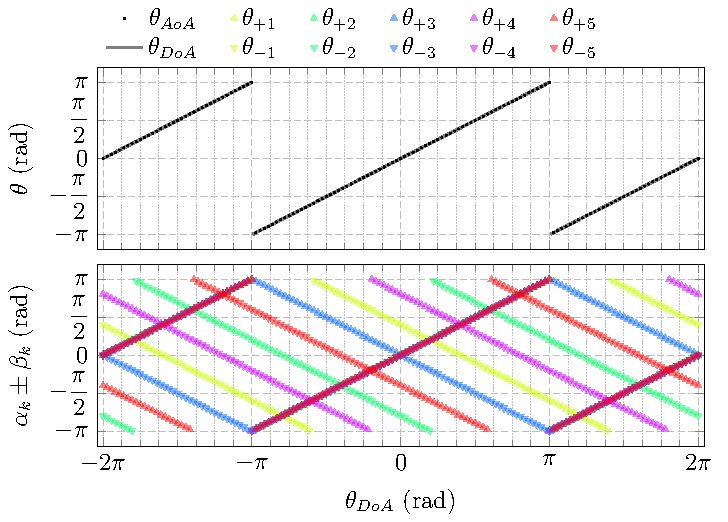
\includegraphics[height=0.785\textheight]{../pictures/simul_POLY_5_R_50.pdf}
			\caption*{\tiny Fonte: Autor, saída gráfica disponível em \href{https://github.com/HeckRodSav/TG/blob/main/documentation/pictures/POLY_5/simul_POLY_5_R_50.gif}{\underline{GitHub}}.}
		\end{figure}
	\end{frame}
	\begin{frame}
		\begin{figure}
			\centering
			\caption*{Caso $\text{SNR} = \SI{0}{\deci\bel}$, sem atenuação.}
			% \begin{tikzpicture}
    % \pgfsetfillopacity{0.5}

    \def\fileName{simul_POLY_5_R_50_SNR_1}
    \def\fileAddress{../../code/simul/Output/POLY_5/\fileName.dat}
    % \def\fileAddress{../data/\fileName.dat}

    \def\height{.225\linewidth}
    \def\width{0.75\linewidth}
    \def\distance{0.25cm}
    \def\xmin{-1}
    \def\xmax{101}

    \begin{axis} %configuração do eixo Y esquerdo e eixo X
    [
        name=plot1,
        reverse legend, % inverte a ordem que os items aparecem na legenda
    	% legend style={
        % 	at=(current bounding box.north),
        % 	anchor=south,
        % 	legend columns=6,
        % 	transpose legend,
        % 	draw=none,
        % 	/tikz/every even column/.append style={column sep=0.5cm}
    	% }, % onde exibir
        % axis x line=center,
        % axis y line=center,
        height=\height, % altura da região do gráfico
        width=\width, % largura da região do gráfico
        scale only axis, %
        minor grid style={densely dotted}, % estilo da grade secundária
        major grid style={densely dashed}, % estilo da grade principal
        grid style={lightgray, thin}, % cor das grades
        % axis on top, % forçar grade para ficar por cima do gráfico
        %
        %
        % axis y line*=left, % define gráfico para usar eixo esquerdo sem exibir direito
        y tick label style={
            /pgf/number format/.cd,
            fixed,
            % fixed zerofill,
            precision=1, % quantidade de casas depois da virgula
            /tikz/.cd
        },
        % y filter/.expression={y==0 ? NaN : y},
        scaled y ticks = false,
        ylabel={$\alpha_{k}\pm \beta_{k}$ (\si{\radian})}, % titulo eixo vertical
        % yticklabel={\pgfmathparse{\tick-50}\pgfmathprintnumber{\pgfmathresult}}, % fator multiplicativo para valores do eixo
        y tick label style={/pgf/number format/1000 sep=}, % Altera marcação de milhar
        % yticklabel style={rotate=90},
		ytick={-3.1415, -1.5708, 0, 1.5708, 3.1415},
		yticklabels={$-\pi$,$-\dfrac{\pi}{2}$,$0$,$\dfrac{\pi}{2}$,$\pi$},
        % ytick={0,1,2,3,4,5}, % lista de valores a serem utilizados no eixo
        % ymin=-1,  ymax=4,  % intervalo de valores no eixo y -> na dúvida, deixe comentado
        %
        ymajorgrids=true, % exibir grade principal y
        yminorgrids=true, % exibir grade secundária y
        minor y tick num=4, % contagem de linhas na grade secundária y
        % ybar,
        %
        %
        xlabel={$\theta_{DoA}$ (\si{\radian})}, % título eixo horizontal
        % xticklabel={\pgfmathparse{\tick-50}\pgfmathprintnumber{\pgfmathresult}}, % fator multiplicativo para valores do eixo
        % xticklabels={}, % fator multiplicativo para valores do eixo
		% xtick={0, 12.5, 25, 37.5, 50, 62.6, 75, 87.5, 100},
		% xticklabels={$-2~\pi$,$-\dfrac{3~\pi}{2}$,$-\pi$,$-\dfrac{\pi}{2}$,$0$,$-\dfrac{\pi}{2}$,$\pi$,$-\dfrac{3~\pi}{2}$,$2~\pi$},
		xtick={0, 25, 50, 75, 100},
		xticklabels={$-2 \pi$,$-\pi$,$0$,$\pi$,$2 \pi$},
        % xmode=log,
        % log ticks with fixed point,
        % x filter/.code=\pgfmathparse{#1 + 6.90775527898214},
        x tick label style={
            /pgf/number format/.cd,
            fixed,
            % fixed zerofill,
            precision=1,
            /tikz/.cd,
            /pgf/number format/use comma
        },
        xmin=\xmin, xmax=\xmax, % intervalo de valores no eixo x -> na dúvida, deixe comentado
        scaled x ticks = false,
        %
        xmajorgrids=true, % exibir grade principal x
        xminorgrids=true, % exibir grade secundária x
        minor x tick num=7, % contagem de linhas na grade secundária x
        %
        %
        %
        % unbounded coords=jump,
        % jump threshold/.initial=0.25
    ]

	\addplot[
        cmyk_G,
        mark=triangle*,
		opacity=0.5,
        only marks,
        % smooth
    ] table [
        % col sep=comma,
        x=percent, % cabeçalho da coluna de dados X no arquivo
        y=delta_1_x_5, % cabeçalho da coluna de dados Y no arquivo
    ]
    {\fileAddress};	\label{\fileName.1.1}

    \addplot[
        cmyk_G,
        mark=triangle*,
		opacity=0.5,
		mark options={rotate=180},
        only marks,
        % smooth
    ] table [
        % col sep=comma,
        x=percent, % cabeçalho da coluna de dados X no arquivo
        y=delta_5_x_1, % cabeçalho da coluna de dados Y no arquivo
    ]
    {\fileAddress};	\label{\fileName.1.2}

	\addplot[
        cmyk_B,
        mark=triangle*,
		opacity=0.5,
        only marks,
        % smooth
    ] table [
        % col sep=comma,
        x=percent, % cabeçalho da coluna de dados X no arquivo
        y=delta_2_x_1, % cabeçalho da coluna de dados Y no arquivo
    ]
    {\fileAddress};	\label{\fileName.1.3}

    \addplot[
        cmyk_B,
        mark=triangle*,
		opacity=0.5,
		mark options={rotate=180},
        only marks,
        % smooth
    ] table [
        % col sep=comma,
        x=percent, % cabeçalho da coluna de dados X no arquivo
        y=delta_1_x_2, % cabeçalho da coluna de dados Y no arquivo
    ]
    {\fileAddress};	\label{\fileName.1.4}

	\addplot[
        cmyk_R,
        mark=triangle*,
		opacity=0.5,
        only marks,
        % smooth
    ] table [
        % col sep=comma,
        x=percent, % cabeçalho da coluna de dados X no arquivo
        y=delta_3_x_2, % cabeçalho da coluna de dados Y no arquivo
    ]
    {\fileAddress};	\label{\fileName.1.5}

    \addplot[
        cmyk_R,
        mark=triangle*,
		opacity=0.5,
		mark options={rotate=180},
        only marks,
        % smooth
    ] table [
        % col sep=comma,
        x=percent, % cabeçalho da coluna de dados X no arquivo
        y=delta_2_x_3, % cabeçalho da coluna de dados Y no arquivo
    ]
    {\fileAddress};	\label{\fileName.1.6}

	\addplot[
        cmyk_C,
        mark=triangle*,
		opacity=0.5,
        only marks,
        % smooth
    ] table [
        % col sep=comma,
        x=percent, % cabeçalho da coluna de dados X no arquivo
        y=delta_4_x_3, % cabeçalho da coluna de dados Y no arquivo
    ]
    {\fileAddress};	\label{\fileName.1.7}

    \addplot[
        cmyk_C,
        mark=triangle*,
		opacity=0.5,
		mark options={rotate=180},
        only marks,
        % smooth
    ] table [
        % col sep=comma,
        x=percent, % cabeçalho da coluna de dados X no arquivo
        y=delta_3_x_4, % cabeçalho da coluna de dados Y no arquivo
    ]
    {\fileAddress};	\label{\fileName.1.8}

	\addplot[
        Goldenrod,
        mark=triangle*,
		opacity=0.5,
        only marks,
        % smooth
    ] table [
        % col sep=comma,
        x=percent, % cabeçalho da coluna de dados X no arquivo
        y=delta_5_x_4, % cabeçalho da coluna de dados Y no arquivo
    ]
    {\fileAddress};	\label{\fileName.1.9}

    \addplot[
        Goldenrod,
        mark=triangle*,
		opacity=0.5,
		mark options={rotate=180},
        only marks,
        % smooth
    ] table [
        % col sep=comma,
        x=percent, % cabeçalho da coluna de dados X no arquivo
        y=delta_4_x_5, % cabeçalho da coluna de dados Y no arquivo
    ]
    {\fileAddress};	\label{\fileName.1.10}

    \end{axis}

    % \begin{axis} %configuração do eixo Y direito e legenda
    % [
    %     legend cell align=left, % alinhamento de texto na legenda
    %     % legend pos={outer north east}, % onde exibir caixa de legenda
    %     % reverse legend, % inverte a ordem que os items aparecem na legenda
    % 	legend style={
    %     	at=(current bounding box.north),
    %     	anchor=south,
    %     	legend columns=2,
    %     % 	transpose legend,
    %     	draw=none
    % 	}, % onde exibir
    %     % axis x line=center,
    %     % axis y line=center,
    %     height=\height, % altura da região do gráfico
    %     width=\width, % largura da região do gráfico
    %     scale only axis, %
    %     minor grid style={densely dotted}, % estilo da grade secundária
    %     major grid style={densely dashed}, % estilo da grade principal
    %     grid style={lightgray, thin}, % cor das grades
    %     % axis on top, % forçar grade para ficar por cima do gráfico
    %     %
    %     %
    %     axis y line*=right, % define gráfico para usar eixo direito sem exibir esquerdo
    %     ylabel={$V_{out}$ (\si{\milli\volt})}, % titulo eixo vertical
    %     y tick label style={
    %         /pgf/number format/.cd,
    %         fixed,
    %         % fixed zerofill,
    %         precision=3, % quantidade de casas depois da virgula
    %         /tikz/.cd,
    %         /pgf/number format/use comma
    %     },
    %     % y filter/.expression={y==0 ? NaN : y},
    %     scaled y ticks = false,
    %     % yticklabel={\pgfmathparse{\tick*10^3}\pgfmathprintnumber{\pgfmathresult}}, % fator multiplicativo para valores do eixo
    %     y tick label style={/pgf/number format/1000 sep=}, % Altera marcação de milhar
    %     % yticklabel style={rotate=90},
    %     % ytick={-12,-6,0,6,12}, % lista de valores a serem utilizados no eixo
    %     % ymin=0.76503, ymax=0.76509,  % intervalo de valores no eixo y -> na dúvida, deixe comentado
    %     %
    %     ymajorgrids=false, % exibir grade principal y
    %     yminorgrids=false, % exibir grade secundária y
    %     minor y tick num=4, % contagem de linhas na grade secundária y
    %     % ybar,
    %     %
    %     %
    %     axis x line=none, %oculta eixo inferior quando o gráfico anterior já exibe
    %     % xlabel={Frequência (\si{\hertz})}, % título eixo horizontal
    %     % xticklabel={\pgfmathparse{\tick*10^3}\pgfmathprintnumber{\pgfmathresult}}, % fator multiplicativo para valores do eixo
    %     % xmode=log,
    %     % log ticks with fixed point,
    %     % x filter/.code=\pgfmathparse{#1 + 6.90775527898214},
    %     % x tick label style={
    %     %     /pgf/number format/.cd,
    %     %     fixed,
    %     %     % fixed zerofill,
    %     %     precision=0,
    %     %     /tikz/.cd,
    %     %     /pgf/number format/use comma
    %     % },
    %     xmin=\xmin, xmax=\xmax, % intervalo de valores no eixo x -> na dúvida, deixe comentado
    %     % scaled x ticks = true,
    %     %
    %     % xmajorgrids=true, % exibir grade principal x
    %     % xminorgrids=true, % exibir grade secundária x
    %     % minor x tick num=7, % contagem de linhas na grade secundária x
    %     %
    %     %
    %     %
    % ]



    % \addplot[mark=none,red, thick]
    % table [
    %     x=time, % cabeçalho da coluna de dados X no arquivo
    %     y=vout % cabeçalho da coluna de dados Y no arquivo
    % ]
    % {graficos/dados/booster.dat};  \label{\fileName.1.2}

    % % \addlegendimage{/pgfplots/refstyle=_1_2}

    % % \addplot[ForestGreen, densely dashdotted, thick]
    % % coordinates
    % % {
    % %     (\pgfkeysvalueof{/pgfplots/xmin},12)
    % %     (\pgfkeysvalueof{/pgfplots/xmax},12)
    % % };
    % % % \addlegendentry{$V_{out}=\pm\SI{12}{\volt}$}

    % % \addplot[ForestGreen, densely dashdotted, thick]
    % % coordinates
    % % {
    % %     (\pgfkeysvalueof{/pgfplots/xmin},-12)
    % %     (\pgfkeysvalueof{/pgfplots/xmax},-12)
    % % };

    % \end{axis}

    \begin{axis} %configuração do eixo Y esquerdo e eixo X
    [
        at={($(plot1.north)+(0,\distance)$)},
        anchor=south,
        % reverse legend, % inverte a ordem que os items aparecem na legenda
		legend style={
        	at=(current bounding box.north),
        	anchor=south,
        	legend columns=2,
        	transpose legend,
        	draw=none,
        	/tikz/every even column/.append style={column sep=0.5cm}
    	}, % onde exibir
        samples=505,
        domain=0:100,
        % axis x line=center,
        % axis y line=center,
        height=\height, % altura da região do gráfico
        width=\width, % largura da região do gráfico
        scale only axis, %
        minor grid style={densely dotted}, % estilo da grade secundária
        major grid style={densely dashed}, % estilo da grade principal
        grid style={lightgray, thin}, % cor das grades
        % axis on top, % forçar grade para ficar por cima do gráfico
        %
        %
        % axis y line*=left, % define gráfico para usar eixo esquerdo sem exibir direito
        y tick label style={
            /pgf/number format/.cd,
            fixed,
            % fixed zerofill,
            precision=1, % quantidade de casas depois da virgula
            /tikz/.cd
        },
        % y filter/.expression={y==0 ? NaN : y},
        scaled y ticks = false,
        ylabel={$\theta$ (\si{\radian})}, % titulo eixo vertical
        % yticklabel={\pgfmathparse{\tick*10^3}\pgfmathprintnumber{\pgfmathresult}}, % fator multiplicativo para valores do eixo
        y tick label style={/pgf/number format/1000 sep=}, % Altera marcação de milhar
        % yticklabel style={rotate=90},
		ytick={-3.1415, -1.5708, 0, 1.5708, 3.1415},
		yticklabels={$-\pi$,$-\dfrac{\pi}{2}$,$0$,$\dfrac{\pi}{2}$,$\pi$},
        % ytick={0,1,2,3,4,5}, % lista de valores a serem utilizados no eixo
        % ymin=-1,  ymax=4,  % intervalo de valores no eixo y -> na dúvida, deixe comentado
        %
        ymajorgrids=true, % exibir grade principal y
        yminorgrids=true, % exibir grade secundária y
        minor y tick num=4, % contagem de linhas na grade secundária y
        % ybar,
        %
        %
        % xlabel={Tempo (\si{\milli\second})}, % título eixo horizontal
        % xticklabel={\pgfmathparse{\tick*10^3}\pgfmathprintnumber{\pgfmathresult}}, % fator multiplicativo para valores do eixo
		xtick={0, 25, 50, 75, 100},
        xticklabels={}, % fator multiplicativo para valores do eixo
        % xmode=log,
        % log ticks with fixed point,
        % x filter/.code=\pgfmathparse{#1 + 6.90775527898214},
        x tick label style={
            /pgf/number format/.cd,
            fixed,
            % fixed zerofill,
            precision=1,
            /tikz/.cd,
            /pgf/number format/use comma
        },
        xmin=\xmin, xmax=\xmax, % intervalo de valores no eixo x -> na dúvida, deixe comentado
        scaled x ticks = false,
        %
        xmajorgrids=true, % exibir grade principal x
        xminorgrids=true, % exibir grade secundária x
        minor x tick num=7, % contagem de linhas na grade secundária x
        %
        %
        %
        unbounded coords=jump,
		jump threshold/.initial=0.01
    ]


    \addplot[
        Black,
        mark=*,
		mark size=0.5pt,
        only marks,
        % smooth
    ] table [
        % col sep=comma,
        x=percent, % cabeçalho da coluna de dados X no arquivo
        y=choose_angle, % cabeçalho da coluna de dados Y no arquivo
	]
	{\fileAddress};	\addlegendentry{$\theta_{AoA}$}

	% \addplot[
	% 	Black,
	% 	mark=o,
	% 	mark size=1.5pt,
	% 	only marks,
	% 	opacity=0.5,
    %     thick,
	% 	% smooth
	% ] table [
	% 	% col sep=comma,
	% 	x=percent, % cabeçalho da coluna de dados X no arquivo
	% 	y=ang_W, % cabeçalho da coluna de dados Y no arquivo
	% ]
	% {\fileAddress};
    \addplot [
        Black,
        opacity=0.5,
        mark=none,
        mark size=5pt,
        very thick,
        % only marks,
        % smooth
    ] {((x==25)||(x==75)?nan:pi*(mod(x+25,50)-25)/25)};
    \addlegendentry{$\theta_{DoA}$}


	\addlegendimage{/pgfplots/refstyle=\fileName.1.1}\addlegendentry{$\theta_{+1}$}
	\addlegendimage{/pgfplots/refstyle=\fileName.1.2}\addlegendentry{$\theta_{-1}$}

	\addlegendimage{/pgfplots/refstyle=\fileName.1.3}\addlegendentry{$\theta_{+2}$}
	\addlegendimage{/pgfplots/refstyle=\fileName.1.4}\addlegendentry{$\theta_{-2}$}

    \addlegendimage{/pgfplots/refstyle=\fileName.1.5}\addlegendentry{$\theta_{+3}$}
	\addlegendimage{/pgfplots/refstyle=\fileName.1.6}\addlegendentry{$\theta_{-3}$}

    \addlegendimage{/pgfplots/refstyle=\fileName.1.7}\addlegendentry{$\theta_{+4}$}
	\addlegendimage{/pgfplots/refstyle=\fileName.1.8}\addlegendentry{$\theta_{-4}$}

    \addlegendimage{/pgfplots/refstyle=\fileName.1.9}\addlegendentry{$\theta_{+5}$}
	\addlegendimage{/pgfplots/refstyle=\fileName.1.10}\addlegendentry{$\theta_{-5}$}


    \end{axis}

    % \begin{axis} %configuração do eixo Y direito e legenda
    % [
    %     at={($(plot1.north)+(0,\distance)$)},
    %     anchor=south,
    %     legend cell align=left, % alinhamento de texto na legenda
    %     % legend pos={outer north east}, % onde exibir caixa de legenda
    %     % reverse legend, % inverte a ordem que os items aparecem na legenda
    % 	legend style={
    %     	at=(current bounding box.north),
    %     	anchor=south,
    %     	legend columns=3,
    %     % 	transpose legend,
    %     	draw=none,
    %     	/tikz/every even column/.append style={column sep=0.5cm}
    % 	}, % onde exibir
    %     % axis x line=center,
    %     % axis y line=center,
    %     height=\height, % altura da região do gráfico
    %     width=\width, % largura da região do gráfico
    %     scale only axis, %
    %     minor grid style={densely dotted}, % estilo da grade secundária
    %     major grid style={densely dashed}, % estilo da grade principal
    %     grid style={lightgray, thin}, % cor das grades
    %     % axis on top, % forçar grade para ficar por cima do gráfico
    %     %
    %     %
    %     axis y line*=right, % define gráfico para usar eixo direito sem exibir esquerdo
    %     ylabel={$V_{out}$ (\si{\volt})}, % titulo eixo vertical
    %     y tick label style={
    %         /pgf/number format/.cd,
    %         fixed,
    %         % fixed zerofill,
    %         precision=3, % quantidade de casas depois da virgula
    %         /tikz/.cd,
    %         /pgf/number format/use comma
    %     },
    %     % y filter/.expression={y==0 ? NaN : y},
    %     scaled y ticks = false,
    %     % yticklabel={\pgfmathparse{\tick*10^3}\pgfmathprintnumber{\pgfmathresult}}, % fator multiplicativo para valores do eixo
    %     y tick label style={/pgf/number format/1000 sep=}, % Altera marcação de milhar
    %     % yticklabel style={rotate=90},
    %     % ytick={-12,-6,0,6,12}, % lista de valores a serem utilizados no eixo
    %     % ymin=0.76503, ymax=0.76509,  % intervalo de valores no eixo y -> na dúvida, deixe comentado
    %     %
    %     ymajorgrids=false, % exibir grade principal y
    %     yminorgrids=false, % exibir grade secundária y
    %     minor y tick num=4, % contagem de linhas na grade secundária y
    %     % ybar,
    %     %
    %     %
    %     axis x line=none, %oculta eixo inferior quando o gráfico anterior já exibe
    %     % xlabel={Frequência (\si{\hertz})}, % título eixo horizontal
    %     % xticklabel={\pgfmathparse{\tick*10^3}\pgfmathprintnumber{\pgfmathresult}}, % fator multiplicativo para valores do eixo
    %     % xmode=log,
    %     % log ticks with fixed point,
    %     % x filter/.code=\pgfmathparse{#1 + 6.90775527898214},
    %     % x tick label style={
    %     %     /pgf/number format/.cd,
    %     %     fixed,
    %     %     % fixed zerofill,
    %     %     precision=0,
    %     %     /tikz/.cd,
    %     %     /pgf/number format/use comma
    %     % },
    %     xmin=\xmin, xmax=\xmax, % intervalo de valores no eixo x -> na dúvida, deixe comentado
    %     % scaled x ticks = true,
    %     %
    %     % xmajorgrids=true, % exibir grade principal x
    %     % xminorgrids=true, % exibir grade secundária x
    %     % minor x tick num=10, % contagem de linhas na grade secundária x
    %     %
    %     %
    %     %
    % ]


    % \addlegendimage{/pgfplots/refstyle=_2_1}\addlegendentry{$V_{in}$}
    % \addlegendimage{/pgfplots/refstyle=_2_2}\addlegendentry{$V_{in}$}
    % % \addplot[mark=none,red, thick]
    % % table [
    % %     x=time, % cabeçalho da coluna de dados X no arquivo
    % %     y=vout % cabeçalho da coluna de dados Y no arquivo
    % % ]
    % % {graficos/dados/booster.dat}; % \label{\fileName.1.2}
    % % \addlegendentry{$V_{out}$}

    % \addlegendimage{/pgfplots/refstyle=_1_1}\addlegendentry{$I_{out}$}
    % \addlegendimage{/pgfplots/refstyle=_1_2}\addlegendentry{$I_{out}$}

    % % \addlegendimage{/pgfplots/refstyle=_1_2}

    % % \addplot[ForestGreen, densely dashdotted, thick]
    % % coordinates
    % % {
    % %     (\pgfkeysvalueof{/pgfplots/xmin},12)
    % %     (\pgfkeysvalueof{/pgfplots/xmax},12)
    % % };
    % % % \addlegendentry{$V_{out}=\pm\SI{12}{\volt}$}

    % % \addplot[ForestGreen, densely dashdotted, thick]
    % % coordinates
    % % {
    % %     (\pgfkeysvalueof{/pgfplots/xmin},-12)
    % %     (\pgfkeysvalueof{/pgfplots/xmax},-12)
    % % };

    % \end{axis}



\end{tikzpicture}

			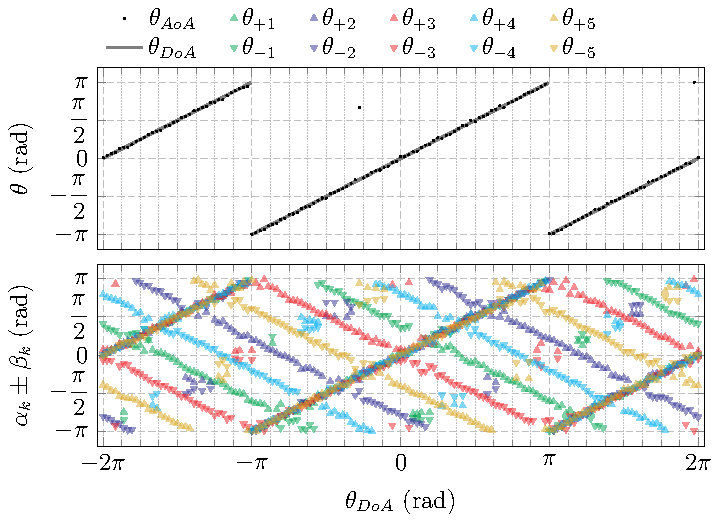
\includegraphics[height=0.785\textheight]{../pictures/simul_POLY_5_R_50_SNR_1.pdf}
			\caption*{\tiny Fonte: Autor, saída gráfica disponível em \href{https://github.com/HeckRodSav/TG/blob/main/documentation/pictures/POLY_5/simul_POLY_5_R_50_SNR_1.gif}{\underline{GitHub}}.}
		\end{figure}
	\end{frame}
	\begin{frame}
		\begin{figure}
			\centering
			\caption*{Caso $\text{SNR} = \SI{0}{\deci\bel}$, com atenuação.}
			% \begin{tikzpicture}
    % \pgfsetfillopacity{0.5}

    \def\fileName{simul_POLY_5_R_50_SNR_1_ATT}
    % \def\fileAddress{../../code/simul/Output/POLY_5/\fileName.dat}
    \def\fileAddress{../data/POLY_5/\fileName.dat}
    % \def\fileAddress{../data/\fileName.dat}

    \def\height{.225\linewidth}
    \def\width{0.75\linewidth}
    \def\distance{0.25cm}
    \def\xmin{-1}
    \def\xmax{101}

    \begin{axis} %configuração do eixo Y esquerdo e eixo X
    [
        name=plot1,
        reverse legend, % inverte a ordem que os items aparecem na legenda
    	% legend style={
        % 	at=(current bounding box.north),
        % 	anchor=south,
        % 	legend columns=6,
        % 	transpose legend,
        % 	draw=none,
        % 	/tikz/every even column/.append style={column sep=0.5cm}
    	% }, % onde exibir
        % axis x line=center,
        % axis y line=center,
        height=\height, % altura da região do gráfico
        width=\width, % largura da região do gráfico
        scale only axis, %
        minor grid style={densely dotted}, % estilo da grade secundária
        major grid style={densely dashed}, % estilo da grade principal
        grid style={lightgray, thin}, % cor das grades
        % axis on top, % forçar grade para ficar por cima do gráfico
        %
        %
        % axis y line*=left, % define gráfico para usar eixo esquerdo sem exibir direito
        y tick label style={
            /pgf/number format/.cd,
            fixed,
            % fixed zerofill,
            precision=1, % quantidade de casas depois da virgula
            /tikz/.cd
        },
        % y filter/.expression={y==0 ? NaN : y},
        scaled y ticks = false,
        ylabel={$\alpha_{k}\pm \beta_{k}$ (\si{\radian})}, % titulo eixo vertical
        % yticklabel={\pgfmathparse{\tick-50}\pgfmathprintnumber{\pgfmathresult}}, % fator multiplicativo para valores do eixo
        y tick label style={/pgf/number format/1000 sep=}, % Altera marcação de milhar
        % yticklabel style={rotate=90},
		ytick={-3.1415, -1.5708, 0, 1.5708, 3.1415},
		yticklabels={$-\pi$,$-\dfrac{\pi}{2}$,$0$,$\dfrac{\pi}{2}$,$\pi$},
        % ytick={0,1,2,3,4,5}, % lista de valores a serem utilizados no eixo
        % ymin=-1,  ymax=4,  % intervalo de valores no eixo y -> na dúvida, deixe comentado
        %
        ymajorgrids=true, % exibir grade principal y
        yminorgrids=true, % exibir grade secundária y
        minor y tick num=4, % contagem de linhas na grade secundária y
        % ybar,
        %
        %
        xlabel={$\theta_{DoA}$ (\si{\radian})}, % título eixo horizontal
        % xticklabel={\pgfmathparse{\tick-50}\pgfmathprintnumber{\pgfmathresult}}, % fator multiplicativo para valores do eixo
        % xticklabels={}, % fator multiplicativo para valores do eixo
		% xtick={0, 12.5, 25, 37.5, 50, 62.6, 75, 87.5, 100},
		% xticklabels={$-2~\pi$,$-\dfrac{3~\pi}{2}$,$-\pi$,$-\dfrac{\pi}{2}$,$0$,$-\dfrac{\pi}{2}$,$\pi$,$-\dfrac{3~\pi}{2}$,$2~\pi$},
		xtick={0, 25, 50, 75, 100},
		xticklabels={$-2 \pi$,$-\pi$,$0$,$\pi$,$2 \pi$},
        % xmode=log,
        % log ticks with fixed point,
        % x filter/.code=\pgfmathparse{#1 + 6.90775527898214},
        x tick label style={
            /pgf/number format/.cd,
            fixed,
            % fixed zerofill,
            precision=1,
            /tikz/.cd,
            /pgf/number format/use comma
        },
        xmin=\xmin, xmax=\xmax, % intervalo de valores no eixo x -> na dúvida, deixe comentado
        scaled x ticks = false,
        %
        xmajorgrids=true, % exibir grade principal x
        xminorgrids=true, % exibir grade secundária x
        minor x tick num=7, % contagem de linhas na grade secundária x
        %
        %
        %
        % unbounded coords=jump,
        % jump threshold/.initial=0.25
    ]

	\addplot[
        cmyk_G,
        mark=triangle*,
		opacity=0.5,
        only marks,
        % smooth
    ] table [
        % col sep=comma,
        x=percent, % cabeçalho da coluna de dados X no arquivo
        y=delta_1_x_5, % cabeçalho da coluna de dados Y no arquivo
    ]
    {\fileAddress};	\label{\fileName.1.1}

    \addplot[
        cmyk_G,
        mark=triangle*,
		opacity=0.5,
		mark options={rotate=180},
        only marks,
        % smooth
    ] table [
        % col sep=comma,
        x=percent, % cabeçalho da coluna de dados X no arquivo
        y=delta_5_x_1, % cabeçalho da coluna de dados Y no arquivo
    ]
    {\fileAddress};	\label{\fileName.1.2}

	\addplot[
        cmyk_B,
        mark=triangle*,
		opacity=0.5,
        only marks,
        % smooth
    ] table [
        % col sep=comma,
        x=percent, % cabeçalho da coluna de dados X no arquivo
        y=delta_2_x_1, % cabeçalho da coluna de dados Y no arquivo
    ]
    {\fileAddress};	\label{\fileName.1.3}

    \addplot[
        cmyk_B,
        mark=triangle*,
		opacity=0.5,
		mark options={rotate=180},
        only marks,
        % smooth
    ] table [
        % col sep=comma,
        x=percent, % cabeçalho da coluna de dados X no arquivo
        y=delta_1_x_2, % cabeçalho da coluna de dados Y no arquivo
    ]
    {\fileAddress};	\label{\fileName.1.4}

	\addplot[
        cmyk_R,
        mark=triangle*,
		opacity=0.5,
        only marks,
        % smooth
    ] table [
        % col sep=comma,
        x=percent, % cabeçalho da coluna de dados X no arquivo
        y=delta_3_x_2, % cabeçalho da coluna de dados Y no arquivo
    ]
    {\fileAddress};	\label{\fileName.1.5}

    \addplot[
        cmyk_R,
        mark=triangle*,
		opacity=0.5,
		mark options={rotate=180},
        only marks,
        % smooth
    ] table [
        % col sep=comma,
        x=percent, % cabeçalho da coluna de dados X no arquivo
        y=delta_2_x_3, % cabeçalho da coluna de dados Y no arquivo
    ]
    {\fileAddress};	\label{\fileName.1.6}

	\addplot[
        cmyk_C,
        mark=triangle*,
		opacity=0.5,
        only marks,
        % smooth
    ] table [
        % col sep=comma,
        x=percent, % cabeçalho da coluna de dados X no arquivo
        y=delta_4_x_3, % cabeçalho da coluna de dados Y no arquivo
    ]
    {\fileAddress};	\label{\fileName.1.7}

    \addplot[
        cmyk_C,
        mark=triangle*,
		opacity=0.5,
		mark options={rotate=180},
        only marks,
        % smooth
    ] table [
        % col sep=comma,
        x=percent, % cabeçalho da coluna de dados X no arquivo
        y=delta_3_x_4, % cabeçalho da coluna de dados Y no arquivo
    ]
    {\fileAddress};	\label{\fileName.1.8}

	\addplot[
        Goldenrod,
        mark=triangle*,
		opacity=0.5,
        only marks,
        % smooth
    ] table [
        % col sep=comma,
        x=percent, % cabeçalho da coluna de dados X no arquivo
        y=delta_5_x_4, % cabeçalho da coluna de dados Y no arquivo
    ]
    {\fileAddress};	\label{\fileName.1.9}

    \addplot[
        Goldenrod,
        mark=triangle*,
		opacity=0.5,
		mark options={rotate=180},
        only marks,
        % smooth
    ] table [
        % col sep=comma,
        x=percent, % cabeçalho da coluna de dados X no arquivo
        y=delta_4_x_5, % cabeçalho da coluna de dados Y no arquivo
    ]
    {\fileAddress};	\label{\fileName.1.10}

    \end{axis}

    % \begin{axis} %configuração do eixo Y direito e legenda
    % [
    %     legend cell align=left, % alinhamento de texto na legenda
    %     % legend pos={outer north east}, % onde exibir caixa de legenda
    %     % reverse legend, % inverte a ordem que os items aparecem na legenda
    % 	legend style={
    %     	at=(current bounding box.north),
    %     	anchor=south,
    %     	legend columns=2,
    %     % 	transpose legend,
    %     	draw=none
    % 	}, % onde exibir
    %     % axis x line=center,
    %     % axis y line=center,
    %     height=\height, % altura da região do gráfico
    %     width=\width, % largura da região do gráfico
    %     scale only axis, %
    %     minor grid style={densely dotted}, % estilo da grade secundária
    %     major grid style={densely dashed}, % estilo da grade principal
    %     grid style={lightgray, thin}, % cor das grades
    %     % axis on top, % forçar grade para ficar por cima do gráfico
    %     %
    %     %
    %     axis y line*=right, % define gráfico para usar eixo direito sem exibir esquerdo
    %     ylabel={$V_{out}$ (\si{\milli\volt})}, % titulo eixo vertical
    %     y tick label style={
    %         /pgf/number format/.cd,
    %         fixed,
    %         % fixed zerofill,
    %         precision=3, % quantidade de casas depois da virgula
    %         /tikz/.cd,
    %         /pgf/number format/use comma
    %     },
    %     % y filter/.expression={y==0 ? NaN : y},
    %     scaled y ticks = false,
    %     % yticklabel={\pgfmathparse{\tick*10^3}\pgfmathprintnumber{\pgfmathresult}}, % fator multiplicativo para valores do eixo
    %     y tick label style={/pgf/number format/1000 sep=}, % Altera marcação de milhar
    %     % yticklabel style={rotate=90},
    %     % ytick={-12,-6,0,6,12}, % lista de valores a serem utilizados no eixo
    %     % ymin=0.76503, ymax=0.76509,  % intervalo de valores no eixo y -> na dúvida, deixe comentado
    %     %
    %     ymajorgrids=false, % exibir grade principal y
    %     yminorgrids=false, % exibir grade secundária y
    %     minor y tick num=4, % contagem de linhas na grade secundária y
    %     % ybar,
    %     %
    %     %
    %     axis x line=none, %oculta eixo inferior quando o gráfico anterior já exibe
    %     % xlabel={Frequência (\si{\hertz})}, % título eixo horizontal
    %     % xticklabel={\pgfmathparse{\tick*10^3}\pgfmathprintnumber{\pgfmathresult}}, % fator multiplicativo para valores do eixo
    %     % xmode=log,
    %     % log ticks with fixed point,
    %     % x filter/.code=\pgfmathparse{#1 + 6.90775527898214},
    %     % x tick label style={
    %     %     /pgf/number format/.cd,
    %     %     fixed,
    %     %     % fixed zerofill,
    %     %     precision=0,
    %     %     /tikz/.cd,
    %     %     /pgf/number format/use comma
    %     % },
    %     xmin=\xmin, xmax=\xmax, % intervalo de valores no eixo x -> na dúvida, deixe comentado
    %     % scaled x ticks = true,
    %     %
    %     % xmajorgrids=true, % exibir grade principal x
    %     % xminorgrids=true, % exibir grade secundária x
    %     % minor x tick num=7, % contagem de linhas na grade secundária x
    %     %
    %     %
    %     %
    % ]



    % \addplot[mark=none,red, thick]
    % table [
    %     x=time, % cabeçalho da coluna de dados X no arquivo
    %     y=vout % cabeçalho da coluna de dados Y no arquivo
    % ]
    % {graficos/dados/booster.dat};  \label{\fileName.1.2}

    % % \addlegendimage{/pgfplots/refstyle=_1_2}

    % % \addplot[ForestGreen, densely dashdotted, thick]
    % % coordinates
    % % {
    % %     (\pgfkeysvalueof{/pgfplots/xmin},12)
    % %     (\pgfkeysvalueof{/pgfplots/xmax},12)
    % % };
    % % % \addlegendentry{$V_{out}=\pm\SI{12}{\volt}$}

    % % \addplot[ForestGreen, densely dashdotted, thick]
    % % coordinates
    % % {
    % %     (\pgfkeysvalueof{/pgfplots/xmin},-12)
    % %     (\pgfkeysvalueof{/pgfplots/xmax},-12)
    % % };

    % \end{axis}

    \begin{axis} %configuração do eixo Y esquerdo e eixo X
    [
        at={($(plot1.north)+(0,\distance)$)},
        anchor=south,
        % reverse legend, % inverte a ordem que os items aparecem na legenda
		legend style={
        	at=(current bounding box.north),
        	anchor=south,
        	legend columns=2,
        	transpose legend,
        	draw=none,
        	/tikz/every even column/.append style={column sep=0.5cm}
    	}, % onde exibir
        samples=505,
        domain=0:100,
        % axis x line=center,
        % axis y line=center,
        height=\height, % altura da região do gráfico
        width=\width, % largura da região do gráfico
        scale only axis, %
        minor grid style={densely dotted}, % estilo da grade secundária
        major grid style={densely dashed}, % estilo da grade principal
        grid style={lightgray, thin}, % cor das grades
        % axis on top, % forçar grade para ficar por cima do gráfico
        %
        %
        % axis y line*=left, % define gráfico para usar eixo esquerdo sem exibir direito
        y tick label style={
            /pgf/number format/.cd,
            fixed,
            % fixed zerofill,
            precision=1, % quantidade de casas depois da virgula
            /tikz/.cd
        },
        % y filter/.expression={y==0 ? NaN : y},
        scaled y ticks = false,
        ylabel={$\theta$ (\si{\radian})}, % titulo eixo vertical
        % yticklabel={\pgfmathparse{\tick*10^3}\pgfmathprintnumber{\pgfmathresult}}, % fator multiplicativo para valores do eixo
        y tick label style={/pgf/number format/1000 sep=}, % Altera marcação de milhar
        % yticklabel style={rotate=90},
		ytick={-3.1415, -1.5708, 0, 1.5708, 3.1415},
		yticklabels={$-\pi$,$-\dfrac{\pi}{2}$,$0$,$\dfrac{\pi}{2}$,$\pi$},
        % ytick={0,1,2,3,4,5}, % lista de valores a serem utilizados no eixo
        % ymin=-1,  ymax=4,  % intervalo de valores no eixo y -> na dúvida, deixe comentado
        %
        ymajorgrids=true, % exibir grade principal y
        yminorgrids=true, % exibir grade secundária y
        minor y tick num=4, % contagem de linhas na grade secundária y
        % ybar,
        %
        %
        % xlabel={Tempo (\si{\milli\second})}, % título eixo horizontal
        % xticklabel={\pgfmathparse{\tick*10^3}\pgfmathprintnumber{\pgfmathresult}}, % fator multiplicativo para valores do eixo
		xtick={0, 25, 50, 75, 100},
        xticklabels={}, % fator multiplicativo para valores do eixo
        % xmode=log,
        % log ticks with fixed point,
        % x filter/.code=\pgfmathparse{#1 + 6.90775527898214},
        x tick label style={
            /pgf/number format/.cd,
            fixed,
            % fixed zerofill,
            precision=1,
            /tikz/.cd,
            /pgf/number format/use comma
        },
        xmin=\xmin, xmax=\xmax, % intervalo de valores no eixo x -> na dúvida, deixe comentado
        scaled x ticks = false,
        %
        xmajorgrids=true, % exibir grade principal x
        xminorgrids=true, % exibir grade secundária x
        minor x tick num=7, % contagem de linhas na grade secundária x
        %
        %
        %
        unbounded coords=jump,
		jump threshold/.initial=0.01
    ]


    \addplot[
        Black,
        mark=*,
		mark size=0.5pt,
        only marks,
        % smooth
    ] table [
        % col sep=comma,
        x=percent, % cabeçalho da coluna de dados X no arquivo
        y=choose_angle, % cabeçalho da coluna de dados Y no arquivo
	]
	{\fileAddress};	\addlegendentry{$\theta_{AoA}$}

	% \addplot[
	% 	Black,
	% 	mark=o,
	% 	mark size=1.5pt,
	% 	only marks,
	% 	opacity=0.5,
    %     thick,
	% 	% smooth
	% ] table [
	% 	% col sep=comma,
	% 	x=percent, % cabeçalho da coluna de dados X no arquivo
	% 	y=ang_W, % cabeçalho da coluna de dados Y no arquivo
	% ]
	% {\fileAddress};
    \addplot [
        Black,
        opacity=0.5,
        mark=none,
        mark size=5pt,
        very thick,
        % only marks,
        % smooth
    ] {((x==25)||(x==75)?nan:pi*(mod(x+25,50)-25)/25)};
    \addlegendentry{$\theta_{DoA}$}


	\addlegendimage{/pgfplots/refstyle=\fileName.1.1}\addlegendentry{$\theta_{+1}$}
	\addlegendimage{/pgfplots/refstyle=\fileName.1.2}\addlegendentry{$\theta_{-1}$}

	\addlegendimage{/pgfplots/refstyle=\fileName.1.3}\addlegendentry{$\theta_{+2}$}
	\addlegendimage{/pgfplots/refstyle=\fileName.1.4}\addlegendentry{$\theta_{-2}$}

    \addlegendimage{/pgfplots/refstyle=\fileName.1.5}\addlegendentry{$\theta_{+3}$}
	\addlegendimage{/pgfplots/refstyle=\fileName.1.6}\addlegendentry{$\theta_{-3}$}

    \addlegendimage{/pgfplots/refstyle=\fileName.1.7}\addlegendentry{$\theta_{+4}$}
	\addlegendimage{/pgfplots/refstyle=\fileName.1.8}\addlegendentry{$\theta_{-4}$}

    \addlegendimage{/pgfplots/refstyle=\fileName.1.9}\addlegendentry{$\theta_{+5}$}
	\addlegendimage{/pgfplots/refstyle=\fileName.1.10}\addlegendentry{$\theta_{-5}$}


    \end{axis}

    % \begin{axis} %configuração do eixo Y direito e legenda
    % [
    %     at={($(plot1.north)+(0,\distance)$)},
    %     anchor=south,
    %     legend cell align=left, % alinhamento de texto na legenda
    %     % legend pos={outer north east}, % onde exibir caixa de legenda
    %     % reverse legend, % inverte a ordem que os items aparecem na legenda
    % 	legend style={
    %     	at=(current bounding box.north),
    %     	anchor=south,
    %     	legend columns=3,
    %     % 	transpose legend,
    %     	draw=none,
    %     	/tikz/every even column/.append style={column sep=0.5cm}
    % 	}, % onde exibir
    %     % axis x line=center,
    %     % axis y line=center,
    %     height=\height, % altura da região do gráfico
    %     width=\width, % largura da região do gráfico
    %     scale only axis, %
    %     minor grid style={densely dotted}, % estilo da grade secundária
    %     major grid style={densely dashed}, % estilo da grade principal
    %     grid style={lightgray, thin}, % cor das grades
    %     % axis on top, % forçar grade para ficar por cima do gráfico
    %     %
    %     %
    %     axis y line*=right, % define gráfico para usar eixo direito sem exibir esquerdo
    %     ylabel={$V_{out}$ (\si{\volt})}, % titulo eixo vertical
    %     y tick label style={
    %         /pgf/number format/.cd,
    %         fixed,
    %         % fixed zerofill,
    %         precision=3, % quantidade de casas depois da virgula
    %         /tikz/.cd,
    %         /pgf/number format/use comma
    %     },
    %     % y filter/.expression={y==0 ? NaN : y},
    %     scaled y ticks = false,
    %     % yticklabel={\pgfmathparse{\tick*10^3}\pgfmathprintnumber{\pgfmathresult}}, % fator multiplicativo para valores do eixo
    %     y tick label style={/pgf/number format/1000 sep=}, % Altera marcação de milhar
    %     % yticklabel style={rotate=90},
    %     % ytick={-12,-6,0,6,12}, % lista de valores a serem utilizados no eixo
    %     % ymin=0.76503, ymax=0.76509,  % intervalo de valores no eixo y -> na dúvida, deixe comentado
    %     %
    %     ymajorgrids=false, % exibir grade principal y
    %     yminorgrids=false, % exibir grade secundária y
    %     minor y tick num=4, % contagem de linhas na grade secundária y
    %     % ybar,
    %     %
    %     %
    %     axis x line=none, %oculta eixo inferior quando o gráfico anterior já exibe
    %     % xlabel={Frequência (\si{\hertz})}, % título eixo horizontal
    %     % xticklabel={\pgfmathparse{\tick*10^3}\pgfmathprintnumber{\pgfmathresult}}, % fator multiplicativo para valores do eixo
    %     % xmode=log,
    %     % log ticks with fixed point,
    %     % x filter/.code=\pgfmathparse{#1 + 6.90775527898214},
    %     % x tick label style={
    %     %     /pgf/number format/.cd,
    %     %     fixed,
    %     %     % fixed zerofill,
    %     %     precision=0,
    %     %     /tikz/.cd,
    %     %     /pgf/number format/use comma
    %     % },
    %     xmin=\xmin, xmax=\xmax, % intervalo de valores no eixo x -> na dúvida, deixe comentado
    %     % scaled x ticks = true,
    %     %
    %     % xmajorgrids=true, % exibir grade principal x
    %     % xminorgrids=true, % exibir grade secundária x
    %     % minor x tick num=10, % contagem de linhas na grade secundária x
    %     %
    %     %
    %     %
    % ]


    % \addlegendimage{/pgfplots/refstyle=_2_1}\addlegendentry{$V_{in}$}
    % \addlegendimage{/pgfplots/refstyle=_2_2}\addlegendentry{$V_{in}$}
    % % \addplot[mark=none,red, thick]
    % % table [
    % %     x=time, % cabeçalho da coluna de dados X no arquivo
    % %     y=vout % cabeçalho da coluna de dados Y no arquivo
    % % ]
    % % {graficos/dados/booster.dat}; % \label{\fileName.1.2}
    % % \addlegendentry{$V_{out}$}

    % \addlegendimage{/pgfplots/refstyle=_1_1}\addlegendentry{$I_{out}$}
    % \addlegendimage{/pgfplots/refstyle=_1_2}\addlegendentry{$I_{out}$}

    % % \addlegendimage{/pgfplots/refstyle=_1_2}

    % % \addplot[ForestGreen, densely dashdotted, thick]
    % % coordinates
    % % {
    % %     (\pgfkeysvalueof{/pgfplots/xmin},12)
    % %     (\pgfkeysvalueof{/pgfplots/xmax},12)
    % % };
    % % % \addlegendentry{$V_{out}=\pm\SI{12}{\volt}$}

    % % \addplot[ForestGreen, densely dashdotted, thick]
    % % coordinates
    % % {
    % %     (\pgfkeysvalueof{/pgfplots/xmin},-12)
    % %     (\pgfkeysvalueof{/pgfplots/xmax},-12)
    % % };

    % \end{axis}



\end{tikzpicture}

			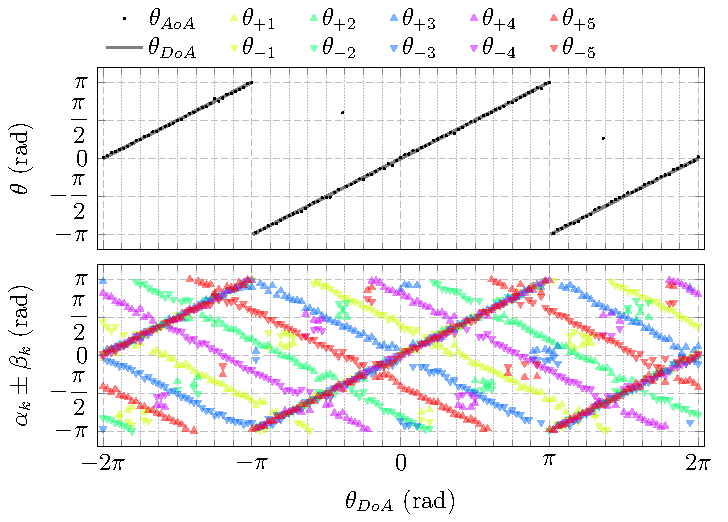
\includegraphics[height=0.785\textheight]{../pictures/simul_POLY_5_R_50_SNR_1_ATT.pdf}
			\caption*{\tiny Fonte: Autor, saída gráfica disponível em \href{https://github.com/HeckRodSav/TG/blob/main/documentation/pictures/POLY_5/simul_POLY_5_R_50_SNR_1_ATT.gif}{\underline{GitHub}}.}
		\end{figure}
	\end{frame}

\subsection{Setes antenas}
	\begin{frame}{R\textsuperscript{2} para sete antenas}
		\begin{table}
			\centering
			\begin{tabular}{@{}
			S[table-format = 3.1]
			S[table-format = 3.2, table-model-setup = \bfseries]
			S[table-format = 3.2, table-model-setup = \bfseries]
			@{}}
			\toprule
			{SNR (\unit{\deci\bel})} & {R\textsuperscript{2} sem ATT (\unit{\percent})} & {R\textsuperscript{2} com ATT (\unit{\percent})}
			\\\midrule
			\infinity & \bfseries 100.00 & 100.00\\
			20 & 84.25 & 100.00\\
			17 & 100.00 & 84.24\\
			14 & 91.90 & 100.00\\
			7 & 99.99 & 84.28\\
			0 & \bfseries 80.15 & \bfseries 99.98\\
			\bottomrule
		\end{tabular}
		\caption*{\tiny Fonte: Autor, saídas das simulações disponíveis em \href{https://github.com/HeckRodSav/TG/tree/main/documentation/data/POLY_7}{\underline{GitHub}}.}
	\end{table}
	\end{frame}

	\begin{frame}
		\begin{figure}
			\centering
			\caption*{Caso ideal ($\text{SNR} \rightarrow \qty{\infinity}{\deci\bel}$).}
			% \begin{tikzpicture}
    % \pgfsetfillopacity{0.5}

    \def\fileName{simul_POLY_7_R_50}
    % \def\fileAddress{../../code/simul/Output/POLY_7/\fileName.dat}
    \def\fileAddress{../data/POLY_7/\fileName.dat}
    % \def\fileAddress{../data/\fileName.dat}

    \def\height{.225\linewidth}
    \def\width{0.75\linewidth}
    \def\distance{0.25cm}
    \def\xmin{-1}
    \def\xmax{101}

    \begin{axis} %configuração do eixo Y esquerdo e eixo X
    [
        name=plot1,
        reverse legend, % inverte a ordem que os items aparecem na legenda
    	% legend style={
        % 	at=(current bounding box.north),
        % 	anchor=south,
        % 	legend columns=6,
        % 	transpose legend,
        % 	draw=none,
        % 	/tikz/every even column/.append style={column sep=0.5cm}
    	% }, % onde exibir
        % axis x line=center,
        % axis y line=center,
        height=\height, % altura da região do gráfico
        width=\width, % largura da região do gráfico
        scale only axis, %
        minor grid style={densely dotted}, % estilo da grade secundária
        major grid style={densely dashed}, % estilo da grade principal
        grid style={lightgray, thin}, % cor das grades
        % axis on top, % forçar grade para ficar por cima do gráfico
        %
        %
        % axis y line*=left, % define gráfico para usar eixo esquerdo sem exibir direito
        y tick label style={
            /pgf/number format/.cd,
            fixed,
            % fixed zerofill,
            precision=1, % quantidade de casas depois da virgula
            /tikz/.cd
        },
        % y filter/.expression={y==0 ? NaN : y},
        scaled y ticks = false,
        ylabel={$\alpha_{k}\pm \beta_{k}$ (\si{\radian})}, % titulo eixo vertical
        % yticklabel={\pgfmathparse{\tick-50}\pgfmathprintnumber{\pgfmathresult}}, % fator multiplicativo para valores do eixo
        y tick label style={/pgf/number format/1000 sep=}, % Altera marcação de milhar
        % yticklabel style={rotate=90},
		ytick={-3.1415, -1.5708, 0, 1.5708, 3.1415},
		yticklabels={$-\pi$,$-\dfrac{\pi}{2}$,$0$,$\dfrac{\pi}{2}$,$\pi$},
        % ytick={0,1,2,3,4,5}, % lista de valores a serem utilizados no eixo
        % ymin=-1,  ymax=4,  % intervalo de valores no eixo y -> na dúvida, deixe comentado
        %
        ymajorgrids=true, % exibir grade principal y
        yminorgrids=true, % exibir grade secundária y
        minor y tick num=4, % contagem de linhas na grade secundária y
        % ybar,
        %
        %
        xlabel={$\theta_{DoA}$ (\si{\radian})}, % título eixo horizontal
        % xticklabel={\pgfmathparse{\tick-50}\pgfmathprintnumber{\pgfmathresult}}, % fator multiplicativo para valores do eixo
        % xticklabels={}, % fator multiplicativo para valores do eixo
		% xtick={0, 12.5, 25, 37.5, 50, 62.6, 75, 87.5, 100},
		% xticklabels={$-2~\pi$,$-\dfrac{3~\pi}{2}$,$-\pi$,$-\dfrac{\pi}{2}$,$0$,$-\dfrac{\pi}{2}$,$\pi$,$-\dfrac{3~\pi}{2}$,$2~\pi$},
		xtick={0, 25, 50, 75, 100},
		xticklabels={$-2 \pi$,$-\pi$,$0$,$\pi$,$2 \pi$},
        % xmode=log,
        % log ticks with fixed point,
        % x filter/.code=\pgfmathparse{#1 + 6.90775527898214},
        x tick label style={
            /pgf/number format/.cd,
            fixed,
            % fixed zerofill,
            precision=1,
            /tikz/.cd,
            /pgf/number format/use comma
        },
        xmin=\xmin, xmax=\xmax, % intervalo de valores no eixo x -> na dúvida, deixe comentado
        scaled x ticks = false,
        %
        xmajorgrids=true, % exibir grade principal x
        xminorgrids=true, % exibir grade secundária x
        minor x tick num=7, % contagem de linhas na grade secundária x
        %
        %
        %
        % unbounded coords=jump,
        % jump threshold/.initial=0.25
    ]

	\addplot[
        antena_7_1,
        mark=triangle*,
		opacity=0.5,
        only marks,
        % smooth
    ] table [
        % col sep=comma,
        x=percent, % cabeçalho da coluna de dados X no arquivo
        y=delta_1_x_7, % cabeçalho da coluna de dados Y no arquivo
    ]
    {\fileAddress};	\label{\fileName.1.1}

    \addplot[
        antena_7_1,
        mark=triangle*,
		opacity=0.5,
		mark options={rotate=180},
        only marks,
        % smooth
    ] table [
        % col sep=comma,
        x=percent, % cabeçalho da coluna de dados X no arquivo
        y=delta_7_x_1, % cabeçalho da coluna de dados Y no arquivo
    ]
    {\fileAddress};	\label{\fileName.1.2}

	\addplot[
        antena_7_2,
        mark=triangle*,
		opacity=0.5,
        only marks,
        % smooth
    ] table [
        % col sep=comma,
        x=percent, % cabeçalho da coluna de dados X no arquivo
        y=delta_2_x_1, % cabeçalho da coluna de dados Y no arquivo
    ]
    {\fileAddress};	\label{\fileName.1.3}

    \addplot[
        antena_7_2,
        mark=triangle*,
		opacity=0.5,
		mark options={rotate=180},
        only marks,
        % smooth
    ] table [
        % col sep=comma,
        x=percent, % cabeçalho da coluna de dados X no arquivo
        y=delta_1_x_2, % cabeçalho da coluna de dados Y no arquivo
    ]
    {\fileAddress};	\label{\fileName.1.4}

	\addplot[
        antena_7_3,
        mark=triangle*,
		opacity=0.5,
        only marks,
        % smooth
    ] table [
        % col sep=comma,
        x=percent, % cabeçalho da coluna de dados X no arquivo
        y=delta_3_x_2, % cabeçalho da coluna de dados Y no arquivo
    ]
    {\fileAddress};	\label{\fileName.1.5}

    \addplot[
        antena_7_3,
        mark=triangle*,
		opacity=0.5,
		mark options={rotate=180},
        only marks,
        % smooth
    ] table [
        % col sep=comma,
        x=percent, % cabeçalho da coluna de dados X no arquivo
        y=delta_2_x_3, % cabeçalho da coluna de dados Y no arquivo
    ]
    {\fileAddress};	\label{\fileName.1.6}

	\addplot[
        antena_7_4,
        mark=triangle*,
		opacity=0.5,
        only marks,
        % smooth
    ] table [
        % col sep=comma,
        x=percent, % cabeçalho da coluna de dados X no arquivo
        y=delta_4_x_3, % cabeçalho da coluna de dados Y no arquivo
    ]
    {\fileAddress};	\label{\fileName.1.7}

    \addplot[
        antena_7_4,
        mark=triangle*,
		opacity=0.5,
		mark options={rotate=180},
        only marks,
        % smooth
    ] table [
        % col sep=comma,
        x=percent, % cabeçalho da coluna de dados X no arquivo
        y=delta_3_x_4, % cabeçalho da coluna de dados Y no arquivo
    ]
    {\fileAddress};	\label{\fileName.1.8}

	\addplot[
        antena_7_5,
        mark=triangle*,
		opacity=0.5,
        only marks,
        % smooth
    ] table [
        % col sep=comma,
        x=percent, % cabeçalho da coluna de dados X no arquivo
        y=delta_5_x_4, % cabeçalho da coluna de dados Y no arquivo
    ]
    {\fileAddress};	\label{\fileName.1.9}

    \addplot[
        antena_7_5,
        mark=triangle*,
		opacity=0.5,
		mark options={rotate=180},
        only marks,
        % smooth
    ] table [
        % col sep=comma,
        x=percent, % cabeçalho da coluna de dados X no arquivo
        y=delta_4_x_5, % cabeçalho da coluna de dados Y no arquivo
    ]
    {\fileAddress};	\label{\fileName.1.10}

	\addplot[
        antena_7_6,
        mark=triangle*,
		opacity=0.5,
        only marks,
        % smooth
    ] table [
        % col sep=comma,
        x=percent, % cabeçalho da coluna de dados X no arquivo
        y=delta_6_x_5, % cabeçalho da coluna de dados Y no arquivo
    ]
    {\fileAddress};	\label{\fileName.1.11}

    \addplot[
        antena_7_6,
        mark=triangle*,
		opacity=0.5,
		mark options={rotate=180},
        only marks,
        % smooth
    ] table [
        % col sep=comma,
        x=percent, % cabeçalho da coluna de dados X no arquivo
        y=delta_5_x_6 % cabeçalho da coluna de dados Y no arquivo
    ]
    {\fileAddress};	\label{\fileName.1.12}

	\addplot[
        antena_7_7,
        mark=triangle*,
		opacity=0.5,
        only marks,
        % smooth
    ] table [
        % col sep=comma,
        x=percent, % cabeçalho da coluna de dados X no arquivo
        y=delta_7_x_6, % cabeçalho da coluna de dados Y no arquivo
    ]
    {\fileAddress};	\label{\fileName.1.13}

    \addplot[
        antena_7_7,
        mark=triangle*,
		opacity=0.5,
		mark options={rotate=180},
        only marks,
        % smooth
    ] table [
        % col sep=comma,
        x=percent, % cabeçalho da coluna de dados X no arquivo
        y=delta_6_x_7, % cabeçalho da coluna de dados Y no arquivo
    ]
    {\fileAddress};	\label{\fileName.1.14}

    \end{axis}

    % \begin{axis} %configuração do eixo Y direito e legenda
    % [
    %     legend cell align=left, % alinhamento de texto na legenda
    %     % legend pos={outer north east}, % onde exibir caixa de legenda
    %     % reverse legend, % inverte a ordem que os items aparecem na legenda
    % 	legend style={
    %     	at=(current bounding box.north),
    %     	anchor=south,
    %     	legend columns=2,
    %     % 	transpose legend,
    %     	draw=none
    % 	}, % onde exibir
    %     % axis x line=center,
    %     % axis y line=center,
    %     height=\height, % altura da região do gráfico
    %     width=\width, % largura da região do gráfico
    %     scale only axis, %
    %     minor grid style={densely dotted}, % estilo da grade secundária
    %     major grid style={densely dashed}, % estilo da grade principal
    %     grid style={lightgray, thin}, % cor das grades
    %     % axis on top, % forçar grade para ficar por cima do gráfico
    %     %
    %     %
    %     axis y line*=right, % define gráfico para usar eixo direito sem exibir esquerdo
    %     ylabel={$V_{out}$ (\si{\milli\volt})}, % titulo eixo vertical
    %     y tick label style={
    %         /pgf/number format/.cd,
    %         fixed,
    %         % fixed zerofill,
    %         precision=3, % quantidade de casas depois da virgula
    %         /tikz/.cd,
    %         /pgf/number format/use comma
    %     },
    %     % y filter/.expression={y==0 ? NaN : y},
    %     scaled y ticks = false,
    %     % yticklabel={\pgfmathparse{\tick*10^3}\pgfmathprintnumber{\pgfmathresult}}, % fator multiplicativo para valores do eixo
    %     y tick label style={/pgf/number format/1000 sep=}, % Altera marcação de milhar
    %     % yticklabel style={rotate=90},
    %     % ytick={-12,-6,0,6,12}, % lista de valores a serem utilizados no eixo
    %     % ymin=0.76503, ymax=0.76509,  % intervalo de valores no eixo y -> na dúvida, deixe comentado
    %     %
    %     ymajorgrids=false, % exibir grade principal y
    %     yminorgrids=false, % exibir grade secundária y
    %     minor y tick num=4, % contagem de linhas na grade secundária y
    %     % ybar,
    %     %
    %     %
    %     axis x line=none, %oculta eixo inferior quando o gráfico anterior já exibe
    %     % xlabel={Frequência (\si{\hertz})}, % título eixo horizontal
    %     % xticklabel={\pgfmathparse{\tick*10^3}\pgfmathprintnumber{\pgfmathresult}}, % fator multiplicativo para valores do eixo
    %     % xmode=log,
    %     % log ticks with fixed point,
    %     % x filter/.code=\pgfmathparse{#1 + 6.90775527898214},
    %     % x tick label style={
    %     %     /pgf/number format/.cd,
    %     %     fixed,
    %     %     % fixed zerofill,
    %     %     precision=0,
    %     %     /tikz/.cd,
    %     %     /pgf/number format/use comma
    %     % },
    %     xmin=\xmin, xmax=\xmax, % intervalo de valores no eixo x -> na dúvida, deixe comentado
    %     % scaled x ticks = true,
    %     %
    %     % xmajorgrids=true, % exibir grade principal x
    %     % xminorgrids=true, % exibir grade secundária x
    %     % minor x tick num=7, % contagem de linhas na grade secundária x
    %     %
    %     %
    %     %
    % ]



    % \addplot[mark=none,red, thick]
    % table [
    %     x=time, % cabeçalho da coluna de dados X no arquivo
    %     y=vout % cabeçalho da coluna de dados Y no arquivo
    % ]
    % {graficos/dados/booster.dat};  \label{\fileName.1.2}

    % % \addlegendimage{/pgfplots/refstyle=_1_2}

    % % \addplot[ForestGreen, densely dashdotted, thick]
    % % coordinates
    % % {
    % %     (\pgfkeysvalueof{/pgfplots/xmin},12)
    % %     (\pgfkeysvalueof{/pgfplots/xmax},12)
    % % };
    % % % \addlegendentry{$V_{out}=\pm\SI{12}{\volt}$}

    % % \addplot[ForestGreen, densely dashdotted, thick]
    % % coordinates
    % % {
    % %     (\pgfkeysvalueof{/pgfplots/xmin},-12)
    % %     (\pgfkeysvalueof{/pgfplots/xmax},-12)
    % % };

    % \end{axis}

    \begin{axis} %configuração do eixo Y esquerdo e eixo X
    [
        at={($(plot1.north)+(0,\distance)$)},
        anchor=south,
        % reverse legend, % inverte a ordem que os items aparecem na legenda
		legend style={
        	at=(current bounding box.north),
        	anchor=south,
        	legend columns=2,
        	transpose legend,
        	draw=none,
        	/tikz/every even column/.append style={column sep=0.5cm}
    	}, % onde exibir
        samples=505,
        domain=0:100,
        % axis x line=center,
        % axis y line=center,
        height=\height, % altura da região do gráfico
        width=\width, % largura da região do gráfico
        scale only axis, %
        minor grid style={densely dotted}, % estilo da grade secundária
        major grid style={densely dashed}, % estilo da grade principal
        grid style={lightgray, thin}, % cor das grades
        % axis on top, % forçar grade para ficar por cima do gráfico
        %
        %
        % axis y line*=left, % define gráfico para usar eixo esquerdo sem exibir direito
        y tick label style={
            /pgf/number format/.cd,
            fixed,
            % fixed zerofill,
            precision=1, % quantidade de casas depois da virgula
            /tikz/.cd
        },
        % y filter/.expression={y==0 ? NaN : y},
        scaled y ticks = false,
        ylabel={$\theta$ (\si{\radian})}, % titulo eixo vertical
        % yticklabel={\pgfmathparse{\tick*10^3}\pgfmathprintnumber{\pgfmathresult}}, % fator multiplicativo para valores do eixo
        y tick label style={/pgf/number format/1000 sep=}, % Altera marcação de milhar
        % yticklabel style={rotate=90},
		ytick={-3.1415, -1.5708, 0, 1.5708, 3.1415},
		yticklabels={$-\pi$,$-\dfrac{\pi}{2}$,$0$,$\dfrac{\pi}{2}$,$\pi$},
        % ytick={0,1,2,3,4,5}, % lista de valores a serem utilizados no eixo
        % ymin=-1,  ymax=4,  % intervalo de valores no eixo y -> na dúvida, deixe comentado
        %
        ymajorgrids=true, % exibir grade principal y
        yminorgrids=true, % exibir grade secundária y
        minor y tick num=4, % contagem de linhas na grade secundária y
        % ybar,
        %
        %
        % xlabel={Tempo (\si{\milli\second})}, % título eixo horizontal
        % xticklabel={\pgfmathparse{\tick*10^3}\pgfmathprintnumber{\pgfmathresult}}, % fator multiplicativo para valores do eixo
		xtick={0, 25, 50, 75, 100},
        xticklabels={}, % fator multiplicativo para valores do eixo
        % xmode=log,
        % log ticks with fixed point,
        % x filter/.code=\pgfmathparse{#1 + 6.90775527898214},
        x tick label style={
            /pgf/number format/.cd,
            fixed,
            % fixed zerofill,
            precision=1,
            /tikz/.cd,
            /pgf/number format/use comma
        },
        xmin=\xmin, xmax=\xmax, % intervalo de valores no eixo x -> na dúvida, deixe comentado
        scaled x ticks = false,
        %
        xmajorgrids=true, % exibir grade principal x
        xminorgrids=true, % exibir grade secundária x
        minor x tick num=7, % contagem de linhas na grade secundária x
        %
        %
        %
        unbounded coords=jump,
		jump threshold/.initial=0.01
    ]


    \addplot[
        Black,
        mark=*,
		mark size=0.5pt,
        only marks,
        % smooth
    ] table [
        % col sep=comma,
        x=percent, % cabeçalho da coluna de dados X no arquivo
        y=choose_angle, % cabeçalho da coluna de dados Y no arquivo
	]
	{\fileAddress};	\addlegendentry{$\theta_{AoA}$}

	% \addplot[
	% 	Black,
	% 	mark=o,
	% 	mark size=1.5pt,
	% 	only marks,
	% 	opacity=0.5,
    %     thick,
	% 	% smooth
	% ] table [
	% 	% col sep=comma,
	% 	x=percent, % cabeçalho da coluna de dados X no arquivo
	% 	y=ang_W, % cabeçalho da coluna de dados Y no arquivo
	% ]
	% {\fileAddress};
    \addplot [
        Black,
        opacity=0.5,
        mark=none,
        mark size=5pt,
        very thick,
        % only marks,
        % smooth
    ] {((x==25)||(x==75)?nan:pi*(mod(x+25,50)-25)/25)};
    \addlegendentry{$\theta_{DoA}$}


	\addlegendimage{/pgfplots/refstyle=\fileName.1.1}\addlegendentry{$\theta_{+1}$}
	\addlegendimage{/pgfplots/refstyle=\fileName.1.2}\addlegendentry{$\theta_{-1}$}

	\addlegendimage{/pgfplots/refstyle=\fileName.1.3}\addlegendentry{$\theta_{+2}$}
	\addlegendimage{/pgfplots/refstyle=\fileName.1.4}\addlegendentry{$\theta_{-2}$}

    \addlegendimage{/pgfplots/refstyle=\fileName.1.5}\addlegendentry{$\theta_{+3}$}
	\addlegendimage{/pgfplots/refstyle=\fileName.1.6}\addlegendentry{$\theta_{-3}$}

    \addlegendimage{/pgfplots/refstyle=\fileName.1.7}\addlegendentry{$\theta_{+4}$}
	\addlegendimage{/pgfplots/refstyle=\fileName.1.8}\addlegendentry{$\theta_{-4}$}

    \addlegendimage{/pgfplots/refstyle=\fileName.1.9}\addlegendentry{$\theta_{+5}$}
	\addlegendimage{/pgfplots/refstyle=\fileName.1.10}\addlegendentry{$\theta_{-5}$}

    \addlegendimage{/pgfplots/refstyle=\fileName.1.11}\addlegendentry{$\theta_{+6}$}
	\addlegendimage{/pgfplots/refstyle=\fileName.1.12}\addlegendentry{$\theta_{-6}$}

    \addlegendimage{/pgfplots/refstyle=\fileName.1.13}\addlegendentry{$\theta_{+7}$}
	\addlegendimage{/pgfplots/refstyle=\fileName.1.14}\addlegendentry{$\theta_{-7}$}


    \end{axis}

    % \begin{axis} %configuração do eixo Y direito e legenda
    % [
    %     at={($(plot1.north)+(0,\distance)$)},
    %     anchor=south,
    %     legend cell align=left, % alinhamento de texto na legenda
    %     % legend pos={outer north east}, % onde exibir caixa de legenda
    %     % reverse legend, % inverte a ordem que os items aparecem na legenda
    % 	legend style={
    %     	at=(current bounding box.north),
    %     	anchor=south,
    %     	legend columns=3,
    %     % 	transpose legend,
    %     	draw=none,
    %     	/tikz/every even column/.append style={column sep=0.5cm}
    % 	}, % onde exibir
    %     % axis x line=center,
    %     % axis y line=center,
    %     height=\height, % altura da região do gráfico
    %     width=\width, % largura da região do gráfico
    %     scale only axis, %
    %     minor grid style={densely dotted}, % estilo da grade secundária
    %     major grid style={densely dashed}, % estilo da grade principal
    %     grid style={lightgray, thin}, % cor das grades
    %     % axis on top, % forçar grade para ficar por cima do gráfico
    %     %
    %     %
    %     axis y line*=right, % define gráfico para usar eixo direito sem exibir esquerdo
    %     ylabel={$V_{out}$ (\si{\volt})}, % titulo eixo vertical
    %     y tick label style={
    %         /pgf/number format/.cd,
    %         fixed,
    %         % fixed zerofill,
    %         precision=3, % quantidade de casas depois da virgula
    %         /tikz/.cd,
    %         /pgf/number format/use comma
    %     },
    %     % y filter/.expression={y==0 ? NaN : y},
    %     scaled y ticks = false,
    %     % yticklabel={\pgfmathparse{\tick*10^3}\pgfmathprintnumber{\pgfmathresult}}, % fator multiplicativo para valores do eixo
    %     y tick label style={/pgf/number format/1000 sep=}, % Altera marcação de milhar
    %     % yticklabel style={rotate=90},
    %     % ytick={-12,-6,0,6,12}, % lista de valores a serem utilizados no eixo
    %     % ymin=0.76503, ymax=0.76509,  % intervalo de valores no eixo y -> na dúvida, deixe comentado
    %     %
    %     ymajorgrids=false, % exibir grade principal y
    %     yminorgrids=false, % exibir grade secundária y
    %     minor y tick num=4, % contagem de linhas na grade secundária y
    %     % ybar,
    %     %
    %     %
    %     axis x line=none, %oculta eixo inferior quando o gráfico anterior já exibe
    %     % xlabel={Frequência (\si{\hertz})}, % título eixo horizontal
    %     % xticklabel={\pgfmathparse{\tick*10^3}\pgfmathprintnumber{\pgfmathresult}}, % fator multiplicativo para valores do eixo
    %     % xmode=log,
    %     % log ticks with fixed point,
    %     % x filter/.code=\pgfmathparse{#1 + 6.90775527898214},
    %     % x tick label style={
    %     %     /pgf/number format/.cd,
    %     %     fixed,
    %     %     % fixed zerofill,
    %     %     precision=0,
    %     %     /tikz/.cd,
    %     %     /pgf/number format/use comma
    %     % },
    %     xmin=\xmin, xmax=\xmax, % intervalo de valores no eixo x -> na dúvida, deixe comentado
    %     % scaled x ticks = true,
    %     %
    %     % xmajorgrids=true, % exibir grade principal x
    %     % xminorgrids=true, % exibir grade secundária x
    %     % minor x tick num=10, % contagem de linhas na grade secundária x
    %     %
    %     %
    %     %
    % ]


    % \addlegendimage{/pgfplots/refstyle=_2_1}\addlegendentry{$V_{in}$}
    % \addlegendimage{/pgfplots/refstyle=_2_2}\addlegendentry{$V_{in}$}
    % % \addplot[mark=none,red, thick]
    % % table [
    % %     x=time, % cabeçalho da coluna de dados X no arquivo
    % %     y=vout % cabeçalho da coluna de dados Y no arquivo
    % % ]
    % % {graficos/dados/booster.dat}; % \label{\fileName.1.2}
    % % \addlegendentry{$V_{out}$}

    % \addlegendimage{/pgfplots/refstyle=_1_1}\addlegendentry{$I_{out}$}
    % \addlegendimage{/pgfplots/refstyle=_1_2}\addlegendentry{$I_{out}$}

    % % \addlegendimage{/pgfplots/refstyle=_1_2}

    % % \addplot[ForestGreen, densely dashdotted, thick]
    % % coordinates
    % % {
    % %     (\pgfkeysvalueof{/pgfplots/xmin},12)
    % %     (\pgfkeysvalueof{/pgfplots/xmax},12)
    % % };
    % % % \addlegendentry{$V_{out}=\pm\SI{12}{\volt}$}

    % % \addplot[ForestGreen, densely dashdotted, thick]
    % % coordinates
    % % {
    % %     (\pgfkeysvalueof{/pgfplots/xmin},-12)
    % %     (\pgfkeysvalueof{/pgfplots/xmax},-12)
    % % };

    % \end{axis}



\end{tikzpicture}

			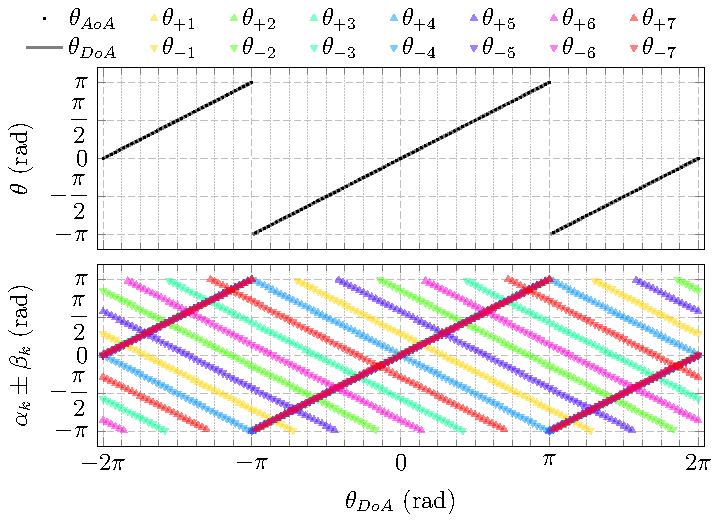
\includegraphics[height=0.785\textheight]{../pictures/simul_POLY_7_R_50.pdf}
			\caption*{\tiny Fonte: Autor, saída gráfica disponível em \href{https://github.com/HeckRodSav/TG/blob/main/documentation/pictures/POLY_7/simul_POLY_7_R_50.gif}{\underline{GitHub}}.}
		\end{figure}
	\end{frame}
	\begin{frame}
		\begin{figure}
			\centering
			\caption*{Caso $\text{SNR} = \SI{0}{\deci\bel}$, sem atenuação.}
			% \begin{tikzpicture}
    % \pgfsetfillopacity{0.5}

    \def\fileName{simul_POLY_7_R_50_SNR_1}
    % \def\fileAddress{../../code/simul/Output/POLY_7/\fileName.dat}
    \def\fileAddress{../data/POLY_7/\fileName.dat}
    % \def\fileAddress{../data/\fileName.dat}

    \def\height{.225\linewidth}
    \def\width{0.75\linewidth}
    \def\distance{0.25cm}
    \def\xmin{-1}
    \def\xmax{101}

    \begin{axis} %configuração do eixo Y esquerdo e eixo X
    [
        name=plot1,
        reverse legend, % inverte a ordem que os items aparecem na legenda
    	% legend style={
        % 	at=(current bounding box.north),
        % 	anchor=south,
        % 	legend columns=6,
        % 	transpose legend,
        % 	draw=none,
        % 	/tikz/every even column/.append style={column sep=0.5cm}
    	% }, % onde exibir
        % axis x line=center,
        % axis y line=center,
        height=\height, % altura da região do gráfico
        width=\width, % largura da região do gráfico
        scale only axis, %
        minor grid style={densely dotted}, % estilo da grade secundária
        major grid style={densely dashed}, % estilo da grade principal
        grid style={lightgray, thin}, % cor das grades
        % axis on top, % forçar grade para ficar por cima do gráfico
        %
        %
        % axis y line*=left, % define gráfico para usar eixo esquerdo sem exibir direito
        y tick label style={
            /pgf/number format/.cd,
            fixed,
            % fixed zerofill,
            precision=1, % quantidade de casas depois da virgula
            /tikz/.cd
        },
        % y filter/.expression={y==0 ? NaN : y},
        scaled y ticks = false,
        ylabel={$\alpha_{k}\pm \beta_{k}$ (\si{\radian})}, % titulo eixo vertical
        % yticklabel={\pgfmathparse{\tick-50}\pgfmathprintnumber{\pgfmathresult}}, % fator multiplicativo para valores do eixo
        y tick label style={/pgf/number format/1000 sep=}, % Altera marcação de milhar
        % yticklabel style={rotate=90},
		ytick={-3.1415, -1.5708, 0, 1.5708, 3.1415},
		yticklabels={$-\pi$,$-\dfrac{\pi}{2}$,$0$,$\dfrac{\pi}{2}$,$\pi$},
        % ytick={0,1,2,3,4,5}, % lista de valores a serem utilizados no eixo
        % ymin=-1,  ymax=4,  % intervalo de valores no eixo y -> na dúvida, deixe comentado
        %
        ymajorgrids=true, % exibir grade principal y
        yminorgrids=true, % exibir grade secundária y
        minor y tick num=4, % contagem de linhas na grade secundária y
        % ybar,
        %
        %
        xlabel={$\theta_{DoA}$ (\si{\radian})}, % título eixo horizontal
        % xticklabel={\pgfmathparse{\tick-50}\pgfmathprintnumber{\pgfmathresult}}, % fator multiplicativo para valores do eixo
        % xticklabels={}, % fator multiplicativo para valores do eixo
		% xtick={0, 12.5, 25, 37.5, 50, 62.6, 75, 87.5, 100},
		% xticklabels={$-2~\pi$,$-\dfrac{3~\pi}{2}$,$-\pi$,$-\dfrac{\pi}{2}$,$0$,$-\dfrac{\pi}{2}$,$\pi$,$-\dfrac{3~\pi}{2}$,$2~\pi$},
		xtick={0, 25, 50, 75, 100},
		xticklabels={$-2 \pi$,$-\pi$,$0$,$\pi$,$2 \pi$},
        % xmode=log,
        % log ticks with fixed point,
        % x filter/.code=\pgfmathparse{#1 + 6.90775527898214},
        x tick label style={
            /pgf/number format/.cd,
            fixed,
            % fixed zerofill,
            precision=1,
            /tikz/.cd,
            /pgf/number format/use comma
        },
        xmin=\xmin, xmax=\xmax, % intervalo de valores no eixo x -> na dúvida, deixe comentado
        scaled x ticks = false,
        %
        xmajorgrids=true, % exibir grade principal x
        xminorgrids=true, % exibir grade secundária x
        minor x tick num=7, % contagem de linhas na grade secundária x
        %
        %
        %
        % unbounded coords=jump,
        % jump threshold/.initial=0.25
    ]

	\addplot[
        antena_7_1,
        mark=triangle*,
		opacity=0.5,
        only marks,
        % smooth
    ] table [
        % col sep=comma,
        x=percent, % cabeçalho da coluna de dados X no arquivo
        y=delta_1_x_7, % cabeçalho da coluna de dados Y no arquivo
    ]
    {\fileAddress};	\label{\fileName.1.1}

    \addplot[
        antena_7_1,
        mark=triangle*,
		opacity=0.5,
		mark options={rotate=180},
        only marks,
        % smooth
    ] table [
        % col sep=comma,
        x=percent, % cabeçalho da coluna de dados X no arquivo
        y=delta_7_x_1, % cabeçalho da coluna de dados Y no arquivo
    ]
    {\fileAddress};	\label{\fileName.1.2}

	\addplot[
        antena_7_2,
        mark=triangle*,
		opacity=0.5,
        only marks,
        % smooth
    ] table [
        % col sep=comma,
        x=percent, % cabeçalho da coluna de dados X no arquivo
        y=delta_2_x_1, % cabeçalho da coluna de dados Y no arquivo
    ]
    {\fileAddress};	\label{\fileName.1.3}

    \addplot[
        antena_7_2,
        mark=triangle*,
		opacity=0.5,
		mark options={rotate=180},
        only marks,
        % smooth
    ] table [
        % col sep=comma,
        x=percent, % cabeçalho da coluna de dados X no arquivo
        y=delta_1_x_2, % cabeçalho da coluna de dados Y no arquivo
    ]
    {\fileAddress};	\label{\fileName.1.4}

	\addplot[
        antena_7_3,
        mark=triangle*,
		opacity=0.5,
        only marks,
        % smooth
    ] table [
        % col sep=comma,
        x=percent, % cabeçalho da coluna de dados X no arquivo
        y=delta_3_x_2, % cabeçalho da coluna de dados Y no arquivo
    ]
    {\fileAddress};	\label{\fileName.1.5}

    \addplot[
        antena_7_3,
        mark=triangle*,
		opacity=0.5,
		mark options={rotate=180},
        only marks,
        % smooth
    ] table [
        % col sep=comma,
        x=percent, % cabeçalho da coluna de dados X no arquivo
        y=delta_2_x_3, % cabeçalho da coluna de dados Y no arquivo
    ]
    {\fileAddress};	\label{\fileName.1.6}

	\addplot[
        antena_7_4,
        mark=triangle*,
		opacity=0.5,
        only marks,
        % smooth
    ] table [
        % col sep=comma,
        x=percent, % cabeçalho da coluna de dados X no arquivo
        y=delta_4_x_3, % cabeçalho da coluna de dados Y no arquivo
    ]
    {\fileAddress};	\label{\fileName.1.7}

    \addplot[
        antena_7_4,
        mark=triangle*,
		opacity=0.5,
		mark options={rotate=180},
        only marks,
        % smooth
    ] table [
        % col sep=comma,
        x=percent, % cabeçalho da coluna de dados X no arquivo
        y=delta_3_x_4, % cabeçalho da coluna de dados Y no arquivo
    ]
    {\fileAddress};	\label{\fileName.1.8}

	\addplot[
        antena_7_5,
        mark=triangle*,
		opacity=0.5,
        only marks,
        % smooth
    ] table [
        % col sep=comma,
        x=percent, % cabeçalho da coluna de dados X no arquivo
        y=delta_5_x_4, % cabeçalho da coluna de dados Y no arquivo
    ]
    {\fileAddress};	\label{\fileName.1.9}

    \addplot[
        antena_7_5,
        mark=triangle*,
		opacity=0.5,
		mark options={rotate=180},
        only marks,
        % smooth
    ] table [
        % col sep=comma,
        x=percent, % cabeçalho da coluna de dados X no arquivo
        y=delta_4_x_5, % cabeçalho da coluna de dados Y no arquivo
    ]
    {\fileAddress};	\label{\fileName.1.10}

	\addplot[
        antena_7_6,
        mark=triangle*,
		opacity=0.5,
        only marks,
        % smooth
    ] table [
        % col sep=comma,
        x=percent, % cabeçalho da coluna de dados X no arquivo
        y=delta_6_x_5, % cabeçalho da coluna de dados Y no arquivo
    ]
    {\fileAddress};	\label{\fileName.1.11}

    \addplot[
        antena_7_6,
        mark=triangle*,
		opacity=0.5,
		mark options={rotate=180},
        only marks,
        % smooth
    ] table [
        % col sep=comma,
        x=percent, % cabeçalho da coluna de dados X no arquivo
        y=delta_5_x_6 % cabeçalho da coluna de dados Y no arquivo
    ]
    {\fileAddress};	\label{\fileName.1.12}

	\addplot[
        antena_7_7,
        mark=triangle*,
		opacity=0.5,
        only marks,
        % smooth
    ] table [
        % col sep=comma,
        x=percent, % cabeçalho da coluna de dados X no arquivo
        y=delta_7_x_6, % cabeçalho da coluna de dados Y no arquivo
    ]
    {\fileAddress};	\label{\fileName.1.13}

    \addplot[
        antena_7_7,
        mark=triangle*,
		opacity=0.5,
		mark options={rotate=180},
        only marks,
        % smooth
    ] table [
        % col sep=comma,
        x=percent, % cabeçalho da coluna de dados X no arquivo
        y=delta_6_x_7, % cabeçalho da coluna de dados Y no arquivo
    ]
    {\fileAddress};	\label{\fileName.1.14}

    \end{axis}

    % \begin{axis} %configuração do eixo Y direito e legenda
    % [
    %     legend cell align=left, % alinhamento de texto na legenda
    %     % legend pos={outer north east}, % onde exibir caixa de legenda
    %     % reverse legend, % inverte a ordem que os items aparecem na legenda
    % 	legend style={
    %     	at=(current bounding box.north),
    %     	anchor=south,
    %     	legend columns=2,
    %     % 	transpose legend,
    %     	draw=none
    % 	}, % onde exibir
    %     % axis x line=center,
    %     % axis y line=center,
    %     height=\height, % altura da região do gráfico
    %     width=\width, % largura da região do gráfico
    %     scale only axis, %
    %     minor grid style={densely dotted}, % estilo da grade secundária
    %     major grid style={densely dashed}, % estilo da grade principal
    %     grid style={lightgray, thin}, % cor das grades
    %     % axis on top, % forçar grade para ficar por cima do gráfico
    %     %
    %     %
    %     axis y line*=right, % define gráfico para usar eixo direito sem exibir esquerdo
    %     ylabel={$V_{out}$ (\si{\milli\volt})}, % titulo eixo vertical
    %     y tick label style={
    %         /pgf/number format/.cd,
    %         fixed,
    %         % fixed zerofill,
    %         precision=3, % quantidade de casas depois da virgula
    %         /tikz/.cd,
    %         /pgf/number format/use comma
    %     },
    %     % y filter/.expression={y==0 ? NaN : y},
    %     scaled y ticks = false,
    %     % yticklabel={\pgfmathparse{\tick*10^3}\pgfmathprintnumber{\pgfmathresult}}, % fator multiplicativo para valores do eixo
    %     y tick label style={/pgf/number format/1000 sep=}, % Altera marcação de milhar
    %     % yticklabel style={rotate=90},
    %     % ytick={-12,-6,0,6,12}, % lista de valores a serem utilizados no eixo
    %     % ymin=0.76503, ymax=0.76509,  % intervalo de valores no eixo y -> na dúvida, deixe comentado
    %     %
    %     ymajorgrids=false, % exibir grade principal y
    %     yminorgrids=false, % exibir grade secundária y
    %     minor y tick num=4, % contagem de linhas na grade secundária y
    %     % ybar,
    %     %
    %     %
    %     axis x line=none, %oculta eixo inferior quando o gráfico anterior já exibe
    %     % xlabel={Frequência (\si{\hertz})}, % título eixo horizontal
    %     % xticklabel={\pgfmathparse{\tick*10^3}\pgfmathprintnumber{\pgfmathresult}}, % fator multiplicativo para valores do eixo
    %     % xmode=log,
    %     % log ticks with fixed point,
    %     % x filter/.code=\pgfmathparse{#1 + 6.90775527898214},
    %     % x tick label style={
    %     %     /pgf/number format/.cd,
    %     %     fixed,
    %     %     % fixed zerofill,
    %     %     precision=0,
    %     %     /tikz/.cd,
    %     %     /pgf/number format/use comma
    %     % },
    %     xmin=\xmin, xmax=\xmax, % intervalo de valores no eixo x -> na dúvida, deixe comentado
    %     % scaled x ticks = true,
    %     %
    %     % xmajorgrids=true, % exibir grade principal x
    %     % xminorgrids=true, % exibir grade secundária x
    %     % minor x tick num=7, % contagem de linhas na grade secundária x
    %     %
    %     %
    %     %
    % ]



    % \addplot[mark=none,red, thick]
    % table [
    %     x=time, % cabeçalho da coluna de dados X no arquivo
    %     y=vout % cabeçalho da coluna de dados Y no arquivo
    % ]
    % {graficos/dados/booster.dat};  \label{\fileName.1.2}

    % % \addlegendimage{/pgfplots/refstyle=_1_2}

    % % \addplot[ForestGreen, densely dashdotted, thick]
    % % coordinates
    % % {
    % %     (\pgfkeysvalueof{/pgfplots/xmin},12)
    % %     (\pgfkeysvalueof{/pgfplots/xmax},12)
    % % };
    % % % \addlegendentry{$V_{out}=\pm\SI{12}{\volt}$}

    % % \addplot[ForestGreen, densely dashdotted, thick]
    % % coordinates
    % % {
    % %     (\pgfkeysvalueof{/pgfplots/xmin},-12)
    % %     (\pgfkeysvalueof{/pgfplots/xmax},-12)
    % % };

    % \end{axis}

    \begin{axis} %configuração do eixo Y esquerdo e eixo X
    [
        at={($(plot1.north)+(0,\distance)$)},
        anchor=south,
        % reverse legend, % inverte a ordem que os items aparecem na legenda
		legend style={
        	at=(current bounding box.north),
        	anchor=south,
        	legend columns=2,
        	transpose legend,
        	draw=none,
        	/tikz/every even column/.append style={column sep=0.5cm}
    	}, % onde exibir
        samples=505,
        domain=0:100,
        % axis x line=center,
        % axis y line=center,
        height=\height, % altura da região do gráfico
        width=\width, % largura da região do gráfico
        scale only axis, %
        minor grid style={densely dotted}, % estilo da grade secundária
        major grid style={densely dashed}, % estilo da grade principal
        grid style={lightgray, thin}, % cor das grades
        % axis on top, % forçar grade para ficar por cima do gráfico
        %
        %
        % axis y line*=left, % define gráfico para usar eixo esquerdo sem exibir direito
        y tick label style={
            /pgf/number format/.cd,
            fixed,
            % fixed zerofill,
            precision=1, % quantidade de casas depois da virgula
            /tikz/.cd
        },
        % y filter/.expression={y==0 ? NaN : y},
        scaled y ticks = false,
        ylabel={$\theta$ (\si{\radian})}, % titulo eixo vertical
        % yticklabel={\pgfmathparse{\tick*10^3}\pgfmathprintnumber{\pgfmathresult}}, % fator multiplicativo para valores do eixo
        y tick label style={/pgf/number format/1000 sep=}, % Altera marcação de milhar
        % yticklabel style={rotate=90},
		ytick={-3.1415, -1.5708, 0, 1.5708, 3.1415},
		yticklabels={$-\pi$,$-\dfrac{\pi}{2}$,$0$,$\dfrac{\pi}{2}$,$\pi$},
        % ytick={0,1,2,3,4,5}, % lista de valores a serem utilizados no eixo
        % ymin=-1,  ymax=4,  % intervalo de valores no eixo y -> na dúvida, deixe comentado
        %
        ymajorgrids=true, % exibir grade principal y
        yminorgrids=true, % exibir grade secundária y
        minor y tick num=4, % contagem de linhas na grade secundária y
        % ybar,
        %
        %
        % xlabel={Tempo (\si{\milli\second})}, % título eixo horizontal
        % xticklabel={\pgfmathparse{\tick*10^3}\pgfmathprintnumber{\pgfmathresult}}, % fator multiplicativo para valores do eixo
		xtick={0, 25, 50, 75, 100},
        xticklabels={}, % fator multiplicativo para valores do eixo
        % xmode=log,
        % log ticks with fixed point,
        % x filter/.code=\pgfmathparse{#1 + 6.90775527898214},
        x tick label style={
            /pgf/number format/.cd,
            fixed,
            % fixed zerofill,
            precision=1,
            /tikz/.cd,
            /pgf/number format/use comma
        },
        xmin=\xmin, xmax=\xmax, % intervalo de valores no eixo x -> na dúvida, deixe comentado
        scaled x ticks = false,
        %
        xmajorgrids=true, % exibir grade principal x
        xminorgrids=true, % exibir grade secundária x
        minor x tick num=7, % contagem de linhas na grade secundária x
        %
        %
        %
        unbounded coords=jump,
		jump threshold/.initial=0.01
    ]


    \addplot[
        Black,
        mark=*,
		mark size=0.5pt,
        only marks,
        % smooth
    ] table [
        % col sep=comma,
        x=percent, % cabeçalho da coluna de dados X no arquivo
        y=choose_angle, % cabeçalho da coluna de dados Y no arquivo
	]
	{\fileAddress};	\addlegendentry{$\theta_{AoA}$}

	% \addplot[
	% 	Black,
	% 	mark=o,
	% 	mark size=1.5pt,
	% 	only marks,
	% 	opacity=0.5,
    %     thick,
	% 	% smooth
	% ] table [
	% 	% col sep=comma,
	% 	x=percent, % cabeçalho da coluna de dados X no arquivo
	% 	y=ang_W, % cabeçalho da coluna de dados Y no arquivo
	% ]
	% {\fileAddress};
    \addplot [
        Black,
        opacity=0.5,
        mark=none,
        mark size=5pt,
        very thick,
        % only marks,
        % smooth
    ] {((x==25)||(x==75)?nan:pi*(mod(x+25,50)-25)/25)};
    \addlegendentry{$\theta_{DoA}$}


	\addlegendimage{/pgfplots/refstyle=\fileName.1.1}\addlegendentry{$\theta_{+1}$}
	\addlegendimage{/pgfplots/refstyle=\fileName.1.2}\addlegendentry{$\theta_{-1}$}

	\addlegendimage{/pgfplots/refstyle=\fileName.1.3}\addlegendentry{$\theta_{+2}$}
	\addlegendimage{/pgfplots/refstyle=\fileName.1.4}\addlegendentry{$\theta_{-2}$}

    \addlegendimage{/pgfplots/refstyle=\fileName.1.5}\addlegendentry{$\theta_{+3}$}
	\addlegendimage{/pgfplots/refstyle=\fileName.1.6}\addlegendentry{$\theta_{-3}$}

    \addlegendimage{/pgfplots/refstyle=\fileName.1.7}\addlegendentry{$\theta_{+4}$}
	\addlegendimage{/pgfplots/refstyle=\fileName.1.8}\addlegendentry{$\theta_{-4}$}

    \addlegendimage{/pgfplots/refstyle=\fileName.1.9}\addlegendentry{$\theta_{+5}$}
	\addlegendimage{/pgfplots/refstyle=\fileName.1.10}\addlegendentry{$\theta_{-5}$}

    \addlegendimage{/pgfplots/refstyle=\fileName.1.11}\addlegendentry{$\theta_{+6}$}
	\addlegendimage{/pgfplots/refstyle=\fileName.1.12}\addlegendentry{$\theta_{-6}$}

    \addlegendimage{/pgfplots/refstyle=\fileName.1.13}\addlegendentry{$\theta_{+7}$}
	\addlegendimage{/pgfplots/refstyle=\fileName.1.14}\addlegendentry{$\theta_{-7}$}


    \end{axis}

    % \begin{axis} %configuração do eixo Y direito e legenda
    % [
    %     at={($(plot1.north)+(0,\distance)$)},
    %     anchor=south,
    %     legend cell align=left, % alinhamento de texto na legenda
    %     % legend pos={outer north east}, % onde exibir caixa de legenda
    %     % reverse legend, % inverte a ordem que os items aparecem na legenda
    % 	legend style={
    %     	at=(current bounding box.north),
    %     	anchor=south,
    %     	legend columns=3,
    %     % 	transpose legend,
    %     	draw=none,
    %     	/tikz/every even column/.append style={column sep=0.5cm}
    % 	}, % onde exibir
    %     % axis x line=center,
    %     % axis y line=center,
    %     height=\height, % altura da região do gráfico
    %     width=\width, % largura da região do gráfico
    %     scale only axis, %
    %     minor grid style={densely dotted}, % estilo da grade secundária
    %     major grid style={densely dashed}, % estilo da grade principal
    %     grid style={lightgray, thin}, % cor das grades
    %     % axis on top, % forçar grade para ficar por cima do gráfico
    %     %
    %     %
    %     axis y line*=right, % define gráfico para usar eixo direito sem exibir esquerdo
    %     ylabel={$V_{out}$ (\si{\volt})}, % titulo eixo vertical
    %     y tick label style={
    %         /pgf/number format/.cd,
    %         fixed,
    %         % fixed zerofill,
    %         precision=3, % quantidade de casas depois da virgula
    %         /tikz/.cd,
    %         /pgf/number format/use comma
    %     },
    %     % y filter/.expression={y==0 ? NaN : y},
    %     scaled y ticks = false,
    %     % yticklabel={\pgfmathparse{\tick*10^3}\pgfmathprintnumber{\pgfmathresult}}, % fator multiplicativo para valores do eixo
    %     y tick label style={/pgf/number format/1000 sep=}, % Altera marcação de milhar
    %     % yticklabel style={rotate=90},
    %     % ytick={-12,-6,0,6,12}, % lista de valores a serem utilizados no eixo
    %     % ymin=0.76503, ymax=0.76509,  % intervalo de valores no eixo y -> na dúvida, deixe comentado
    %     %
    %     ymajorgrids=false, % exibir grade principal y
    %     yminorgrids=false, % exibir grade secundária y
    %     minor y tick num=4, % contagem de linhas na grade secundária y
    %     % ybar,
    %     %
    %     %
    %     axis x line=none, %oculta eixo inferior quando o gráfico anterior já exibe
    %     % xlabel={Frequência (\si{\hertz})}, % título eixo horizontal
    %     % xticklabel={\pgfmathparse{\tick*10^3}\pgfmathprintnumber{\pgfmathresult}}, % fator multiplicativo para valores do eixo
    %     % xmode=log,
    %     % log ticks with fixed point,
    %     % x filter/.code=\pgfmathparse{#1 + 6.90775527898214},
    %     % x tick label style={
    %     %     /pgf/number format/.cd,
    %     %     fixed,
    %     %     % fixed zerofill,
    %     %     precision=0,
    %     %     /tikz/.cd,
    %     %     /pgf/number format/use comma
    %     % },
    %     xmin=\xmin, xmax=\xmax, % intervalo de valores no eixo x -> na dúvida, deixe comentado
    %     % scaled x ticks = true,
    %     %
    %     % xmajorgrids=true, % exibir grade principal x
    %     % xminorgrids=true, % exibir grade secundária x
    %     % minor x tick num=10, % contagem de linhas na grade secundária x
    %     %
    %     %
    %     %
    % ]


    % \addlegendimage{/pgfplots/refstyle=_2_1}\addlegendentry{$V_{in}$}
    % \addlegendimage{/pgfplots/refstyle=_2_2}\addlegendentry{$V_{in}$}
    % % \addplot[mark=none,red, thick]
    % % table [
    % %     x=time, % cabeçalho da coluna de dados X no arquivo
    % %     y=vout % cabeçalho da coluna de dados Y no arquivo
    % % ]
    % % {graficos/dados/booster.dat}; % \label{\fileName.1.2}
    % % \addlegendentry{$V_{out}$}

    % \addlegendimage{/pgfplots/refstyle=_1_1}\addlegendentry{$I_{out}$}
    % \addlegendimage{/pgfplots/refstyle=_1_2}\addlegendentry{$I_{out}$}

    % % \addlegendimage{/pgfplots/refstyle=_1_2}

    % % \addplot[ForestGreen, densely dashdotted, thick]
    % % coordinates
    % % {
    % %     (\pgfkeysvalueof{/pgfplots/xmin},12)
    % %     (\pgfkeysvalueof{/pgfplots/xmax},12)
    % % };
    % % % \addlegendentry{$V_{out}=\pm\SI{12}{\volt}$}

    % % \addplot[ForestGreen, densely dashdotted, thick]
    % % coordinates
    % % {
    % %     (\pgfkeysvalueof{/pgfplots/xmin},-12)
    % %     (\pgfkeysvalueof{/pgfplots/xmax},-12)
    % % };

    % \end{axis}



\end{tikzpicture}

			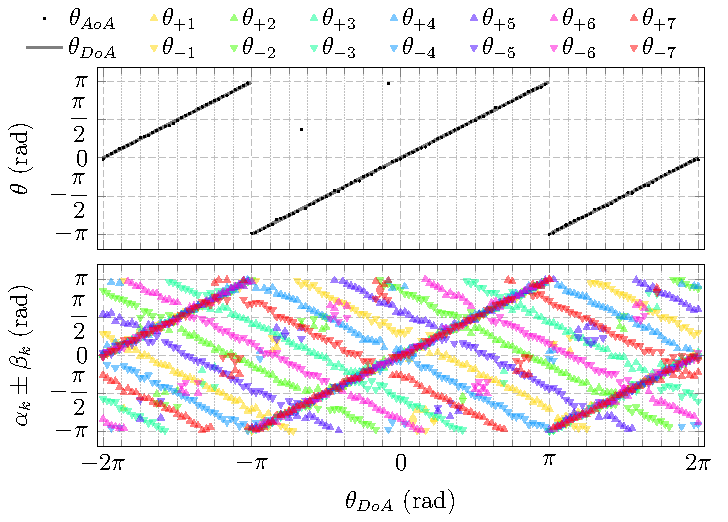
\includegraphics[height=0.785\textheight]{../pictures/simul_POLY_7_R_50_SNR_1.pdf}
			\caption*{\tiny Fonte: Autor, saída gráfica disponível em \href{https://github.com/HeckRodSav/TG/blob/main/documentation/pictures/POLY_7/simul_POLY_7_R_50_SNR_1.gif}{\underline{GitHub}}.}
		\end{figure}
	\end{frame}
	\begin{frame}
		\begin{figure}
			\centering
			\caption*{Caso $\text{SNR} = \SI{0}{\deci\bel}$, com atenuação.}
			% \begin{tikzpicture}
    % \pgfsetfillopacity{0.5}

    \def\fileName{simul_POLY_7_R_50_SNR_1_ATT}
    % \def\fileAddress{../../code/simul/Output/POLY_7/\fileName.dat}
    \def\fileAddress{../data/POLY_7/\fileName.dat}
    % \def\fileAddress{../data/\fileName.dat}

    \def\height{.225\linewidth}
    \def\width{0.75\linewidth}
    \def\distance{0.25cm}
    \def\xmin{-1}
    \def\xmax{101}

    \begin{axis} %configuração do eixo Y esquerdo e eixo X
    [
        name=plot1,
        reverse legend, % inverte a ordem que os items aparecem na legenda
    	% legend style={
        % 	at=(current bounding box.north),
        % 	anchor=south,
        % 	legend columns=6,
        % 	transpose legend,
        % 	draw=none,
        % 	/tikz/every even column/.append style={column sep=0.5cm}
    	% }, % onde exibir
        % axis x line=center,
        % axis y line=center,
        height=\height, % altura da região do gráfico
        width=\width, % largura da região do gráfico
        scale only axis, %
        minor grid style={densely dotted}, % estilo da grade secundária
        major grid style={densely dashed}, % estilo da grade principal
        grid style={lightgray, thin}, % cor das grades
        % axis on top, % forçar grade para ficar por cima do gráfico
        %
        %
        % axis y line*=left, % define gráfico para usar eixo esquerdo sem exibir direito
        y tick label style={
            /pgf/number format/.cd,
            fixed,
            % fixed zerofill,
            precision=1, % quantidade de casas depois da virgula
            /tikz/.cd
        },
        % y filter/.expression={y==0 ? NaN : y},
        scaled y ticks = false,
        ylabel={$\alpha_{k}\pm \beta_{k}$ (\si{\radian})}, % titulo eixo vertical
        % yticklabel={\pgfmathparse{\tick-50}\pgfmathprintnumber{\pgfmathresult}}, % fator multiplicativo para valores do eixo
        y tick label style={/pgf/number format/1000 sep=}, % Altera marcação de milhar
        % yticklabel style={rotate=90},
		ytick={-3.1415, -1.5708, 0, 1.5708, 3.1415},
		yticklabels={$-\pi$,$-\dfrac{\pi}{2}$,$0$,$\dfrac{\pi}{2}$,$\pi$},
        % ytick={0,1,2,3,4,5}, % lista de valores a serem utilizados no eixo
        % ymin=-1,  ymax=4,  % intervalo de valores no eixo y -> na dúvida, deixe comentado
        %
        ymajorgrids=true, % exibir grade principal y
        yminorgrids=true, % exibir grade secundária y
        minor y tick num=4, % contagem de linhas na grade secundária y
        % ybar,
        %
        %
        xlabel={$\theta_{DoA}$ (\si{\radian})}, % título eixo horizontal
        % xticklabel={\pgfmathparse{\tick-50}\pgfmathprintnumber{\pgfmathresult}}, % fator multiplicativo para valores do eixo
        % xticklabels={}, % fator multiplicativo para valores do eixo
		% xtick={0, 12.5, 25, 37.5, 50, 62.6, 75, 87.5, 100},
		% xticklabels={$-2~\pi$,$-\dfrac{3~\pi}{2}$,$-\pi$,$-\dfrac{\pi}{2}$,$0$,$-\dfrac{\pi}{2}$,$\pi$,$-\dfrac{3~\pi}{2}$,$2~\pi$},
		xtick={0, 25, 50, 75, 100},
		xticklabels={$-2 \pi$,$-\pi$,$0$,$\pi$,$2 \pi$},
        % xmode=log,
        % log ticks with fixed point,
        % x filter/.code=\pgfmathparse{#1 + 6.90775527898214},
        x tick label style={
            /pgf/number format/.cd,
            fixed,
            % fixed zerofill,
            precision=1,
            /tikz/.cd,
            /pgf/number format/use comma
        },
        xmin=\xmin, xmax=\xmax, % intervalo de valores no eixo x -> na dúvida, deixe comentado
        scaled x ticks = false,
        %
        xmajorgrids=true, % exibir grade principal x
        xminorgrids=true, % exibir grade secundária x
        minor x tick num=7, % contagem de linhas na grade secundária x
        %
        %
        %
        % unbounded coords=jump,
        % jump threshold/.initial=0.25
    ]

	\addplot[
        cmyk_G,
        mark=triangle*,
		opacity=0.5,
        only marks,
        % smooth
    ] table [
        % col sep=comma,
        x=percent, % cabeçalho da coluna de dados X no arquivo
        y=delta_1_x_7, % cabeçalho da coluna de dados Y no arquivo
    ]
    {\fileAddress};	\label{\fileName.1.1}

    \addplot[
        cmyk_G,
        mark=triangle*,
		opacity=0.5,
		mark options={rotate=180},
        only marks,
        % smooth
    ] table [
        % col sep=comma,
        x=percent, % cabeçalho da coluna de dados X no arquivo
        y=delta_7_x_1, % cabeçalho da coluna de dados Y no arquivo
    ]
    {\fileAddress};	\label{\fileName.1.2}

	\addplot[
        cmyk_B,
        mark=triangle*,
		opacity=0.5,
        only marks,
        % smooth
    ] table [
        % col sep=comma,
        x=percent, % cabeçalho da coluna de dados X no arquivo
        y=delta_2_x_1, % cabeçalho da coluna de dados Y no arquivo
    ]
    {\fileAddress};	\label{\fileName.1.3}

    \addplot[
        cmyk_B,
        mark=triangle*,
		opacity=0.5,
		mark options={rotate=180},
        only marks,
        % smooth
    ] table [
        % col sep=comma,
        x=percent, % cabeçalho da coluna de dados X no arquivo
        y=delta_1_x_2, % cabeçalho da coluna de dados Y no arquivo
    ]
    {\fileAddress};	\label{\fileName.1.4}

	\addplot[
        cmyk_R,
        mark=triangle*,
		opacity=0.5,
        only marks,
        % smooth
    ] table [
        % col sep=comma,
        x=percent, % cabeçalho da coluna de dados X no arquivo
        y=delta_3_x_2, % cabeçalho da coluna de dados Y no arquivo
    ]
    {\fileAddress};	\label{\fileName.1.5}

    \addplot[
        cmyk_R,
        mark=triangle*,
		opacity=0.5,
		mark options={rotate=180},
        only marks,
        % smooth
    ] table [
        % col sep=comma,
        x=percent, % cabeçalho da coluna de dados X no arquivo
        y=delta_2_x_3, % cabeçalho da coluna de dados Y no arquivo
    ]
    {\fileAddress};	\label{\fileName.1.6}

	\addplot[
        cmyk_C,
        mark=triangle*,
		opacity=0.5,
        only marks,
        % smooth
    ] table [
        % col sep=comma,
        x=percent, % cabeçalho da coluna de dados X no arquivo
        y=delta_4_x_3, % cabeçalho da coluna de dados Y no arquivo
    ]
    {\fileAddress};	\label{\fileName.1.7}

    \addplot[
        cmyk_C,
        mark=triangle*,
		opacity=0.5,
		mark options={rotate=180},
        only marks,
        % smooth
    ] table [
        % col sep=comma,
        x=percent, % cabeçalho da coluna de dados X no arquivo
        y=delta_3_x_4, % cabeçalho da coluna de dados Y no arquivo
    ]
    {\fileAddress};	\label{\fileName.1.8}

	\addplot[
        Goldenrod,
        mark=triangle*,
		opacity=0.5,
        only marks,
        % smooth
    ] table [
        % col sep=comma,
        x=percent, % cabeçalho da coluna de dados X no arquivo
        y=delta_5_x_4, % cabeçalho da coluna de dados Y no arquivo
    ]
    {\fileAddress};	\label{\fileName.1.9}

    \addplot[
        Goldenrod,
        mark=triangle*,
		opacity=0.5,
		mark options={rotate=180},
        only marks,
        % smooth
    ] table [
        % col sep=comma,
        x=percent, % cabeçalho da coluna de dados X no arquivo
        y=delta_4_x_5, % cabeçalho da coluna de dados Y no arquivo
    ]
    {\fileAddress};	\label{\fileName.1.10}

	\addplot[
        DeepPink,
        mark=triangle*,
		opacity=0.5,
        only marks,
        % smooth
    ] table [
        % col sep=comma,
        x=percent, % cabeçalho da coluna de dados X no arquivo
        y=delta_6_x_5, % cabeçalho da coluna de dados Y no arquivo
    ]
    {\fileAddress};	\label{\fileName.1.11}

    \addplot[
        DeepPink,
        mark=triangle*,
		opacity=0.5,
		mark options={rotate=180},
        only marks,
        % smooth
    ] table [
        % col sep=comma,
        x=percent, % cabeçalho da coluna de dados X no arquivo
        y=delta_5_x_6 % cabeçalho da coluna de dados Y no arquivo
    ]
    {\fileAddress};	\label{\fileName.1.12}

	\addplot[
        Sienna,
        mark=triangle*,
		opacity=0.5,
        only marks,
        % smooth
    ] table [
        % col sep=comma,
        x=percent, % cabeçalho da coluna de dados X no arquivo
        y=delta_7_x_6, % cabeçalho da coluna de dados Y no arquivo
    ]
    {\fileAddress};	\label{\fileName.1.13}

    \addplot[
        Sienna,
        mark=triangle*,
		opacity=0.5,
		mark options={rotate=180},
        only marks,
        % smooth
    ] table [
        % col sep=comma,
        x=percent, % cabeçalho da coluna de dados X no arquivo
        y=delta_6_x_7, % cabeçalho da coluna de dados Y no arquivo
    ]
    {\fileAddress};	\label{\fileName.1.14}

    \end{axis}

    % \begin{axis} %configuração do eixo Y direito e legenda
    % [
    %     legend cell align=left, % alinhamento de texto na legenda
    %     % legend pos={outer north east}, % onde exibir caixa de legenda
    %     % reverse legend, % inverte a ordem que os items aparecem na legenda
    % 	legend style={
    %     	at=(current bounding box.north),
    %     	anchor=south,
    %     	legend columns=2,
    %     % 	transpose legend,
    %     	draw=none
    % 	}, % onde exibir
    %     % axis x line=center,
    %     % axis y line=center,
    %     height=\height, % altura da região do gráfico
    %     width=\width, % largura da região do gráfico
    %     scale only axis, %
    %     minor grid style={densely dotted}, % estilo da grade secundária
    %     major grid style={densely dashed}, % estilo da grade principal
    %     grid style={lightgray, thin}, % cor das grades
    %     % axis on top, % forçar grade para ficar por cima do gráfico
    %     %
    %     %
    %     axis y line*=right, % define gráfico para usar eixo direito sem exibir esquerdo
    %     ylabel={$V_{out}$ (\si{\milli\volt})}, % titulo eixo vertical
    %     y tick label style={
    %         /pgf/number format/.cd,
    %         fixed,
    %         % fixed zerofill,
    %         precision=3, % quantidade de casas depois da virgula
    %         /tikz/.cd,
    %         /pgf/number format/use comma
    %     },
    %     % y filter/.expression={y==0 ? NaN : y},
    %     scaled y ticks = false,
    %     % yticklabel={\pgfmathparse{\tick*10^3}\pgfmathprintnumber{\pgfmathresult}}, % fator multiplicativo para valores do eixo
    %     y tick label style={/pgf/number format/1000 sep=}, % Altera marcação de milhar
    %     % yticklabel style={rotate=90},
    %     % ytick={-12,-6,0,6,12}, % lista de valores a serem utilizados no eixo
    %     % ymin=0.76503, ymax=0.76509,  % intervalo de valores no eixo y -> na dúvida, deixe comentado
    %     %
    %     ymajorgrids=false, % exibir grade principal y
    %     yminorgrids=false, % exibir grade secundária y
    %     minor y tick num=4, % contagem de linhas na grade secundária y
    %     % ybar,
    %     %
    %     %
    %     axis x line=none, %oculta eixo inferior quando o gráfico anterior já exibe
    %     % xlabel={Frequência (\si{\hertz})}, % título eixo horizontal
    %     % xticklabel={\pgfmathparse{\tick*10^3}\pgfmathprintnumber{\pgfmathresult}}, % fator multiplicativo para valores do eixo
    %     % xmode=log,
    %     % log ticks with fixed point,
    %     % x filter/.code=\pgfmathparse{#1 + 6.90775527898214},
    %     % x tick label style={
    %     %     /pgf/number format/.cd,
    %     %     fixed,
    %     %     % fixed zerofill,
    %     %     precision=0,
    %     %     /tikz/.cd,
    %     %     /pgf/number format/use comma
    %     % },
    %     xmin=\xmin, xmax=\xmax, % intervalo de valores no eixo x -> na dúvida, deixe comentado
    %     % scaled x ticks = true,
    %     %
    %     % xmajorgrids=true, % exibir grade principal x
    %     % xminorgrids=true, % exibir grade secundária x
    %     % minor x tick num=7, % contagem de linhas na grade secundária x
    %     %
    %     %
    %     %
    % ]



    % \addplot[mark=none,red, thick]
    % table [
    %     x=time, % cabeçalho da coluna de dados X no arquivo
    %     y=vout % cabeçalho da coluna de dados Y no arquivo
    % ]
    % {graficos/dados/booster.dat};  \label{\fileName.1.2}

    % % \addlegendimage{/pgfplots/refstyle=_1_2}

    % % \addplot[ForestGreen, densely dashdotted, thick]
    % % coordinates
    % % {
    % %     (\pgfkeysvalueof{/pgfplots/xmin},12)
    % %     (\pgfkeysvalueof{/pgfplots/xmax},12)
    % % };
    % % % \addlegendentry{$V_{out}=\pm\SI{12}{\volt}$}

    % % \addplot[ForestGreen, densely dashdotted, thick]
    % % coordinates
    % % {
    % %     (\pgfkeysvalueof{/pgfplots/xmin},-12)
    % %     (\pgfkeysvalueof{/pgfplots/xmax},-12)
    % % };

    % \end{axis}

    \begin{axis} %configuração do eixo Y esquerdo e eixo X
    [
        at={($(plot1.north)+(0,\distance)$)},
        anchor=south,
        % reverse legend, % inverte a ordem que os items aparecem na legenda
		legend style={
        	at=(current bounding box.north),
        	anchor=south,
        	legend columns=2,
        	transpose legend,
        	draw=none,
        	/tikz/every even column/.append style={column sep=0.5cm}
    	}, % onde exibir
        samples=505,
        domain=0:100,
        % axis x line=center,
        % axis y line=center,
        height=\height, % altura da região do gráfico
        width=\width, % largura da região do gráfico
        scale only axis, %
        minor grid style={densely dotted}, % estilo da grade secundária
        major grid style={densely dashed}, % estilo da grade principal
        grid style={lightgray, thin}, % cor das grades
        % axis on top, % forçar grade para ficar por cima do gráfico
        %
        %
        % axis y line*=left, % define gráfico para usar eixo esquerdo sem exibir direito
        y tick label style={
            /pgf/number format/.cd,
            fixed,
            % fixed zerofill,
            precision=1, % quantidade de casas depois da virgula
            /tikz/.cd
        },
        % y filter/.expression={y==0 ? NaN : y},
        scaled y ticks = false,
        ylabel={$\theta$ (\si{\radian})}, % titulo eixo vertical
        % yticklabel={\pgfmathparse{\tick*10^3}\pgfmathprintnumber{\pgfmathresult}}, % fator multiplicativo para valores do eixo
        y tick label style={/pgf/number format/1000 sep=}, % Altera marcação de milhar
        % yticklabel style={rotate=90},
		ytick={-3.1415, -1.5708, 0, 1.5708, 3.1415},
		yticklabels={$-\pi$,$-\dfrac{\pi}{2}$,$0$,$\dfrac{\pi}{2}$,$\pi$},
        % ytick={0,1,2,3,4,5}, % lista de valores a serem utilizados no eixo
        % ymin=-1,  ymax=4,  % intervalo de valores no eixo y -> na dúvida, deixe comentado
        %
        ymajorgrids=true, % exibir grade principal y
        yminorgrids=true, % exibir grade secundária y
        minor y tick num=4, % contagem de linhas na grade secundária y
        % ybar,
        %
        %
        % xlabel={Tempo (\si{\milli\second})}, % título eixo horizontal
        % xticklabel={\pgfmathparse{\tick*10^3}\pgfmathprintnumber{\pgfmathresult}}, % fator multiplicativo para valores do eixo
		xtick={0, 25, 50, 75, 100},
        xticklabels={}, % fator multiplicativo para valores do eixo
        % xmode=log,
        % log ticks with fixed point,
        % x filter/.code=\pgfmathparse{#1 + 6.90775527898214},
        x tick label style={
            /pgf/number format/.cd,
            fixed,
            % fixed zerofill,
            precision=1,
            /tikz/.cd,
            /pgf/number format/use comma
        },
        xmin=\xmin, xmax=\xmax, % intervalo de valores no eixo x -> na dúvida, deixe comentado
        scaled x ticks = false,
        %
        xmajorgrids=true, % exibir grade principal x
        xminorgrids=true, % exibir grade secundária x
        minor x tick num=7, % contagem de linhas na grade secundária x
        %
        %
        %
        unbounded coords=jump,
		jump threshold/.initial=0.01
    ]


    \addplot[
        Black,
        mark=*,
		mark size=0.5pt,
        only marks,
        % smooth
    ] table [
        % col sep=comma,
        x=percent, % cabeçalho da coluna de dados X no arquivo
        y=choose_angle, % cabeçalho da coluna de dados Y no arquivo
	]
	{\fileAddress};	\addlegendentry{$\theta_{AoA}$}

	% \addplot[
	% 	Black,
	% 	mark=o,
	% 	mark size=1.5pt,
	% 	only marks,
	% 	opacity=0.5,
    %     thick,
	% 	% smooth
	% ] table [
	% 	% col sep=comma,
	% 	x=percent, % cabeçalho da coluna de dados X no arquivo
	% 	y=ang_W, % cabeçalho da coluna de dados Y no arquivo
	% ]
	% {\fileAddress};
    \addplot [
        Black,
        opacity=0.5,
        mark=none,
        mark size=5pt,
        very thick,
        % only marks,
        % smooth
    ] {((x==25)||(x==75)?nan:pi*(mod(x+25,50)-25)/25)};
    \addlegendentry{$\theta_{DoA}$}


	\addlegendimage{/pgfplots/refstyle=\fileName.1.1}\addlegendentry{$\theta_{+1}$}
	\addlegendimage{/pgfplots/refstyle=\fileName.1.2}\addlegendentry{$\theta_{-1}$}

	\addlegendimage{/pgfplots/refstyle=\fileName.1.3}\addlegendentry{$\theta_{+2}$}
	\addlegendimage{/pgfplots/refstyle=\fileName.1.4}\addlegendentry{$\theta_{-2}$}

    \addlegendimage{/pgfplots/refstyle=\fileName.1.5}\addlegendentry{$\theta_{+3}$}
	\addlegendimage{/pgfplots/refstyle=\fileName.1.6}\addlegendentry{$\theta_{-3}$}

    \addlegendimage{/pgfplots/refstyle=\fileName.1.7}\addlegendentry{$\theta_{+4}$}
	\addlegendimage{/pgfplots/refstyle=\fileName.1.8}\addlegendentry{$\theta_{-4}$}

    \addlegendimage{/pgfplots/refstyle=\fileName.1.9}\addlegendentry{$\theta_{+5}$}
	\addlegendimage{/pgfplots/refstyle=\fileName.1.10}\addlegendentry{$\theta_{-5}$}

    \addlegendimage{/pgfplots/refstyle=\fileName.1.11}\addlegendentry{$\theta_{+6}$}
	\addlegendimage{/pgfplots/refstyle=\fileName.1.12}\addlegendentry{$\theta_{-6}$}

    \addlegendimage{/pgfplots/refstyle=\fileName.1.13}\addlegendentry{$\theta_{+7}$}
	\addlegendimage{/pgfplots/refstyle=\fileName.1.14}\addlegendentry{$\theta_{-7}$}


    \end{axis}

    % \begin{axis} %configuração do eixo Y direito e legenda
    % [
    %     at={($(plot1.north)+(0,\distance)$)},
    %     anchor=south,
    %     legend cell align=left, % alinhamento de texto na legenda
    %     % legend pos={outer north east}, % onde exibir caixa de legenda
    %     % reverse legend, % inverte a ordem que os items aparecem na legenda
    % 	legend style={
    %     	at=(current bounding box.north),
    %     	anchor=south,
    %     	legend columns=3,
    %     % 	transpose legend,
    %     	draw=none,
    %     	/tikz/every even column/.append style={column sep=0.5cm}
    % 	}, % onde exibir
    %     % axis x line=center,
    %     % axis y line=center,
    %     height=\height, % altura da região do gráfico
    %     width=\width, % largura da região do gráfico
    %     scale only axis, %
    %     minor grid style={densely dotted}, % estilo da grade secundária
    %     major grid style={densely dashed}, % estilo da grade principal
    %     grid style={lightgray, thin}, % cor das grades
    %     % axis on top, % forçar grade para ficar por cima do gráfico
    %     %
    %     %
    %     axis y line*=right, % define gráfico para usar eixo direito sem exibir esquerdo
    %     ylabel={$V_{out}$ (\si{\volt})}, % titulo eixo vertical
    %     y tick label style={
    %         /pgf/number format/.cd,
    %         fixed,
    %         % fixed zerofill,
    %         precision=3, % quantidade de casas depois da virgula
    %         /tikz/.cd,
    %         /pgf/number format/use comma
    %     },
    %     % y filter/.expression={y==0 ? NaN : y},
    %     scaled y ticks = false,
    %     % yticklabel={\pgfmathparse{\tick*10^3}\pgfmathprintnumber{\pgfmathresult}}, % fator multiplicativo para valores do eixo
    %     y tick label style={/pgf/number format/1000 sep=}, % Altera marcação de milhar
    %     % yticklabel style={rotate=90},
    %     % ytick={-12,-6,0,6,12}, % lista de valores a serem utilizados no eixo
    %     % ymin=0.76503, ymax=0.76509,  % intervalo de valores no eixo y -> na dúvida, deixe comentado
    %     %
    %     ymajorgrids=false, % exibir grade principal y
    %     yminorgrids=false, % exibir grade secundária y
    %     minor y tick num=4, % contagem de linhas na grade secundária y
    %     % ybar,
    %     %
    %     %
    %     axis x line=none, %oculta eixo inferior quando o gráfico anterior já exibe
    %     % xlabel={Frequência (\si{\hertz})}, % título eixo horizontal
    %     % xticklabel={\pgfmathparse{\tick*10^3}\pgfmathprintnumber{\pgfmathresult}}, % fator multiplicativo para valores do eixo
    %     % xmode=log,
    %     % log ticks with fixed point,
    %     % x filter/.code=\pgfmathparse{#1 + 6.90775527898214},
    %     % x tick label style={
    %     %     /pgf/number format/.cd,
    %     %     fixed,
    %     %     % fixed zerofill,
    %     %     precision=0,
    %     %     /tikz/.cd,
    %     %     /pgf/number format/use comma
    %     % },
    %     xmin=\xmin, xmax=\xmax, % intervalo de valores no eixo x -> na dúvida, deixe comentado
    %     % scaled x ticks = true,
    %     %
    %     % xmajorgrids=true, % exibir grade principal x
    %     % xminorgrids=true, % exibir grade secundária x
    %     % minor x tick num=10, % contagem de linhas na grade secundária x
    %     %
    %     %
    %     %
    % ]


    % \addlegendimage{/pgfplots/refstyle=_2_1}\addlegendentry{$V_{in}$}
    % \addlegendimage{/pgfplots/refstyle=_2_2}\addlegendentry{$V_{in}$}
    % % \addplot[mark=none,red, thick]
    % % table [
    % %     x=time, % cabeçalho da coluna de dados X no arquivo
    % %     y=vout % cabeçalho da coluna de dados Y no arquivo
    % % ]
    % % {graficos/dados/booster.dat}; % \label{\fileName.1.2}
    % % \addlegendentry{$V_{out}$}

    % \addlegendimage{/pgfplots/refstyle=_1_1}\addlegendentry{$I_{out}$}
    % \addlegendimage{/pgfplots/refstyle=_1_2}\addlegendentry{$I_{out}$}

    % % \addlegendimage{/pgfplots/refstyle=_1_2}

    % % \addplot[ForestGreen, densely dashdotted, thick]
    % % coordinates
    % % {
    % %     (\pgfkeysvalueof{/pgfplots/xmin},12)
    % %     (\pgfkeysvalueof{/pgfplots/xmax},12)
    % % };
    % % % \addlegendentry{$V_{out}=\pm\SI{12}{\volt}$}

    % % \addplot[ForestGreen, densely dashdotted, thick]
    % % coordinates
    % % {
    % %     (\pgfkeysvalueof{/pgfplots/xmin},-12)
    % %     (\pgfkeysvalueof{/pgfplots/xmax},-12)
    % % };

    % \end{axis}



\end{tikzpicture}

			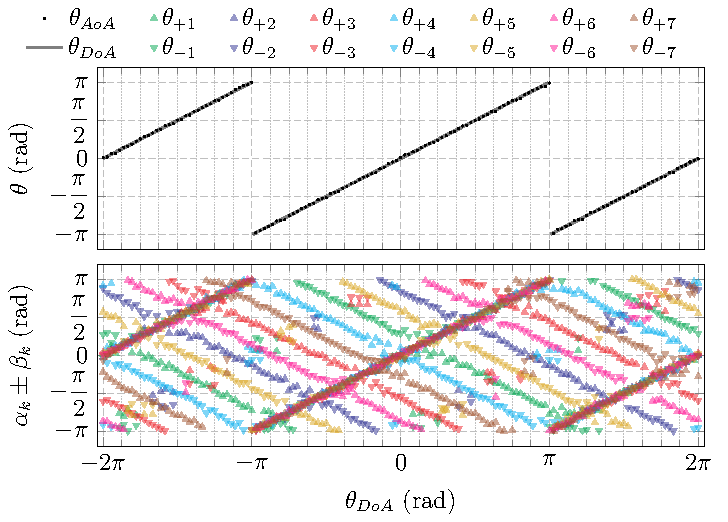
\includegraphics[height=0.785\textheight]{../pictures/simul_POLY_7_R_50_SNR_1_ATT.pdf}
			\caption*{\tiny Fonte: Autor, saída gráfica disponível em \href{https://github.com/HeckRodSav/TG/blob/main/documentation/pictures/POLY_7/simul_POLY_7_R_50_SNR_1_ATT.gif}{\underline{GitHub}}.}
		\end{figure}
	\end{frame}
